\documentclass[%
	fontsize=12pt,
	headinclude,
	paper=a4,
	numbers=noenddot,
	changebar,      % Änderungsbalken mit \begin/\end{changebar}
	listof=totoc,	% Was alles in der Table of Contents stehen soll
	bibliography=totoc,
	index=totoc,
	]{diplomarbeit}
	% noheadsepline

\areaset[20mm]{160mm}{240mm}	% Binderand, Breite und Höhe nutzbarer Bereich
\usepackage[textwidth=160mm,textheight=240mm]{geometry}

\usepackage{amssymb,amsmath}

\usepackage{color}
\usepackage{fancyvrb}

% bright ansi colors
\definecolor{darkgray}{gray}{0.25}
\definecolor{lightred}{rgb}{1.0,0.39,0.28}
\definecolor{lightgreen}{rgb}{0.48,0.99,0.0}
\definecolor{lightblue}{rgb}{0.53,0.81,0.92}
\definecolor{lightpurple}{rgb}{0.87,0.63,0.87}
\definecolor{lightcyan}{rgb}{0.5,1.0,0.83}

% commands and environments needed by pandoc snippets
% extracted from the output of `pandoc -s`
\providecommand{\tightlist}{%
  \setlength{\itemsep}{0pt}\setlength{\parskip}{0pt}}
\DefineVerbatimEnvironment{Highlighting}{Verbatim}{commandchars=\\\{\}}
% Add ',fontsize=\small' for more characters per line
\newenvironment{Shaded}{}{}
\newcommand{\KeywordTok}[1]{\textcolor[rgb]{0.00,0.44,0.13}{\textbf{{#1}}}}
\newcommand{\DataTypeTok}[1]{\textcolor[rgb]{0.56,0.13,0.00}{{#1}}}
\newcommand{\DecValTok}[1]{\textcolor[rgb]{0.25,0.63,0.44}{{#1}}}
\newcommand{\BaseNTok}[1]{\textcolor[rgb]{0.25,0.63,0.44}{{#1}}}
\newcommand{\FloatTok}[1]{\textcolor[rgb]{0.25,0.63,0.44}{{#1}}}
\newcommand{\CharTok}[1]{\textcolor[rgb]{0.25,0.44,0.63}{{#1}}}
\newcommand{\StringTok}[1]{\textcolor[rgb]{0.25,0.44,0.63}{{#1}}}
\newcommand{\CommentTok}[1]{\textcolor[rgb]{0.38,0.63,0.69}{\textit{{#1}}}}
\newcommand{\OtherTok}[1]{\textcolor[rgb]{0.00,0.44,0.13}{{#1}}}
\newcommand{\AlertTok}[1]{\textcolor[rgb]{1.00,0.00,0.00}{\textbf{{#1}}}}
\newcommand{\FunctionTok}[1]{\textcolor[rgb]{0.02,0.16,0.49}{{#1}}}
\newcommand{\RegionMarkerTok}[1]{{#1}}
\newcommand{\ErrorTok}[1]{\textcolor[rgb]{1.00,0.00,0.00}{\textbf{{#1}}}}
\newcommand{\NormalTok}[1]{{#1}}



% Additional commands for more recent versions of Pandoc
\newcommand{\ConstantTok}[1]{\textcolor[rgb]{0.53,0.00,0.00}{{#1}}}
\newcommand{\SpecialCharTok}[1]{\textcolor[rgb]{0.25,0.44,0.63}{{#1}}}
\newcommand{\VerbatimStringTok}[1]{\textcolor[rgb]{0.25,0.44,0.63}{{#1}}}
\newcommand{\SpecialStringTok}[1]{\textcolor[rgb]{0.73,0.40,0.53}{{#1}}}
\newcommand{\ImportTok}[1]{{#1}}
\newcommand{\DocumentationTok}[1]{\textcolor[rgb]{0.73,0.13,0.13}{\textit{{#1}}}}
\newcommand{\AnnotationTok}[1]{\textcolor[rgb]{0.38,0.63,0.69}{\textbf{\textit{{#1}}}}}
\newcommand{\CommentVarTok}[1]{\textcolor[rgb]{0.38,0.63,0.69}{\textbf{\textit{{#1}}}}}
\newcommand{\VariableTok}[1]{\textcolor[rgb]{0.10,0.09,0.49}{{#1}}}
\newcommand{\ControlFlowTok}[1]{\textcolor[rgb]{0.00,0.44,0.13}{\textbf{{#1}}}}
\newcommand{\OperatorTok}[1]{\textcolor[rgb]{0.40,0.40,0.40}{{#1}}}
\newcommand{\BuiltInTok}[1]{{#1}}
\newcommand{\ExtensionTok}[1]{{#1}}
\newcommand{\PreprocessorTok}[1]{\textcolor[rgb]{0.74,0.48,0.00}{{#1}}}
\newcommand{\AttributeTok}[1]{\textcolor[rgb]{0.49,0.56,0.16}{{#1}}}
\newcommand{\InformationTok}[1]{\textcolor[rgb]{0.38,0.63,0.69}{\textbf{\textit{{#1}}}}}
\newcommand{\WarningTok}[1]{\textcolor[rgb]{0.38,0.63,0.69}{\textbf{\textit{{#1}}}}}



% Define a nice break command that doesn't care if a line doesn't already
% exist.
\def\br{\hspace*{\fill} \\* }
% Math Jax compatability definitions
\def\gt{>}
\def\lt{<}
% Document parameters
% \usepackage{subcaption}
% \expandafter\def\csname ver@subfig.sty\endcsname{}

\usepackage{bibgerm}		% Für geralpha.bst. MUSS vor babel stehen
\usepackage[utf8]{inputenc}	% Latin1 input encoding (umlauts)
\usepackage[ngerman,english]{babel}
\usepackage{csquotes}       % ensure that quotes are typeset in main language

 
\usepackage[
    backend=biber,
    style=numeric-comp,
    sorting=ynt
]{biblatex}
\addbibresource{mendeley.bib}


\usepackage{parskip}		% seperate paragraphs by skip (blank line)
%\usepackage{amsfonts,amsmath,amssymb,array} % choose if needed
%\usepackage{ae,aecompl}	% Benutze 'Almost European' Zeichensatz         
%\usepackage{type1cm}	% Computer Modern type 1 fonts
\usepackage{lmodern}	% Latin Modern nehmen, da mehr Glyphen vorhanden 
\usepackage[T1]{fontenc}	% Verwende T1-Kodierung für Zeichensätze        

\usepackage{textcomp} % to make ° work


\usepackage{changebar}
\usepackage{makeidx}\makeindex

\usepackage[table,dvipsnames,svgnames,x11names,hyperref]{xcolor}
\definecolor{ColorLink}{rgb}{0,0.4549,0.8510}
\colorlet{ColorAlternatedRow}{lightgray!25}
\definecolor{DiagramRed}{HTML}{B85450}
\definecolor{DiagramGreen}{HTML}{82B366}
\definecolor{DiagramBlue}{HTML}{6C8EBF}
\definecolor{DiagramGray}{HTML}{666666}


\usepackage{graphicx}
\graphicspath{{gfx/}{gfx/boards/}{gfx/diagrams/}{gfx/figures/}{gfx/logos/}{gfx/models/}{gfx/pictures/}{gfx/results/}{gfx/screenshots/}}
\usepackage[export]{adjustbox} % https://tex.stackexchange.com/a/124372/142289
\usepackage{svg}
\usepackage{mdframed}
\usepackage{subcaption}
\usepackage{calc}         % for \svgscale

% https://tex.stackexchange.com/questions/42619/x-mark-to-match-checkmark
\usepackage{pifont}% http://ctan.org/pkg/pifont
\newcommand{\cmark}{\ding{51}}%
\newcommand{\xmark}{\ding{55}}%

\usepackage{longtable}
\usepackage{ltablex}
\usepackage{booktabs}
\usepackage{tabu}



\usepackage{pdflscape} % for 'landscape' environment


\usepackage{amsmath}


\arbeitsart{Master's Thesis}

\title{Radar Reprojection Mapping Improves Obstacle Avoidance in Mobile Robots with an Unsteered Radar Sensor}
\author{Laurenz Altenmüller}
\authorsaddr{Pommernstr. 9\\
             80809 München}
\betreuer{Michael Balszun, M.Sc.}
\ausgefuehrtam{at BSH Home Appliances Corporation\\Bosch Research and Technology Center\\Palo Alto, California, USA}
\eingereicht{September 2017}


\pdfcompresslevel=9

\makeatletter


\PassOptionsToPackage{hyphens}{url}
\usepackage[ % some option can only be set at loading time
    bookmarks=true,
    pagebackref=true,
    hyperfootnotes=false,
    pdfpagelabels=true,
]{hyperref}
\hypersetup{
    unicode=true,
	linktoc=all,
    plainpages=false,
    breaklinks=true,
    % für die DRUCK-Ausgabe
%    plainpages=false,
%    allcolors=black ]{hyperref} 
% PDF stuff    
    colorlinks=true,
    allcolors=ColorLink,
    pdfborder={0 0 0},
	pdftitle={\@title},
	pdfauthor={\@author},
	pdfsubject={Master's Thesis},
	pdfkeywords={Radar,Reprojection Mapping,Obstacle Sensor,Mobile Indoor Robots},
}
\urlstyle{same}
	
\makeatother



\begin{document}


\renewcommand{\thepage}{t\arabic{page}}
\maketitle

\begin{abstract}
    Mobile indoor robots mostly rely on lidar and vision sensors to remotely detect obstacles in their path. These sensors have trouble detecting some common real-world obstacles like transparent surfaces and chair legs. Recent affordable near-range miniature radar sensors enable new solutions.\\
    This thesis introduces a simple solution for a radar sensor being moving through a static environment without the need for beamforming or a mechanically scanning radar. The idea is put to test in experiments with an Omniradar FMCW radar mounted on a Kobuki robot platform. A comparison with lidar and RGBD sensors shows how promising the setup is for mapping unstructured static environments.
    
    ~\\
    
    Mobile Indoor-Roboter nutzen vorallem Lidar und Vision Sensoren um Hindernisse auf dem Weg aus der Entfernung zu erkennen. Diese Sensoren können einige für die echte Welt relevante Hindernisse wie transparente Flächen und Stuhlbeine jedoch nicht detektieren. Neu verfügbare Miniatur-Radarsensoren für Kurzreichweiten ermöglichen hier neue Lösungen.\\
    Diese Arbeit präsentiert eine unkomplizierte Lösung zur Kartierung statischer Umgebungen mit einem Radarsensor. Der Sensor muss bewegt, aber nicht gescannt werden und macht so Beamforming und mechanische Drehung überflüssig. Das Konzept wird in Experimenten mit einem Omniradar FMCW Radarsensor auf einer Kobuki Roboterplattform validiert. Der Vergleich mit Lidar und RGBD-Sensoren zeigt das Potential des Setups für die Erkundung unstrukturierter Umgebungen.
\end{abstract}


\pagestyle{empty}
\cleardoublepage 
\setcounter{page}{3}	% Laut VDI Richtlinien
\renewcommand{\thepage}{\roman{page}}
\begin{danksagung}
    Vielen Dank \dots
    
    München, im Monat Jahr
\end{danksagung}


\clearpage
\pagestyle{headings}
\pdfbookmark[1]{\contentsname}{toc}
\tableofcontents

\phantomsection
\begin{listofabbrevs}
\begin{tabbing}

sp	\= symbol-space---- \= \kill \+ \\

ADC \> Analog-Digital Converter \\
AESA \> Active Electronically Scanned Array \\
AMCL \> Adaptive Monte Carlo Localization \\
API \> Application Programming Interface \\
BSH \> Bosch Siemens Hausgeräte \\
CFAR \> Constant False Alarm Rate \\
CW \> Continuous wave \\
DAC \> Digital-Analog-Converter \\
DOA \> Direction Of Arrival \\
DK \> Development Kit \\
EM \> Electromagnetic \\
FCC \> Federal Communcations Commision \\
FFT \> Fast Fourier Transform \\
FMCW \> Frequency modulated continuous wave \\
FOV \> Field Of View \\
FPGA \> Field Programmable Gate Array \\
FWHM \> Full Width at Half Maximum \\
GNSS \> Global Navigation Satellite System \\
IC \> Integrated Circuit \\
IEEE \> Institute of Electrical and Electronics Engineers \\
IF \> Intermediate Frequency \\
IMU \> Intertial Measurement Unit \\
IR \> InfraRed \\
ISM \> Industrial, Scientific, Medical \\
LIDAR \> LIght Detection and Ranging \\
LO \> Local Oscillator \\
MCU \> Microcontroller unit \\
MEX \> Matlab EXecutable \\
MIMO \> Multiple In, Multiple Out \\
NDA \> Non-Disclosure Agreement \\
PCB \> Printed Circuit Board \\
PDF \> Probability Density Function \\
PLL \> Phase-Locked Loop \\
RAII \> Ressource Allocation Is Initialization \\
RCS \> Institute for Real-time Computer Systems \\*
   	\> Radar cross section \\
RDK \> Radar Development Kit \\
REP \> ROS Enhancement Proposal \\
RF \> Radio Frequency \\
RADAR \> RAdio Detection And Ranging \\
RGB \> Red/Green/Blue \\
RGBD \> Red/Green/Blue/Depth \\
RMS \> Root mean square \\
ROS \> Robot Operating System \\
RX \> Receive \\
SAR \> Synthetic Aperture Radar \\
SAS \> Synthetic Aperture Sonar \\
SCP \> Secure CoPy \\
SLAM \> Simultaneous Localization And Mapping \\
SNR \> Signal to Noise Ratio \\
SONAR \> SOund Navigation And Ranging \\
SPI \> Serial Peripheral Interface \\
TOF \> Time of Flight \\
TX \> Transmit \\
UWB \> Ultra Wide Band \\
VCO \> Voltage Controlled Oscillator \\
VSLAM \> Visual SLAM \\

\end{tabbing}
\end{listofabbrevs}

\phantomsection
\begin{listofsymbols}
\begin{tabularx}{\textwidth}{%
  >{\setlength{\hsize}{.15\hsize}\raggedright\arraybackslash}X%
  >{\setlength{\hsize}{.75\hsize}}X%
  >{\setlength{\hsize}{.10\hsize}\raggedright\arraybackslash}X%
}

$A_r$ & Effective antenna aperture \\
$c$ & Speed of light & $m/s$ \\
$d$ & Antenna separation & $m$ \\
$dR$ & Range resolution & $m$ \\
$f_a$ & Angle compensation factor \\
$f_r$ & Range compensation factor \\
$G_r$ & Receive antenna gain \\
$G_t$ & Transmit antenna gain \\
$n_{chirp}$ & Number of consecutive FMCW chirps \\
$P_r$ & Received target power \\
$P_t$ & Transmission power \\
$R$ & Target range & $m$ \\
$S_i$ & Complex antenna signal \\
$t_{chirp}$ & Duration of FMCW chirp & $s$ \\
$t_{msg}$ & Time between two ROS radar messages & $s$ \\
$v_R$ & Radar or robot movement speed & $m/s$ \\
$v_D$ & Relative Doppler speed & $m/m$ \\
$\Delta\Phi$ & Phase difference \\
$\lambda$ & Wavelength & $m$ \\
$\sigma$ & Radar cross section & $m^2$ \\
$\tau$ & Time of flight / Time delay & $s$ \\

\end{tabularx}
\end{listofsymbols}


% start with page 1
\newpage{\pagestyle{plain}\cleardoublepage}
\rmfamily
\renewcommand{\thepage}{\arabic{page}}
\setcounter{page}{1}

% content
\include{chapters/ch_input}

\chapter{Theoretical Background}\label{theoretical-background}

A variety of sensors enable robots to sense their environment. Most
robots monitor information like temperature or track odometry from
intertial measurement units (IMU) and wheel encoders. This section
focuses on how a robot can avoid or detect collisions.

\section{Traditional Obstacle
Sensors}\label{traditional-obstacle-sensors}

The fallback option of obstacle sensing is almost always a bumper
sensor. If the robot runs into an obstacle in its path, a bumper switch
will be pressed and the robot's navigation system knows that it can not
traverse further in this particular direction. The concept can be
extended to measure sudden acceleration that indicates a collision or
even monitor motor current to find that the robot is stuck against an
obstacle, but the idea is the same: With this kind of sensor, the robot
can only detect that it already had a collision. The detection can be
shifted to slightly earlier point in time with systems like whisker-like
antennae or capacitive sensors\cite{Muhlbacher-Karrer2015}. A special
case is negative obstacle (e.g.~cliff) detection. Here, usually Infrared
(IR) range sensors are employed on the underside of the robot.

Intelligent navigation and path planning however can only be achieved
with ranging sensors. Classic range sensors are IR, ultrasound (US), or
laser based. They measure the distance to the closest target in one
direction. Because obstacles can appear in any direction, these sensors
need to be scanned. Scanning means that the bearing of active sensing
direction is changed over time to achieve range scans that are
multiplexed over a field of view (FOV). Usually this is done
mechanically, with a sensor turret spinning on a servo motor. The best
known example of this is the classic lidar sensor, which spins a laser
range finder around.

Vision sensors are scannerless. Next to regular cameras as monocular
vision sensors there are stereo-camera setups to record depth
information. Structured light sensors such as the first-generation
Microsoft Kinect sensor record depth disparity from triangulation, via
correlation between a known and perceived projected light pattern.
Time-of-flight (TOF) cameras like the second-generation Microsoft Kinect
illuminate the scene with amplitude-modulated near-IR light and
calculate depth from the phase shift between the transmitted and
received signal\cite{Sarbolandi2015}.

There is also a scannerless version of lidar. Full-field lidar, also
known as flash lidar \cite{Payne2008} uses TOF measurements of
omnidirectional light pulses to capture a 2D scene.

To map out the environment and localize itself, the robot will usually
employ a version of a simultaneous localization and mapping (slam)
algorithm\cite{Cadena2016}.

\section{Radar}\label{radar}

Radar sensing is based on the transmission and reflection of
electromagnetic signals. A transmitting antenna radiates EM energy, some
of which is scattered off reflective objects, called targets, and
intercepted by a receiving antenna. This signal is amplified and checked
for time delay, frequency shift, phase shift and amplitude attenuation
with respect to the transmitted signal. This allows to capture certain
target properties like range, radial velocity, size, shape and, among
others, even surface smoothness and orientation. \cite{Skolnik2008}

The return signal's echo power is described for the interference-free
case in vacuum by the radar equation, \[
P_r = 
\frac{P_t G_t}{4\pi R^2}
\cdot
\frac{\sigma}{4\pi R^2}
\cdot
A_r
\] where \(P_r\) received target echo power \(P_t\) transmission power
\(G_t\) transmit antenna gain \(R\) range of target (distance)
\(\sigma\) radar cross section (RCS) of target \(A_r\) effective area of
receiving antenna. Of the three factors in the equation, the first
factor represents the power density at the radar-illuminated target's
distance. The second factor represents how much of the radar energy is
scattered back by the target. The third factor finally denotes how much
of the echo power is collected by the receiving antenna.
\cite{Skolnik2008} Conventional radar only becomes useful with directive
antennas. The antenna gain \(G_t\) is defined as the ratio of increased
power in a particular direction compared with that from an isotropic
antenna \cite{Adams2012}. Antenna theory shows \cite{Balanis2015} the
relation of receive antenna gain \(G_r\) with radiation wavelength
\(\lambda\): \[G_r = \frac{4\pi A_r}{\lambda^2}\] With constant antenna
loss factor \(L>1\), substituting equation \#REF into equation \#REF
yields the classical radar equation \[
P_r =
\frac{P_t G_t G_r \lambda^2 \sigma}{(4\pi)^3R^4L}
\propto \frac{\sigma}{R^4}
\] In practice, the actual received power is lower than predicted by
this equation due to many factors, including interference and
atmospheric conditions. \(\sigma\) is also not constant but varies with
viewing angle and material properties of the target. \cite{Adams2012}

\subsection{Doppler effect}\label{doppler-effect}

Many radar systems measure radial velocity with the Doppler frequency
shift. Austrian physicist Christian Doppler described the kinematic
effect in 1842. It describes the change of wavelength caused by the
motion. A common example is the change of pitch that can be heard when a
race car or ambulance passes the observer. The Doppler frequency shift
\(f_D\) is \[
f_D = 2 \frac{v_r}{\lambda} = 2 \frac{v \cos ( \theta )}{\lambda}
\] where \(v_r\) is the radial velocity component of the target, which
travels at a speed \(v\) at angle \(\theta\) between the target's
direction and the radar beam with wavelength \(\lambda\)
\cite{Skolnik2008}. The factor \(2\) is caused by the Doppler shift
being applied twice; once for the incident wave, and once for the
reflected wave. In effect this means that a radar sending out an EM wave
with a frequency of exactly \(60GHz\) towards a target moving at a
relative speed of \(v_r = 1\frac{cm}{s}\) towards the radar will receive
back an echo with a frequency of \(60000000004 Hz\) because of the
frequency shift of \(f_D = 4 Hz\).

\subsection{Types of Radar}\label{types-of-radar}

\subsubsection{Continuous Wave (CW) radar}\label{continuous-wave-cw-radar}

CW radar was the first radar system. It uses a continuous transmission
at a fixed frequency. Thanks to antenna directionality it can be used to
find a target's azimuth in radio direction finding. A target's velocity
information can be extracted from the frequency shift due to the Doppler
effect.

\subsubsection{Pulse radar}\label{pulse-radar}

Pulse radars send series of short bursts. The time delay \(\tau\)
between transmission and reception of a pulse, called time of flight
(TOF), gives a target's range \(R\), so that \[ R = \frac{c\tau}{2} \]
The range resolution \(\Delta R\) is given by
\[\Delta R = \frac{c\tau_m}{2}\] with \(\tau_m\) the pulse high time. To
achieve high range resolution pulses must be very short, which requires
very high peak transmission power to still produce a detectable echo
signal. Pulse compression radars send a longer pulse with an internal
modulation, which combines the higher transmission energy of longer
pulses with the resolution of short pulses. Velocity is again known from
frequency shift.

\begin{figure}[htp]
    \centering
    \label{fig:radar_pulse}
    \def\svgwidth{\linewidth}
    \input{gfx/diagrams/radar_pulsed.pdf_tex}
    \caption{Pulse radars measure the time between stransmission and reception of a short EM burst. Adapted from \cite{Adams2012} p.~52}
\end{figure}


\subsection{Frequency-modulated continuous wave (FMCW)
radar}\label{frequency-modulated-continuous-wave-fmcw-radar}

FMCW radars use a frequency modulation to measure range and speed at the
same time. The transmitted modulation is compared to the modulation in
the received signal to detect signal delay and frequency shift.
Applications in robotics use this kind of radar the most, for reasons of
lower transmission power and high-range resolution \cite{Adams2012}.

An FMCW radar's modulation is called a frequency sweep or chirp and is
usually triangular with a linearily increasing and decreasing frequency.
Most sensor use a voltage controlled oscillator (VCO) to generate the
modulation waveform. VCOs do not have a linear transfer function, so in
order to obtain a linear sweep, the input to the VCO must be
pre-distorted with the inverse of the VCO's nonlinear transfer function.
Instead of a VCO, direct digital synthesizers together with phase-locked
loops (PLL) can be used. They generate better (more linear) sweeps at
the price of increased design complexity and cost \cite{Ernst2016}.

\begin{figure}[htp]
    \centering
    \label{fig:fmcw_blocks}
    \def\svgwidth{\linewidth}
    \input{gfx/diagrams/fmcw_blocks.pdf_tex}
    \caption{Simplified FMCW architecture. Adapted from \cite{VanZeijl2014}}
\end{figure}

After the VCO's signal is amplified and transmitted, it reflects at
visible targets and is received as echo in the same frequency band.

\begin{figure}[htp]
    \centering
    \label{fig:fmcw_triangular}
    \def\svgwidth{\linewidth}
    \input{gfx/diagrams/fmcw_triangular.pdf_tex}
    \caption{FMCW radars detect targets in the beat frequency, which is a frequency mix of the transmitted and received modulation. Adapted from \cite{Adams2012} p.~57}
\end{figure}

In the top subplot, figure \ref{fig:fmcw_triangular} shows the transmitted frequency sweep
from \(f_0\) to \(f_0 + \Delta f\) over a sweep length of \(T_d\) of a
triangular modulation. The middle plot also shows the received signal as
caused by a single stationary ideal reflector. Time of flight causes a
delay \(\tau\) in the received signal. To understand where the beat
signal comes from, we focus on the rising part of the triangle
modulation, the upsweep. Using the superheterodyne principle the
received signal \(v_{Rx}\) and a portion of the transmitted signal
\(v_{Tx}\) (called the local oscillator (LO)), are frequency mixed in an
analog multiplier to get the intermediate frequency (IF) \(v_{Mixer}\).
The IF contains a target's beat frequency, which is proportional to the
target's range. With the transmitted signal \(v_{Tx}\) and the received
signal \(v_{Rx}\) as a function of time \(t\), \[
\begin{aligned}
v_{Tx}(t) &= A_{Tx} \cos\bigl(\omega_{Tx}(t)~t\bigr)\\
v_{Rx}(t) &= A_{Rx} \cos\bigl(\omega_{Tx}(t-\tau)~t\bigr)\\
\end{aligned}
\] where \(\omega_{Tx}\) is the angular frequency of the transmitted
signal, \[
\begin{aligned}
\omega_{Tx}(t) &= \underbrace{\omega_c}_\text{Carrier frequency} + \underbrace{\pi \frac{\Delta f}{T_d} t}_\text{Upsweep modulation}
\end{aligned}
\] the signal behind the frequency mixer \(v_{Mixer}\) can be calculated
as \[
\begin{aligned}
v_{Mixer}(t) &= v_{Tx}(t) ~ v_{Rx}(t) \\
&= A_{Tx}A_{Rx}~\cos(t\omega_{Tx}(t))t~\cos(\omega_{Tx}(t-\tau)t)
\end{aligned}
\] With the trigonometric identity
\[ \cos A \cdot \cos B = \frac{ \cos(A+B)~+~\cos(A-B) }{2} \]
\(v_{Mixer}\) can be written as \[
v_{Mixer}(t-\tau) = \frac{A_{Tx} A_{Rx}}{2}(B_1 + B_2)
\] where \[
\begin{aligned}
B_1 &= \cos\bigl[ 2\omega_{Tx}(t-\tau) t - \omega_{Tx}(\tau)\tau \bigr]\\
    &= \cos\left[ 2\left(\omega_c + \pi\frac{\Delta f}{T_d}(t-\tau)\right)t - \left(\omega_c - \pi\frac{\Delta f}{T_d}\tau\right)\tau \right]\\
B_2 &= \cos\left[ 2\left(\pi\frac{\Delta f}{T_d}t\right)\tau - \omega_{Tx}(\tau)\tau \right]\\
    &= \cos\left[ 2\pi\left(\frac{\Delta f}{T_d}\tau\right)t - \left(\omega_c + \pi\frac{\Delta f}{T_d}\tau\right)\tau \right]
\end{aligned}
\] Note that \(B_1\) consists of high angular frequencies around the
carrier frequency, from \(f_0 = \frac{\omega_c}{2\pi}\) to
\(f_0 + \Delta f\). \(B_2\) is a lower frequency (theoretically up to
\(2\pi\Delta f\) at \(\tau = T_d\), but much lower in practice, as echos
from targets this far away have very low intensity \(A_{Rx}\) and can't
be detected) signal containing the beat frequency. The output of the
low-pass filter intrinsic in the mixer stage will thus only consist of
the beat frequency (plus noise of similar frequencies): \[
v_{beat}(t,\tau) = \frac{A{Tx}A_{Rx}}{2} \cos \left[ 2\pi\left(\frac{\Delta f}{T_d}\tau\right)t - \left(\omega_c + \pi\frac{\Delta f}{T_d}\tau \right) \tau \right]
\] The term \(\frac{\Delta f}{T_d}\tau\) in \(v_{beat}(t,\tau)\) is
known as the beat frequency \(f_b\). For stationary targets, the
range-specific frequency \(f_R = f_b\). Knowing that the delay time
\(\tau\) depends on the speed of light \(c\) and the range \(R\), the
relationship between a target's \(f_R\) and range \(R\) can be given as
\[
f_R = \frac{2R}{c} \frac{\Delta f}{T_d} \iff R=\frac{c T_d}{2\Delta f}f_R
\] This also gives the range resolution \(dR\), \[
dR = \frac{c}{2 \Delta f}
\]

\begin{figure}[htp]
    \centering
    \label{fig:fmcw_doppler}
    \def\svgwidth{\linewidth}
    \input{gfx/diagrams/fmcw_doppler.pdf_tex}
    \caption{Target motion introduces a Doppler shift in the received signal, which changes the beat frequency during up- and down-sweep. Adapted from \cite{Adams2012} p.~57}
\end{figure}

A moving target however will introduce a Doppler shift \(f_D\) in the
received signal \(v_{Rx}\), which will shift the target's beat frequency
\(f_b\) away from its range-specific frequency \(f_R\). The direction of
the frequency shift depends on the modulation: An up-sweep will have a
corresponding \[f_{b,up} = f_R - f_D\] while the down-sweep has
\[f_{b,down} = f_R + f_D\] The range-specific frequency and Doppler
frequency can be extracted from the two beat frequencies by averaging
them: \[
\begin{aligned}
f_R &= \frac{f_{b,down} + f_{b,up}}{2} \\
f_D &= \frac{f_{b,down} - f_{b,up}}{2}
\end{aligned}
\]

The benefit of the triangular sweep becomes clear here: with a sawtooth
waveform, only \(f_b,up\) can be determined. A stationary target and a
moving target a range and Doppler speed corresponding to the same
resulting frequencies would not be distinguishable.

Of course, more than one target can be visible at a time. If multiple
echos are received, as in figure \ref{fig:radar_fmcw_multitarget}, the intermediate frequency will
contain multiple frequencies. The beat signal will have more than one
dominant frequency in its spectrum, with each one corresponding to a
different target.

\begin{figure}[htp]
    \centering
    \label{fig:fmcw_multitarget}
    \def\svgwidth{\linewidth}
    \input{gfx/diagrams/fmcw_multitarget.pdf_tex}
    \caption{Each target contributes a frequency corresponding to its range in the beat spectrum.}
\end{figure}

Figure \ref{fig:fmcw_multitarget} shows a real-world example of how the beat signal \(f_b\)
(top subplot) and its frequency spectrum (bottom subplot) look like. At
\(t=T_d=32ms\), a jump in the beat frequency is caused by the modulation
change from upsweep to downsweep. In the frequency spectrum, three
stationary targets are visible at ca. \(3kHz\), \(6kHz\), and \(9kHz\).
In this example, \(T_d=32ms\) and \(\Delta f=7GHz\), so the targets were
at ranges of \(0.5m\), \(1m\), and \(1.5m\). Note that the in-phase part
\(S_I\) and quadrature part \(S_Q\) of the analytic signal are measured
in separate channels to retain phase information. The Fourier transform
in bottom subplot however shows the magnitude \(\|S\|\) of the analytic
signal\footnote{A good explanation is available at [ping.se's I/Q Data for Dummies](http://whiteboard.ping.se/SDR/IQ)}
\(S = S_I + j~S_Q\) with the imaginary unit \(j\).

\begin{figure}[htp]
    \centering
    \label{fig:fig_raw_beat}
    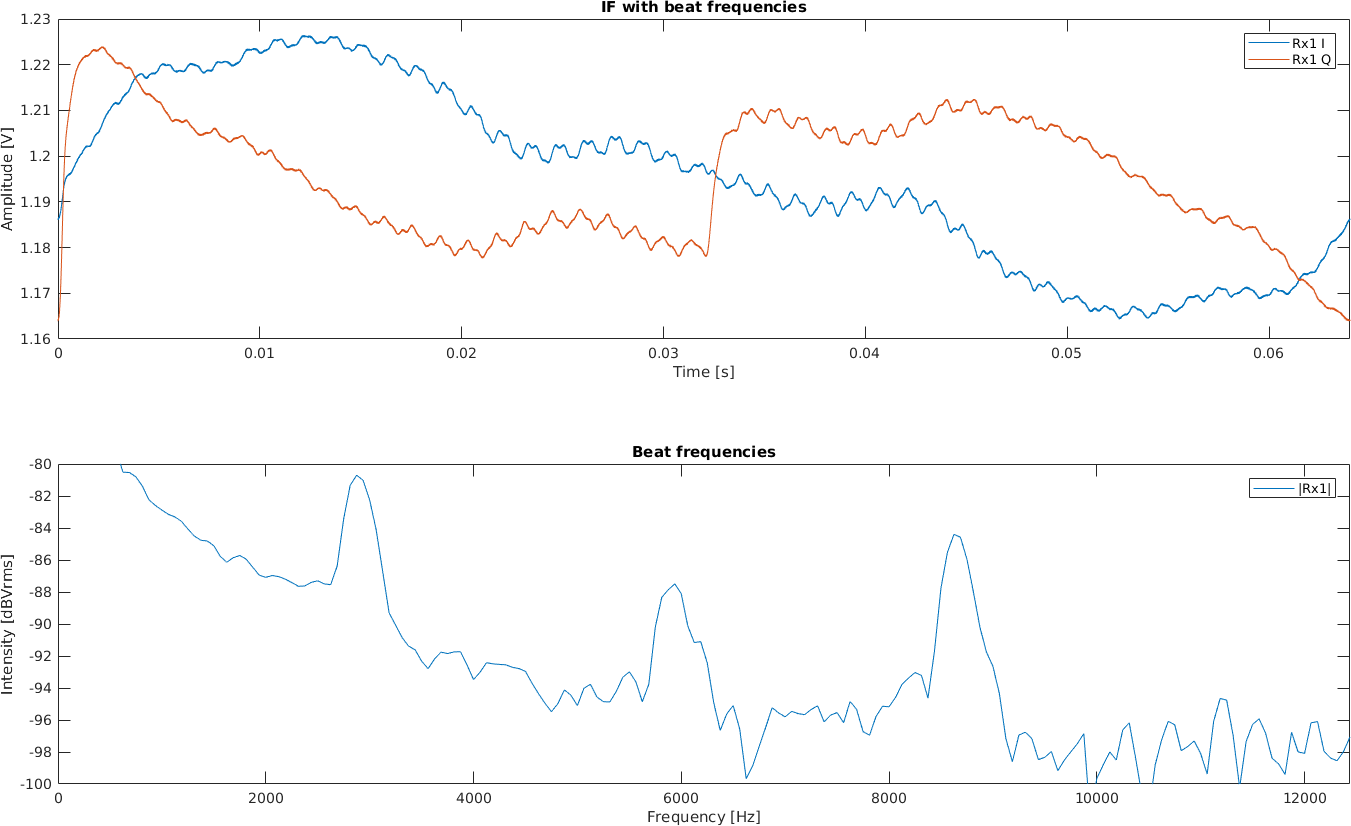
\includegraphics[max height=10cm,max width=10cm]{figures/fig_raw_beat.png}
    \caption{Beat signal and spectrum / range profile in a real-world measurement.}
\end{figure}

\subsection{Direction of Arrival}\label{direction-of-arrival}

A radar sensor with two or more receiving antennas which are separated
by not more than half a wavelength can measure the Direction of arrival
(DOA) of one or multiple targets. Because the echo from a target has to
travel a slightly longer distance to antennas further away, a phase
difference between the different antenna signals is measurable.

In the case of a pair of receiving antennas, the direction of arrival
\(\theta\) can be estimated \cite{VanZeijl2014} as

\[\theta = sin^{-1}\left({\frac{\lambda~\Delta\Phi}{2\pi ~d}}\right)\]

with wavelength \(\lambda\), antenna separation \(d\) and phase
difference \(\Delta\Phi\). \(\Delta\Phi\) is the angle difference
\(\angle S_1 - \angle S_2\) of the complex analytic antenna signals
\(S = S_I + j~S_Q\).

\begin{figure}[htp]
    \centering
    \label{fig:doa}
    \def\svgwidth{\linewidth}
    \input{gfx/diagrams/doa.pdf_tex}
    \caption{Direction of Arrival \(\theta\) can be estimated from phase difference \(\Delta\Phi\)}
\end{figure}

TODO
\cite{Hacker2010} \cite{Cho2017}

\subsection{Frequencies}\label{frequencies}

Even though radar applications exist for many frequencies, only a few of
them are OK to use for radiolocation and in home robots. The
``Industrial, Scientific, Medical'' (ISM) bands allows the unlicensed
use of some frequencies for radiolocation, including center frequencies
of \(24.125 GHz\), \(61.25 GHz\), \(122.5 GHz\) and \(245 GHz\).
Applications must however accept harmful interference \cite{FCC2017}.

The \(77 GHz\) band is ``restricted to vehicle-mounted field disturbance
sensors used as vehicle radar systems.'' (FCC Part 15 §15.253(c)) - ETSI
defines it as ``Automatic Cruise Control `long-range radar' operating at
\(77 GHz\). This enables a vehicle to maintain a cruising distance from
a vehicle in front.'' (EN 301 091). The German Bundesnetzagentur also
declares it ``Kraftfahrzeug-Kurzstreckenradar'' (Vfg 66 / 2014).

A \(24 GHz\) center frequency is a safe bet. There are many radar
systems available and it being an ISM band makes licensing much easier.
The drawback is the very limited maximum bandwidth of \(250MHz\) in this
band.

Some newer radars use the \(60 GHz\) ISM band. It allows a rather wide
bandwidth of up to \(9GHz\) in some regions (see figure \ref{fig:wigig} ).
According to equation \#REF, this gives a very good range resolution in
the order of few \(cm\). At these high frequencies, RF energy
attenuation in material increases noticably \cite{FerrisJr.1998}. The
effect is that \(60GHz\) waves are limited to short ranges of a few
\(m\) and don't usually penetrate walls.

\begin{figure}[htp]
    \centering
    \label{fig:attenuation}
    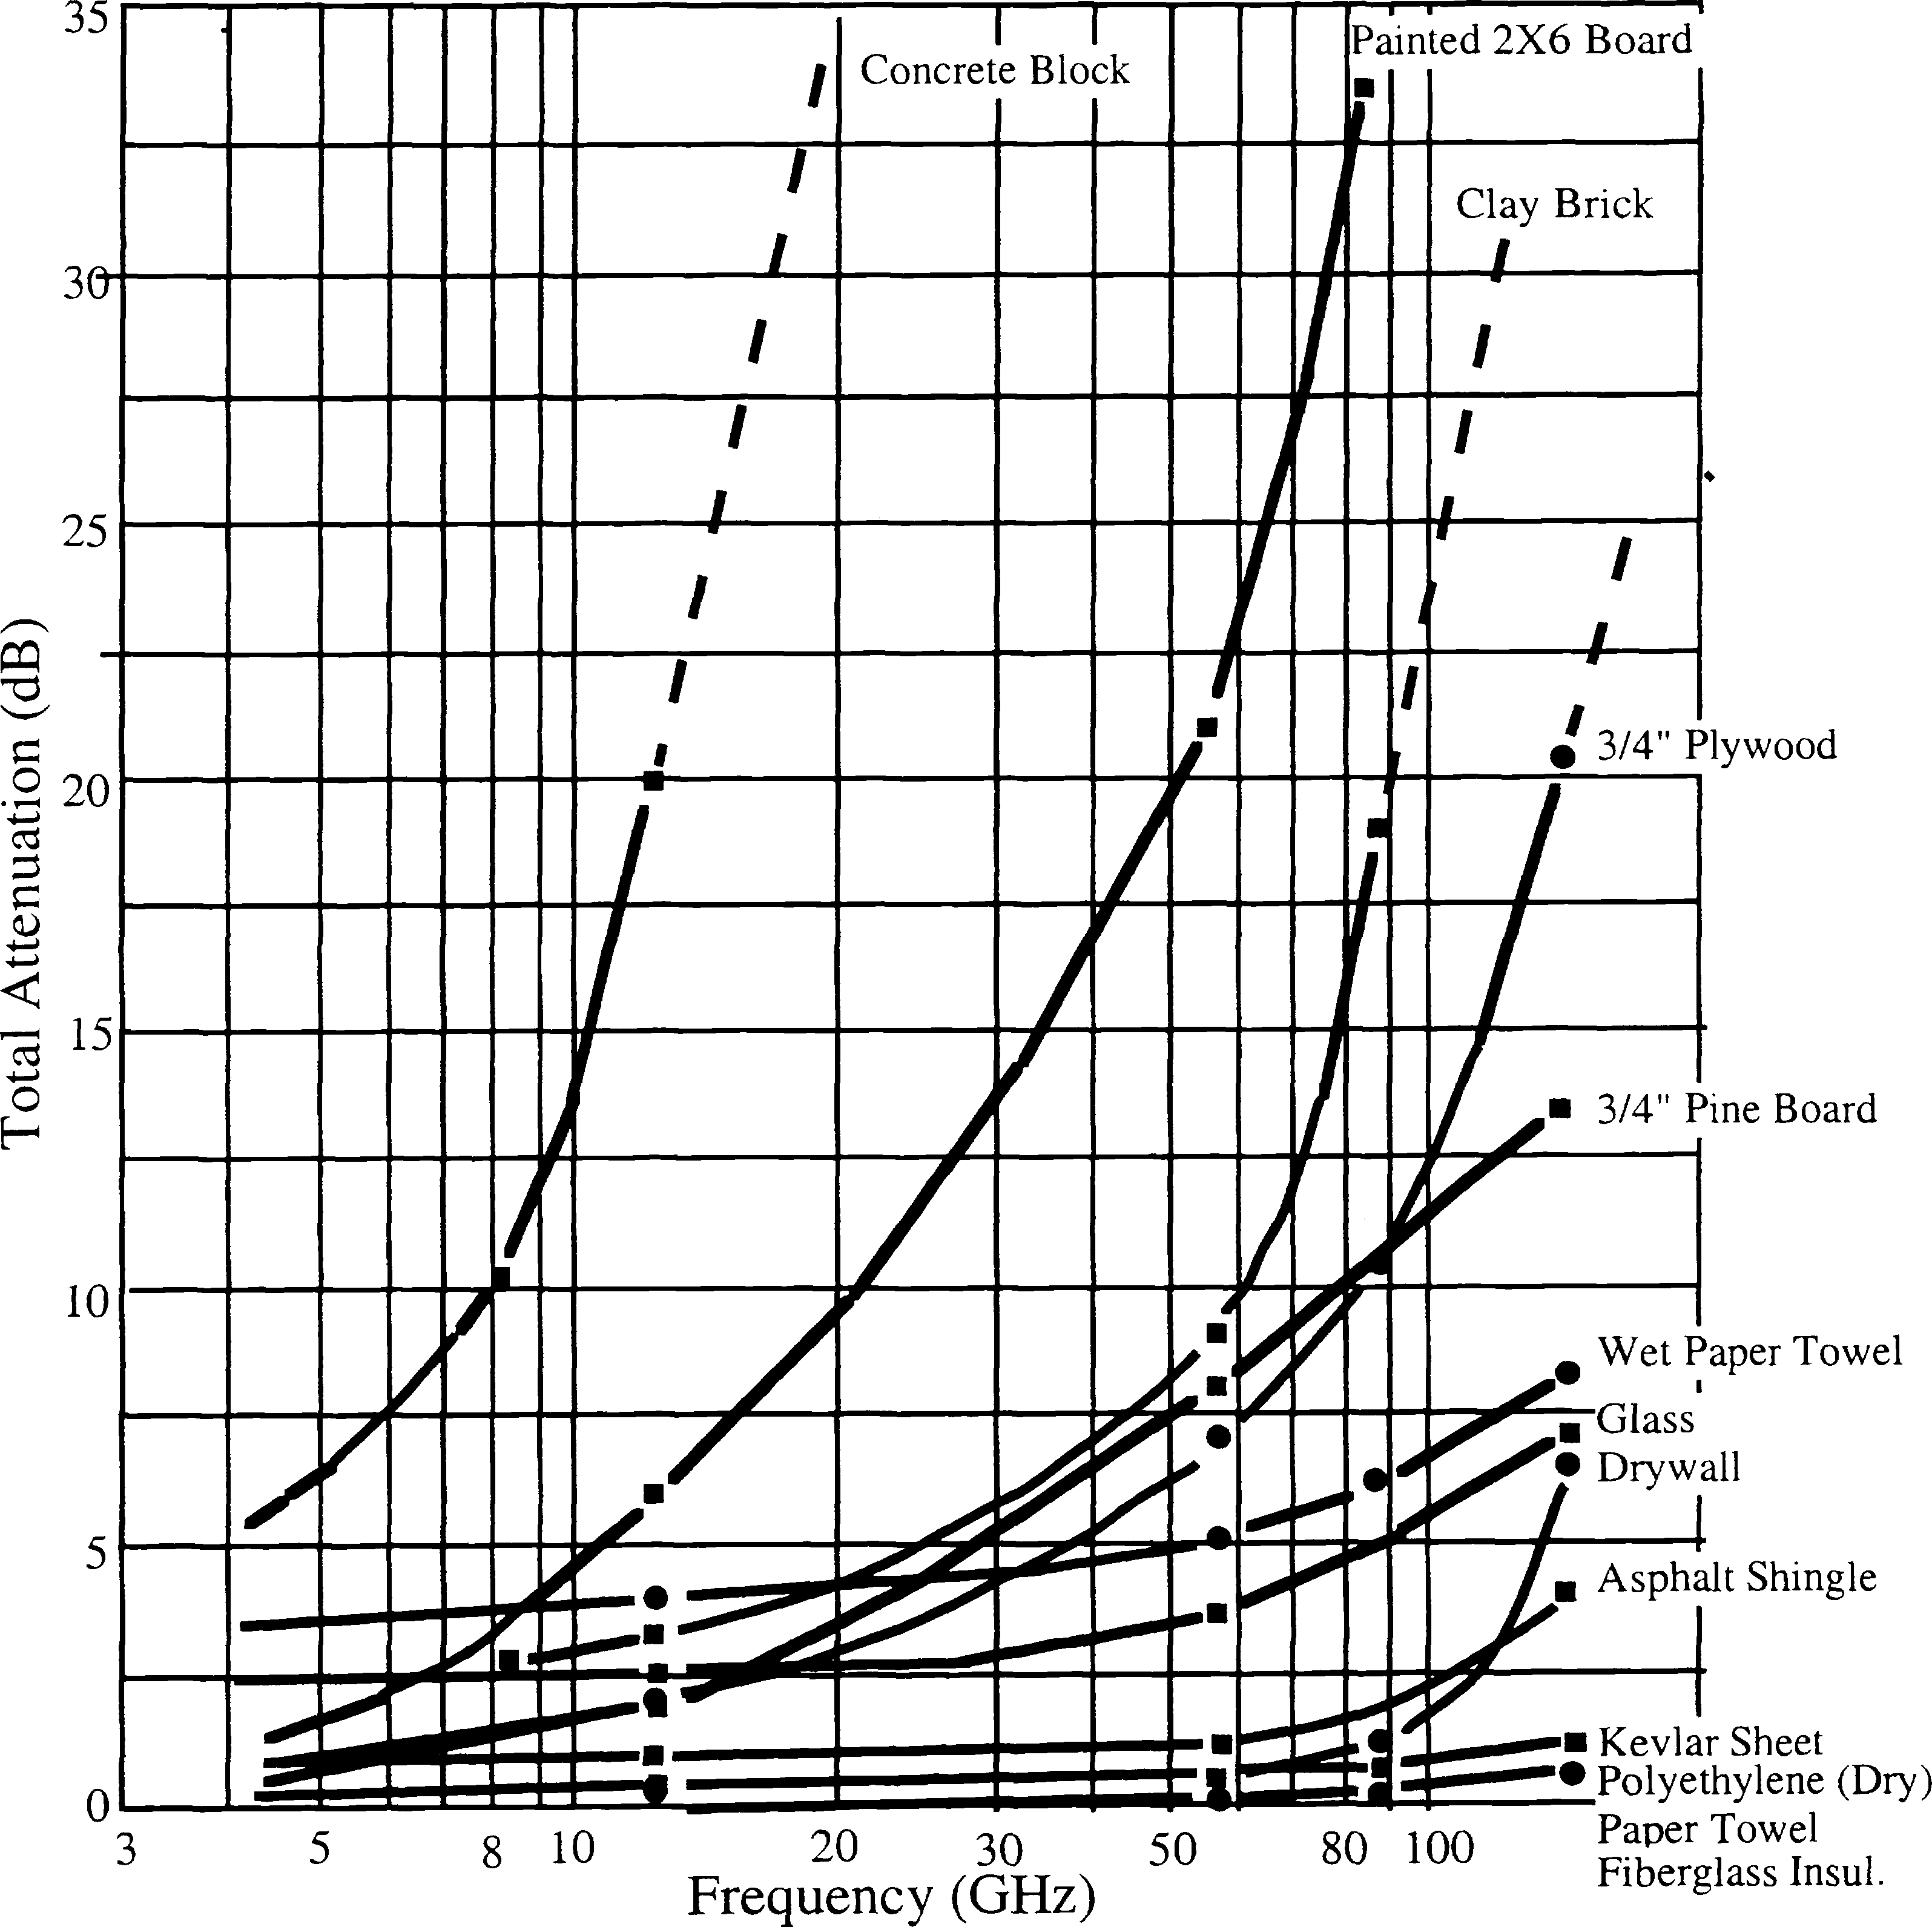
\includegraphics[max height=10cm,max width=10cm]{figures/rf_attenuation}
    \caption{Totl attenuation of RF energy when transmitted through various materials as a function of frequency. Source: \cite{FerrisJr.1998}}
\end{figure}

Atmospheric attenuation also limits long-range applications. In short
range (a few \(m\)) it should however not present a problem.

\begin{figure}[htp]
    \centering
    \label{fig:attenuation_air}
    
\includegraphics[max height=10cm,max width=10cm]{figures/ITU_0676-05}
    \caption{Specific RF attenuation due to atmospheric gases. Source: \cite{ITU1997}}
\end{figure}

The downside is that there are some other technologies using the same
frequency bands, most notably 802.11ad a.k.a.
WiGig\cite{AgilentTechnologies2013}. The WiGig frequency allocations in
figure \ref{fig:wigig} show in which regions the \(60GHz\) band is available (also
for radar).

\begin{figure}[htp]
    \centering
    \label{fig:wigig}
    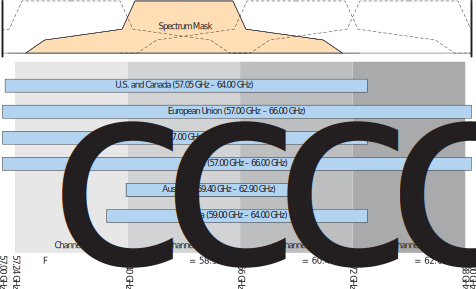
\includegraphics[max height=10cm,max width=10cm]{diagrams/spectrum}
    \caption{WiGig Channel Plan and Frequency Allocations by Region. Source: \cite{AgilentTechnologies2013}}
\end{figure}

\section{Overview of Radar
Research}\label{overview-of-radar-research}

Radar is used and researched since the 1940s. While it was historically
only used to detect aircraft and ships, it is an active research domain
in many fields today. Identification and localization of vessels is of
course still an important application in both civil and military
sectors. There is a great amount of research going into synthetic
aperture radar, in terrestrial imaging, but also general and concealed
imaging. Another area of research is radar antenna technology and
quasi-optics, which aims to find design improvements and more adapted
antennas for the manifold applications. Radar is used in human presence
detection and monitoring, including heartbeat detection. A new and very
promising discipline is radar-based gesture recognition, which enables
innovative human machine interaction applications. Indoor communication
and localization with radar beacons is another interesting and upcoming
technology. The radar-related research area that is most relevant for
mobile robots is radar-based slam.

\section{Existing radar-based solutions for map
building}\label{existing-radar-based-solutions-for-map-building}

\subsection{SAR}\label{sar}

In 1950 Doppler frequency analysis was found to improve image resolution
of side-looking radar, which led to the development of the synthetic
aperture radar (SAR) technique. SAR uses azimuth (along-track) motion to
synthesize an aperture that is longer than the physical size of the
radar antenna \cite{Wang2008}. The three major configurations are
stripmap SAR, scan SAR, and spotlight SAR. Current SAR systems can
operate in either mode by dividing their planar antenna into
sub-apertures, whose phase and amplitude are controlled by the
individual few hundred transmit/receive modules \cite{Moreira2013}.

\begin{figure}[htp]
    \centering
    \label{fig:sarmodes}
    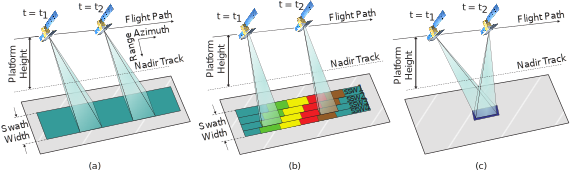
\includegraphics[max height=10cm,max width=10cm]{diagrams/sar}
    \caption{Illustration of different SAR operation modes which are used to increase the swath width (ScanSAR) or improve azimuth resolution (Spotlight) compared to Stripmap mode.
    (a) Stripmap. (b) ScanSAR. (c) Spotlight. Source: \cite{Moreira2013}}
\end{figure}

Radar echo data is sampled in both fast-time and slow-time, with
fast-time meaning the range scan dimension (fast, because the EM waves
travel at very high speed, \(c\)) and slow time denoting the azimuth or
along-track dimension (slow, because movement velocity will be
\(\ll c\)). This raw data does not give any useful information and needs
to be signal-processed first. Because SAR systems typically use
pulse-compressed radars, each range line needs to be convoluted with the
complex conjugate of the transmitted chirp's spectrum to obtain the
range-compressed
data\footnote{For the FMCW system used in the later parts of this thesis this is not necessary - the FMCW beat frequency spectrum is equivalent to the range-compressed data}.
In a second step, azimuth compression takes place by convolving the
signal in slow-time with the complex conjugate of the expected
azimuth-response from a target.

\begin{figure}[htp]
    \centering
    \label{fig:sarsteps}
    \includegraphics[max height=10cm,max width=10cm]{diagrams/sar2}
    \caption{Summary of SAR processing steps where the range compressed data result from a convolution of the raw data with the range reference function. In a second step the azimuth compression is performed through a convolution with the azimuth reference function, which changes from near to far range. Source: \cite{Moreira2013}}
\end{figure}

An elemental scatterer at range \(R(t)\) will return an echo \(s_a(t)\)
over time \(t\): \[
s_a(t) = P_r \sqrt{\sigma\vphantom{1}} \exp(j\varphi_s)\exp(j \underbrace{\frac{-4\pi}{\lambda}R(t)}_\text{az. phase var. $\omega_D$})
\] where \(P_r\) is the echo power of the received target, accounting
for dependencies like transmit power and path loss, \(\sigma\) is the
target's RCS, imaginary unit \(j\), \(\varphi_s\) the scattering phase,
and \(\frac{4\pi}{\lambda}R(t)\) the azimuth phase variation due to
changing distance \cite{Cumming2004}. The target's range \(R(t)\) is
described by the range at closest approach \(R_0\) and the radar's
(constant) movement speed \(v_R\): \[
R(t) = \sqrt{R_0^2+\left(v_Rt\right)^2} \approx R_0 + \frac{(v_Rt)^2}{2R_0} ~\text{for}~ \frac{v_Rt}{R_0} \ll 1
\] Substituting \#REF into the azimuth phase in \#REF and derivating
with respect to time yields the azimuth frequency \(f_D\) \[
\begin{aligned}
f_D &= \underbrace{\frac{1}{2\pi}}_{\omega_D = 2\pi f_D} \frac{\partial}{\partial t} \frac{-4\pi}{\lambda}  \underbrace{\left( R_0 + \frac{(v_Rt)^2}{2R_0}  \right)}_{R(t)} \\
&= -\frac{2v_R^2}{\lambda R_0}t
\end{aligned}
\] The azimuth frequency varies linearly with time \(t\) and is
inversely proportional to the closest approach (slant range) \(R_0\),
hence the azimuth reference function depends on geometry and is adapted
to range. Because of the frequency-shifting effect it is analogous to
and also called the Doppler frequency.

The most challenging aspect of SAR is the correction of range cell
migration induced defocusing. Range cell migration is visible in figure
\ref{fig:sarsteps}'s curvature of range compressed data. It occurs when a point
target's echo energy is distributed over several range cells, causing
azimuth defocusing. This effect is range-variant, as the curvature
depends on \(R_0\). Hence a non-stationary two-dimensional reference
function is necessary. There are several approaches in tackling this,
including the omega-k / wavenumber processor, range-Doppler, and chirp
scaling algorithms \cite{Moreira2013}.

\subsection{Scanning radar}\label{scanning-radar}

TODO

Small ground robots

\begin{itemize}
\item
  Martin Adams
\item
  Henrik Forsten
\item
  Gregory Charvat
\item
  Bat type radar
\end{itemize}

\subsection{Radar slam}\label{radar-slam}

TODO

Radar Slam

\begin{itemize}
\item
  Martin Adams
\item
  K2Pi
\end{itemize}


\chapter{Novel Approach: Reprojection
Mapping}\label{novel-approach-reprojection-mapping}

\section{Idea}\label{idea}

With the Reprojection method, a radar echo's source can be determined
without scanning the radar sensor. The distance to a target is already
available in the radar data, so only the direction is needed to update a
map. Under certain circumstances, this direction can also be extracted
from the sensor's data.

The prerequisite to the method is that the sensor has to move with a
known speed \(v_R\) through an otherwise static environment. Caused by
the radar's motion, the distance to all visible targets changes, which
causes a Doppler speed \(v_D\) for every target point.

\subsection{Geometry for the side-facing
case}\label{geometry-for-the-side-facing-case}

If the radar is moving directly towards a target, the target's Doppler
speed \(v_D\) will be equal to radar speed \(v_R\) (target \(A\) in
figure \ref{fig:geometry_side}). If the radar passes the target on the side, so that the
distance to the target stops decreasing and begins to grow, \(v_D = 0\)
(target \(C\) in figure). If a target has an absolute Doppler speed
\(\|v_D\|\) between \(0\) and \(v_R\) (target \(B\) in figure), it is seen
from the radar under an angle \(\alpha\), such that
\[v_D = v_R cos(\alpha)\]

\begin{figure}[htp]
    \centering
    \label{fig:geometry_side}
    \def\svgwidth{\linewidth}
    \input{gfx/diagrams/geometry_side.pdf_tex}
    \caption{Reprojection geometry for the side-facing case}
\end{figure}

Positive values for \(\alpha\) indicate targets on the left side of the
robot, while negative values for \(\alpha\) indicate right hand side
targets. The caveat is that from \(v_D\) only the absolute value of
angle \(\alpha\) is known. This is OK if the radar is mounted
side-facing, such that only targets on one side of the motion path are
visible. Like this, the angle ambiguity is resolved, because only one
side is visible.

\subsection{Geometry for the General
case}\label{geometry-for-the-general-case}

In the general case such as with a forward facing radar, or with radar
antennas with angle sensitivities that allow a field of view of over
\(180^\circ\), the angle ambiguity must be resolved differently.

\begin{figure}[htp]
    \centering
    \label{fig:geometry_general}
    \def\svgwidth{\linewidth}
    \input{gfx/diagrams/geometry_forward.pdf_tex}
    \caption{Reprojection geometry for the general 2D case}
\end{figure}

One solution to resolving the angle ambiguity is to use direction of
arrival (DOA) information from a multistatic radar. If the radar is
facing straight forward, a target's DOA will be lower or higher,
depending on the antenna configuration and the side the target is being
passed on. If the radar is not facing straight but still has parts of
both sides of the motion paths visible in it's FOV the DOA gradient
should be used instead of its value: If a target's DOA is gradually
shifting towards left (i.e.~lower or higher, depending on the system),
it will pass the radar on the left side. If it is gradually shifting
towards right, it will pass on the right side.

\subsection{Reprojection Method}\label{reprojection-method}

TODO

When a target's range and angle are known, it can be mapped in relation
to the radar's position.

This allows intelligent path planning and obstacle avoidance for mobile
robots.



\subsection{Peak Gradient algorithm}\label{peak-gradient-algorithm}

TODO

One pillar of the Reprojection Method is the Doppler speed of static
targets. If the Doppler speed is not precisely measured, the
reprojection angle \(\alpha\) is imprecise or noisy, which leads to
smeared-out targets or even false positive detections on the map.

With FMCW radar, a target's range and Doppler speed can be
simultaneously registered.

\subsection{Limitations}\label{limitations}


TODO

\chapter{Implementation}\label{implementation}

The validity and performance of reprojection mapping is put to test with a proof of concept implementation in Matlab for a system based on an Omniradar RIC60-A mounted on a Kobuki robot platform.

\section{Implementation Platform}\label{implementation-platform}

\subsection{Kobuki}\label{kobuki}

The reprojection method requires that the radar is moved through the scene with a known position and velocity. The Kobuki robot platform (shown in \cref{fig:kobuki}) was developed by Yujin Robot\footnote{\url{http://kobuki.yujinrobot.com/}}, a Korean robotics and toy company. As base for the second Turtlebot, the reference design for the Robot Operating System (ROS), it not only provides a fairly good odometry system, but also allows to move the radar in a controlled way. Its shape and performance are very comparable to a real-world vacuum robot (it is actually based off Yujin's iClebo vacuum robot series), which makes the application relatively realistic.

\begin{figure}[htbp]
    \centering
    \begin{subfigure}{0.45\textwidth}
        \includegraphics[max width=\linewidth]{models/kobuki}
        \caption{Yujin's iClebo Kobuki robot platform. Source: \cite{DesignK2013}}
        \label{fig:kobuki}
    \end{subfigure}
    \hfill
    \begin{subfigure}{0.45\textwidth}
        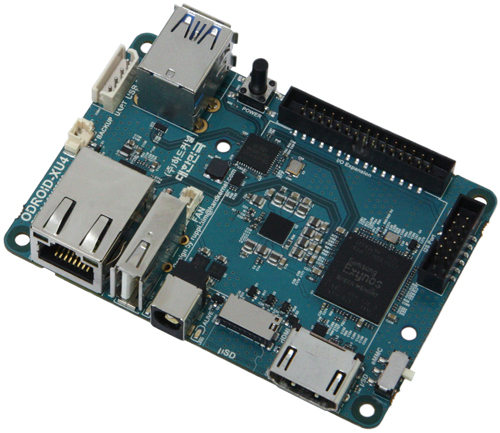
\includegraphics[max width=\linewidth]{pictures/odroid}
        \caption{Hardkernel Odroid XU4. Source: \url{https://wikimedia.org/wiki/File:Hardkernel_Odroid_XU4_Board.jpg}}
        \label{fig:odroid}
    \end{subfigure}
\end{figure}

\subsection{ROS integration}\label{ros-integration}

The Robot Operating System (ROS)\footnote{\url{http://www.ros.org/}} is widely used in robotics research. It provides a framework of robotic hardware drivers, software libraries with state-of-the-art algorithms, and powerful developer tools for building robot applications. The Kobuki ROS package\footnote{\url{http://wiki.ros.org/kobuki}} is widely used and tested. With \texttt{rosbag}s, the ROS system also provides a convenient way to record data for later playback and analysis.

\subsection{Odroid}\label{odroid}

In the Kobuki platform, only an embeddded microcontroller is integrated to drive the robot's hardware. ROS however needs an OS to run on and a computing platform with at least some performance. In this implementation, Hardkernel's Odroid XU4\footnote{\url{http://www.hardkernel.com/main/products/prdt_info.php?g_code=G143452239825}} (see \cref{fig:odroid}) single-board computer provides plenty of power with its Samsung Exynos Cortex-A15/Cortex-A7 2GHz Octa core CPUs paired with 2GB ram. It runs Ubuntu Linux 14.04 with ROS Indigo Igloo.

\subsection{Radar sensor}\label{radar-sensor}

One of the most important aspects of the implementation is the choice of radar sensor.

\subsubsection{Devkit list}\label{devkit-list}

There are quite a few short-range UWB FMCW radar modules available. They are all small enough to be integrated in a product of a size Important features are high bandwidth to achieve high range resolution, good update rate, and easy configuration and integration of both hardware and software. Of course the sensor must also be available for sampling or purchase. The following table compares some promising solutions, roughly sorted by bandwidth. $f_C$ and $\Delta f$ denote the center frequency and bandwidth of the product, respectively. Note that the development kit (DK) price is usually much higher than the price of the radar chip sold for integration in products.



\newlength{\colwidthA} \setlength{\colwidthA}{0.15\textwidth}
\newlength{\colwidthB} \setlength{\colwidthB}{0.2\textwidth}
\newlength{\colwidthC} \setlength{\colwidthC}{0.1\textwidth}
\newlength{\colwidthE} \setlength{\colwidthE}{0.10\textwidth}
\newlength{\colwidthF} \setlength{\colwidthF}{0.05\textwidth}
\newlength{\colwidthG} \setlength{\colwidthG}{0.15\textwidth}
\newlength{\maximheight} \setlength{\maximheight}{2cm}

{
\rowcolors{1}{ColorAlternatedRow}{}
\setlength\extrarowheight{4pt}
    
\begin{tabularx}{\linewidth}{%
  >{\setlength{\hsize}{.20\hsize}\raggedright\arraybackslash}X%
  >{\setlength{\hsize}{.25\hsize}}X%
  >{\setlength{\hsize}{.15\hsize}\raggedright\arraybackslash}X%
  >{\setlength{\hsize}{.15\hsize}\raggedright\arraybackslash}X%
  >{\setlength{\hsize}{.10\hsize}\raggedright\arraybackslash}X%
  >{\setlength{\hsize}{.20\hsize}\centering\arraybackslash}X%
}%
%\caption{Comparison of UWB radar development kits}\label{tab:devkits}

\hiderowcolors
\toprule
    Product &
    Note &
    $f_C$, $\Delta f$ &
    Antennas &
    DK Price &
    Picture \\
    \midrule
\endhead

\midrule
\multicolumn{6}{r}{Continued on next page} \\
\endfoot

\bottomrule
\endlastfoot
\showrowcolors

Omniradar RIC60A\footnote{\url{https://www.omniradar.com/products/}} &
High bandwidth. Presentation at SoC 2015\cite{Brouwer2015} &
60~GHz, 7~GHz &
On-chip, 1~Tx,~2~Rx &
\$4000 &
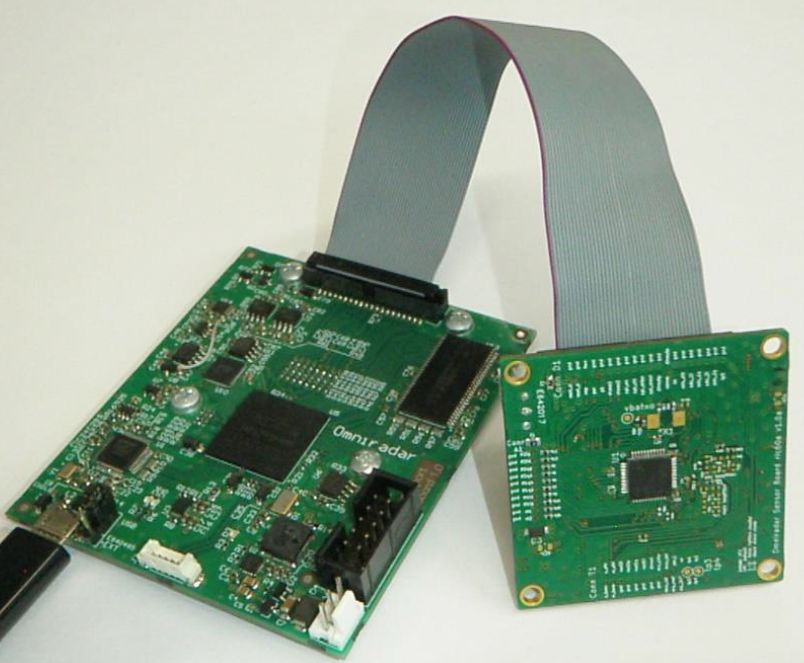
\includegraphics[max width=\hsize,max height=\maximheight,valign=t]{boards/img_omniradar.jpg}
\par\vspace{\extrarowheight}
\tabularnewline

Google / Infineon Soli\footnote{\url{https://www.infineon.com/cms/en/product/promopages/soli/}} &
Expected 2018. Sub-millimeter accuracy, running at over 10,000 frames per second \cite{Lien2016} &
60~GHz, 7~GHz &
In\nobreakdash-package, 2~Tx,~4~Rx &
? &
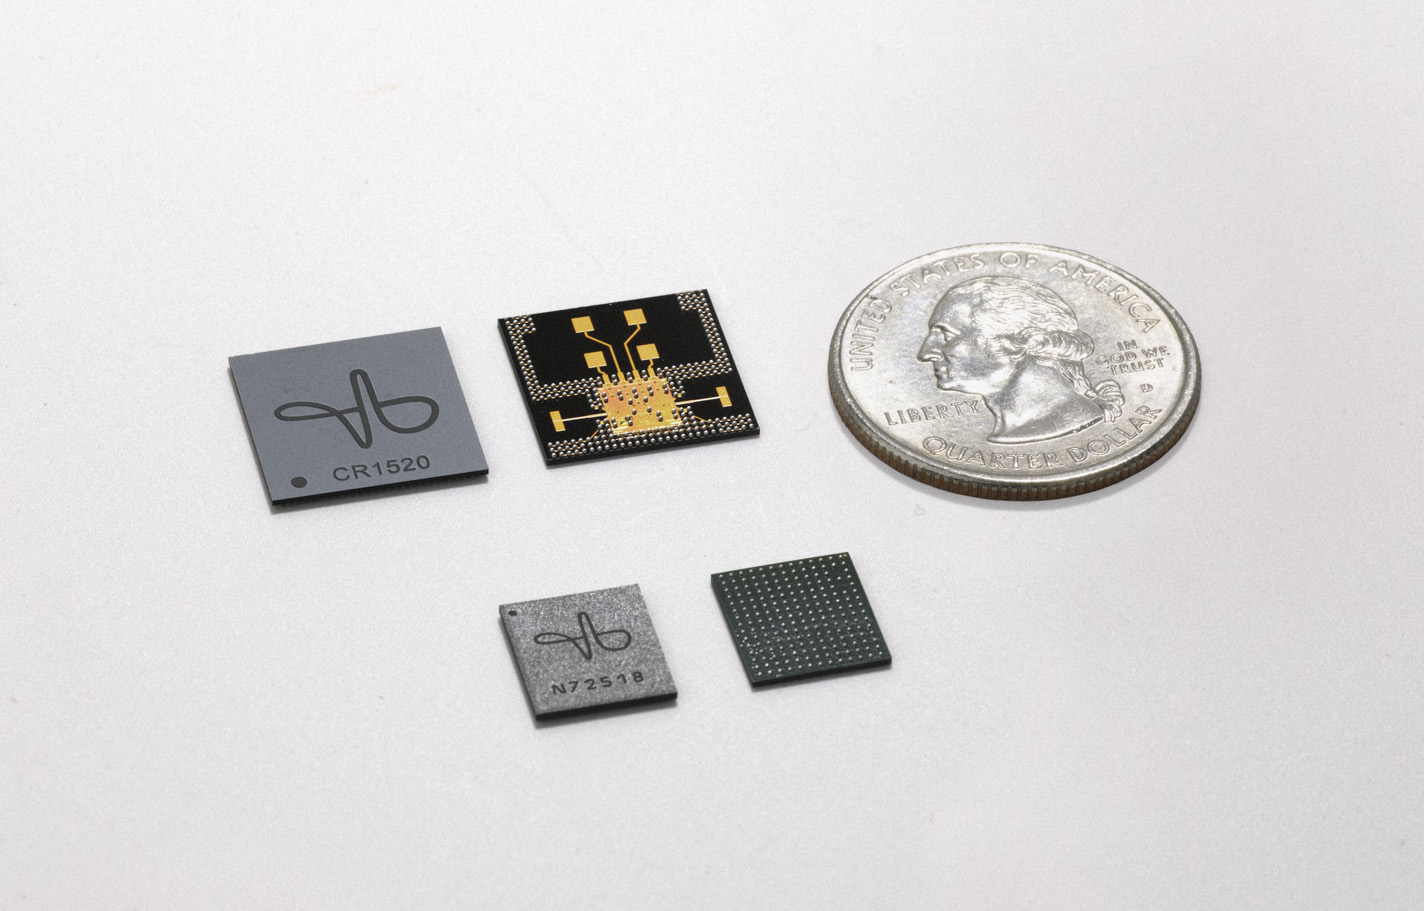
\includegraphics[max width=\hsize,max height=\maximheight,valign=t]{boards/img_soli.png}
\par\vspace{\extrarowheight}
\tabularnewline

Walabot Pro\footnote{\url{https://walabot.com/store/us/products/walabot-developer-pack.html}}&
3D configuration. Slow update rate&
6.8~GHz, 7~GHz &
On\nobreakdash-board, 9~Tx,~9~Rx&
\$599&
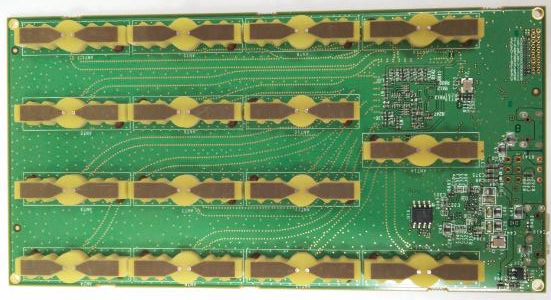
\includegraphics[max width=\hsize,max height=\maximheight,valign=t]{boards/img_walabot_1.png}
\par\vspace{\extrarowheight}
\tabularnewline

Bosch Prototype&
Prototype for In-wall pipe detection&
5.15~GHz, 6.7~GHz &
External, 2~Tx/Rx&
- &
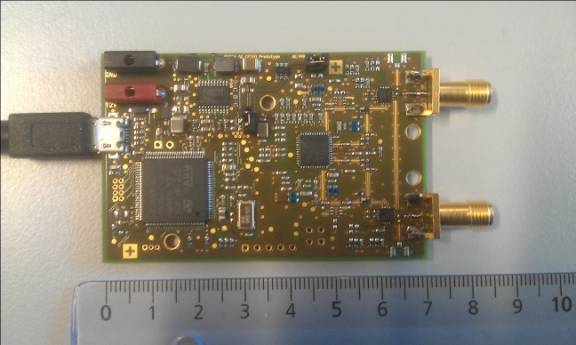
\includegraphics[max width=\hsize,max height=\maximheight,valign=t]{boards/img_bosch.jpg}
\par\vspace{\extrarowheight}
\tabularnewline

Silicon Radar SiRad Simple\footnote{\url{http://www.siliconradar.de/evalkits_e.html}}&
Has WiFi&
122~GHz, 6.4~GHz &
On-chip, 1~Tx,~1~Rx&
?&
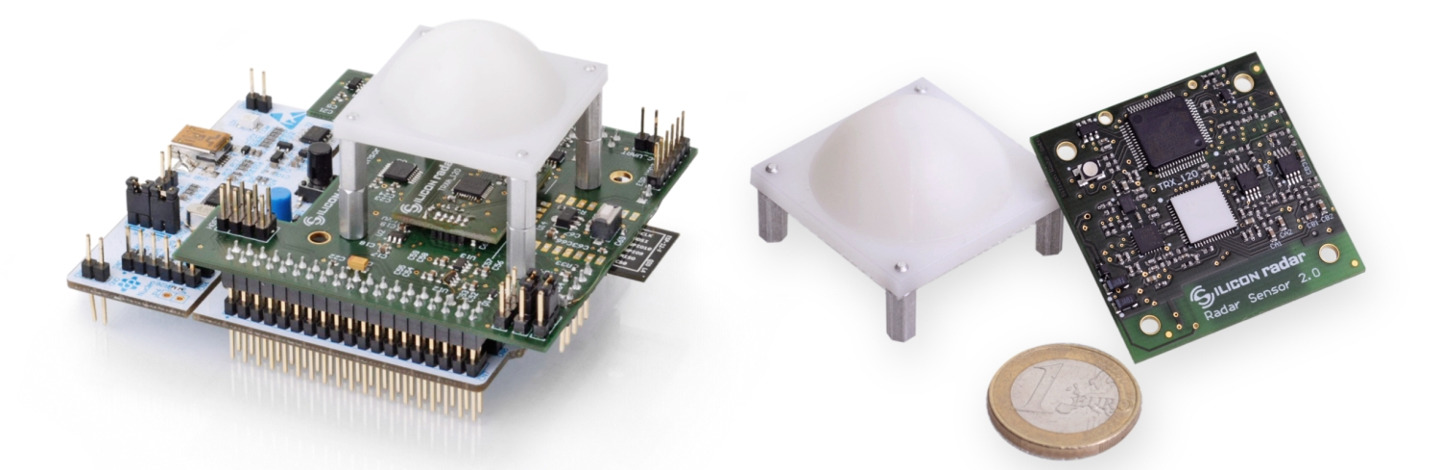
\includegraphics[max width=\hsize,max height=\maximheight,valign=t]{boards/img_silicon_radar.jpg}
\par\vspace{\extrarowheight}
\tabularnewline

Anokiwave AWMF-0117\footnote{\url{http://www.anokiwave.com/products/awmf-0117/index.html}}&
&
12.5~GHz, 4.5~GHz &
On-chip, 1~Tx/Rx&
?&
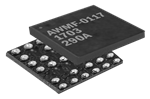
\includegraphics[max width=\hsize,max height=\maximheight,valign=t]{boards/img_anokiwave.png}
\par\vspace{\extrarowheight}
\tabularnewline

NXP Cocoon Radar\footnote{\url{Reuter2016}}&
Relatively small board. Presentation at FTF 2016\cite{Reuter2016}&
77~GHz, 4~GHz &
On\nobreakdash-board, 3~Tx,~4~Rx&
?&
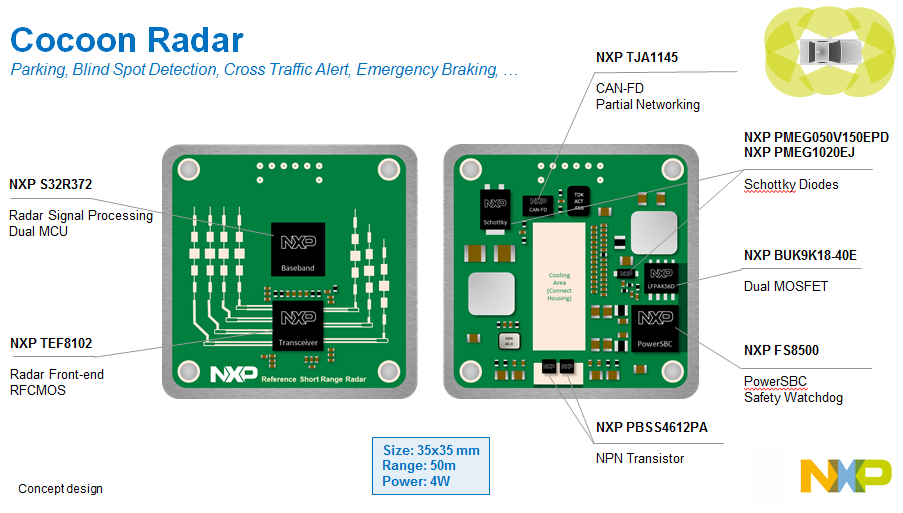
\includegraphics[max width=\hsize,max height=\maximheight,valign=t]{boards/img_cocoon.png}
\par\vspace{\extrarowheight}
\tabularnewline

TimeDomain P440\footnote{\url{http://www.timedomain.com/products/pulson-440/}}&
Can operate as multistatic radar or UWB communication node&
4~GHz, 1.7~GHz &
External, 2~Tx/Rx&
\$5000&
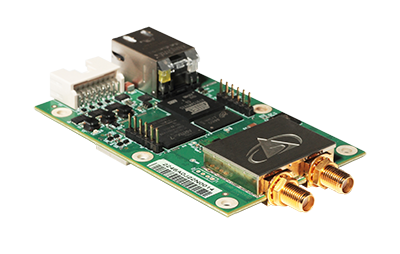
\includegraphics[max width=\hsize,max height=\maximheight,valign=t]{boards/img_p440.png}
\par\vspace{\extrarowheight}
\tabularnewline

Novelda Xethru X4M03\footnote{\url{https://www.xethru.com/xethru-development-platform.html}}&
&
8~GHz, 1.5~GHz &
On\nobreakdash-board, 1~Tx/Rx&
\$399&
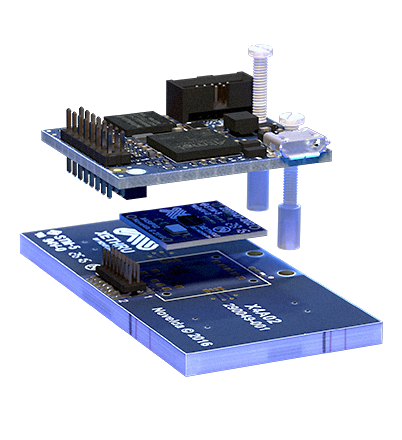
\includegraphics[max width=\hsize,max height=\maximheight,valign=t]{boards/img_xethru.png}
\par\vspace{\extrarowheight}
\tabularnewline

RFbeam MR2001\_RD\footnote{\url{https://www.rfbeam.ch/files/products/26/downloads/ProductBrief_MR2001_RD.pdf}}&
&
77~GHz, 1~GHz &
On\nobreakdash-board, 4~Tx,~6~Rx&
?&
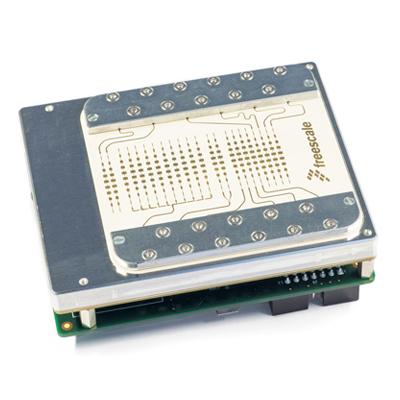
\includegraphics[max width=\hsize,max height=\maximheight,valign=t]{boards/img_rfbeam.jpg}
\par\vspace{\extrarowheight}
\tabularnewline

Inras 77Ghz Radarbook\footnote{\url{http://www.inras.at/en/products/radarbook.html}}&
Configurable FPGA processing chain&
77~GHz, 1~GHz &
On\nobreakdash-board, 4~Tx,~8~Rx&
\$7300&
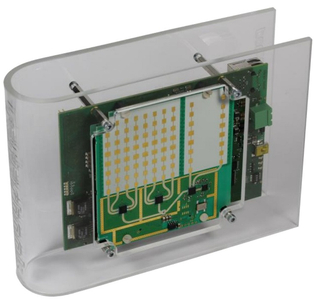
\includegraphics[max width=\hsize,max height=\maximheight,valign=t]{boards/img_radarbook.jpg}
\par\vspace{\extrarowheight}
\tabularnewline

Acconeer A1\footnote{\url{ http://www.acconeer.com/}}&
Sub-mm accuracy&
60~GHz, ? &
On-chip, ?&
?&
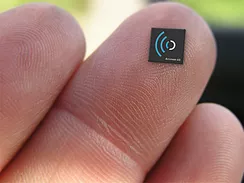
\includegraphics[max width=\hsize,max height=\maximheight,valign=t]{boards/img_acconeer.png}
\par\vspace{\extrarowheight}
\tabularnewline

Inras 24Ghz Radarbook\footnote{\url{dkradarbook}}&
&
24~GHz, 250~MHz &
On\nobreakdash-board, 4~Tx,~4~Rx&
\$7300&
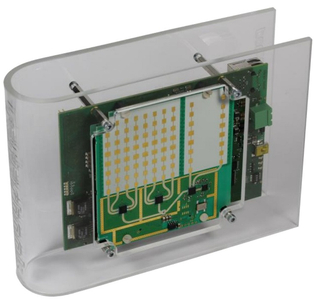
\includegraphics[max width=\hsize,max height=\maximheight,valign=t]{boards/img_radarbook.jpg}
\par\vspace{\extrarowheight}
\tabularnewline

Infineon BGT24-RFB2412-EVAL\footnote{\url{https://www.infineon.com/dgdl/?fileId=5546d46259d9a4bf0159f9f1fa503f1d}}&
&
24~GHz, 250~MHz &
On\nobreakdash-board, 1~Tx,~2~Rx&
\$1333&
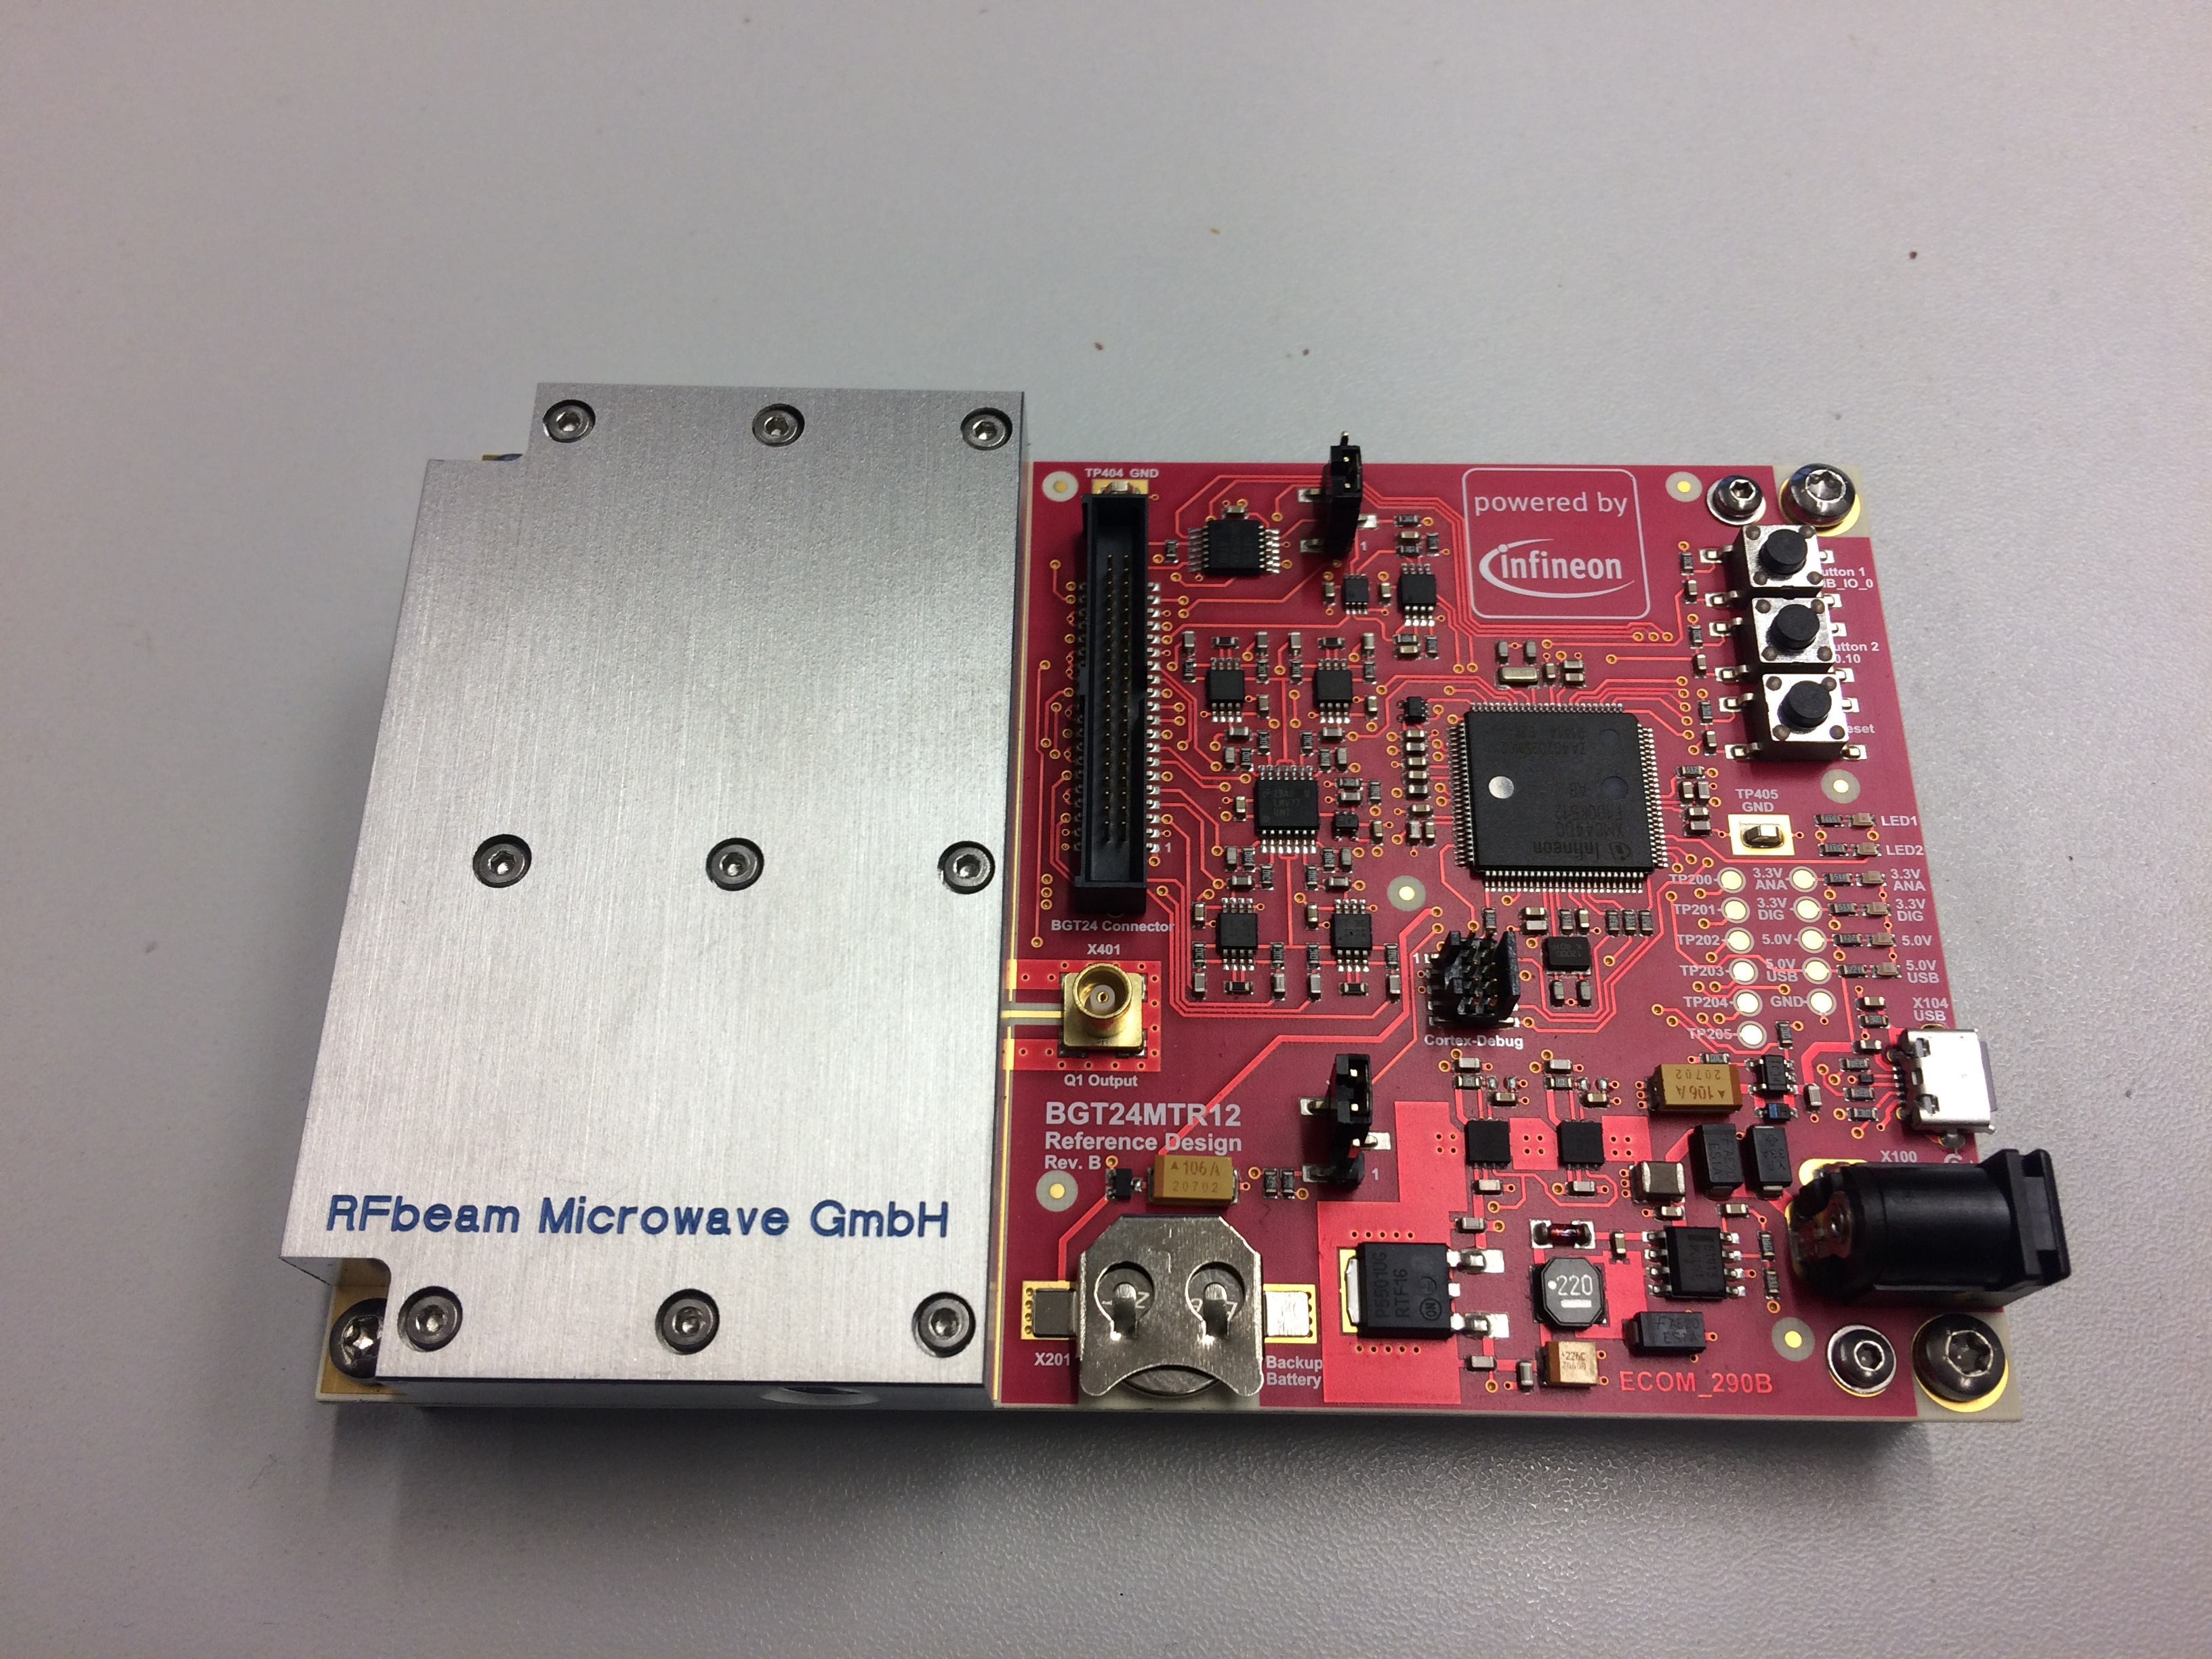
\includegraphics[max width=\hsize,max height=\maximheight,valign=t]{boards/img_bgt24.JPG}
\par\vspace{\extrarowheight}
\tabularnewline

IMST DK-sR-1200e\footnote{\url{http://webshop.imst.de/dk-sr-1200e-development-platform-for-24-ghz-fmcw-radar-application.html}}&
&
24~GHz, 250~MHz &
On\nobreakdash-board, 1~Tx,~2~Rx&
\$3333&
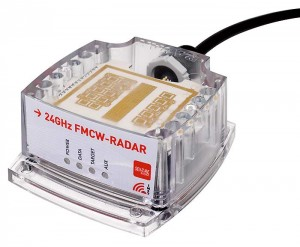
\includegraphics[max width=\hsize,max height=\maximheight,valign=t]{boards/img_IMST.jpg}
\par\vspace{\extrarowheight}
\tabularnewline

InnoSenT IVS-565\footnote{\url{http://www.innosent.de/fileadmin/media/dokumente/DATASHEETS_2016/Datenblatt_IVS-565.pdf}}&
&
24~GHz, 250~MHz &
On\nobreakdash-board, 1~Tx,~2~Rx&
?&
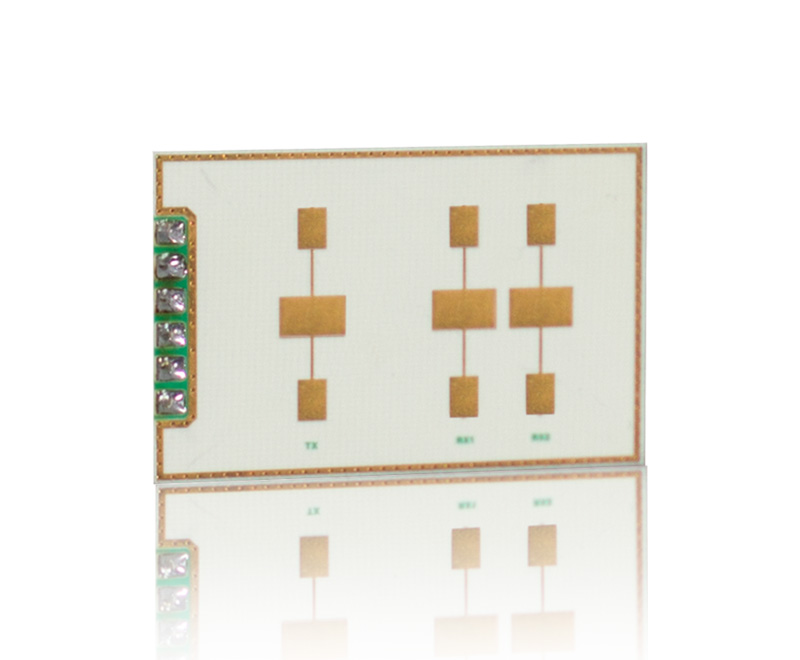
\includegraphics[max width=\hsize,max height=\maximheight,valign=t]{boards/img_innosent.jpg}
\par\vspace{\extrarowheight}
\tabularnewline

ST EVB-STradA431\footnote{\url{http://www.st.com/content/st_com/en/products/evaluation-tools/product-evaluation-tools/automotive-ic-eval-boards/evb-strada431.html}}&
SMA connectors for internal signals&
24~GHz, 250~MHz &
External, 1~Tx,~3~Rx&
?&
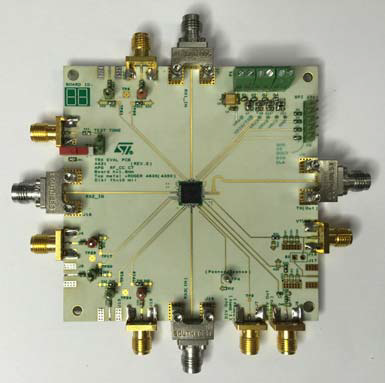
\includegraphics[max width=\hsize,max height=\maximheight,valign=t]{boards/img_ST.png}
\par\vspace{\extrarowheight}
\tabularnewline

OmniPreSense OPS241-A\footnote{\url{https://www.omnipresense.com/product/ops241-a/}}&
Arduino shield with BGT24LTR11&
24~GHz, 80~MHz &
On\nobreakdash-board, 1~Tx/Rx&
\$169&
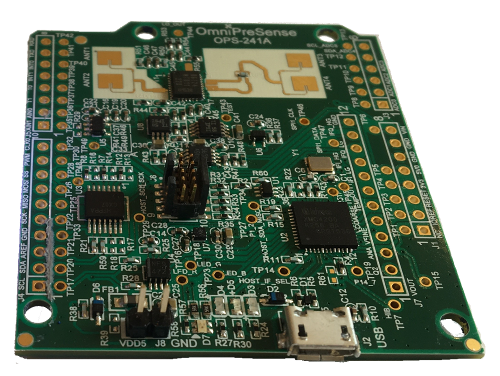
\includegraphics[max width=\hsize,max height=\maximheight,valign=t]{boards/img_omnipresense.png}
\par\vspace{\extrarowheight}
\tabularnewline

\bottomrule

\end{tabularx}

}


The antenna solutions are diverse. Some products provide only one antenna for transceiving, while others have up to 18 multiple-in-multiple-out (MIMO) antennas. A sufficient number of transmit antennas enables electronic beamforming, while enough receiving antennas provide DOA estimation capabilities. Some products require external antennas (and hence some additional design efforts), others with antennas integrated in the copper layer or in ceramic packages on the printed circuit board (PCB). Very interesting are also the radar sensors with antennas integrated in the integrated circuit's (IC) package or even silicon die. They miniaturize the product and take a lot of RF design work off the integrating engineer.

In the given time frame, the Walabot Pro, Omniradar RIC60-A and a proprietary Bosch prototype were available to be tested.

\subsubsection{Bosch Radar}\label{bosch-radar}

The Bosch radar presented some challenges under a Linux environment. After its Matlab driver was patched for cross-platform compatibility, it turned out that the on-board MCU's firmware had an incompatible protocol format. A newer version of the prototype that was later provided did work under Windows, but by the time the board arrived, the decision to focus on Omniradar's chip was made and the newer driver was not cross-plattform patched.

\subsubsection{Vayyar Walabot}\label{walabot}

Vayyar\footnote{\url{https://www.vayyar.com/}} is an Israeli
startup\footnote{\url{https://www.crunchbase.com/organization/vayyar}} that was founded in 2011. Coming from a medical background, they moved away from use cases such as breast cancer detection towards general 3D imaging in the consumer market with their Walabot sensor. Vayyar's Walabot Pro sensor uses an 18-antenna MIMO array for 3D radar imaging. Vayyar is very quiet about the technology and algorithms used in their product and even the nature of the data that the sensor sends.

In their Python \href{https://api.walabot.com}{API documentation} they showcase the available sensor operation modes: 3D imaging, 2D imaging, object tracking, pipe detection and raw data (see \cref{fig:walabot_image}).

\begin{figure}[htbp]
    \centering
    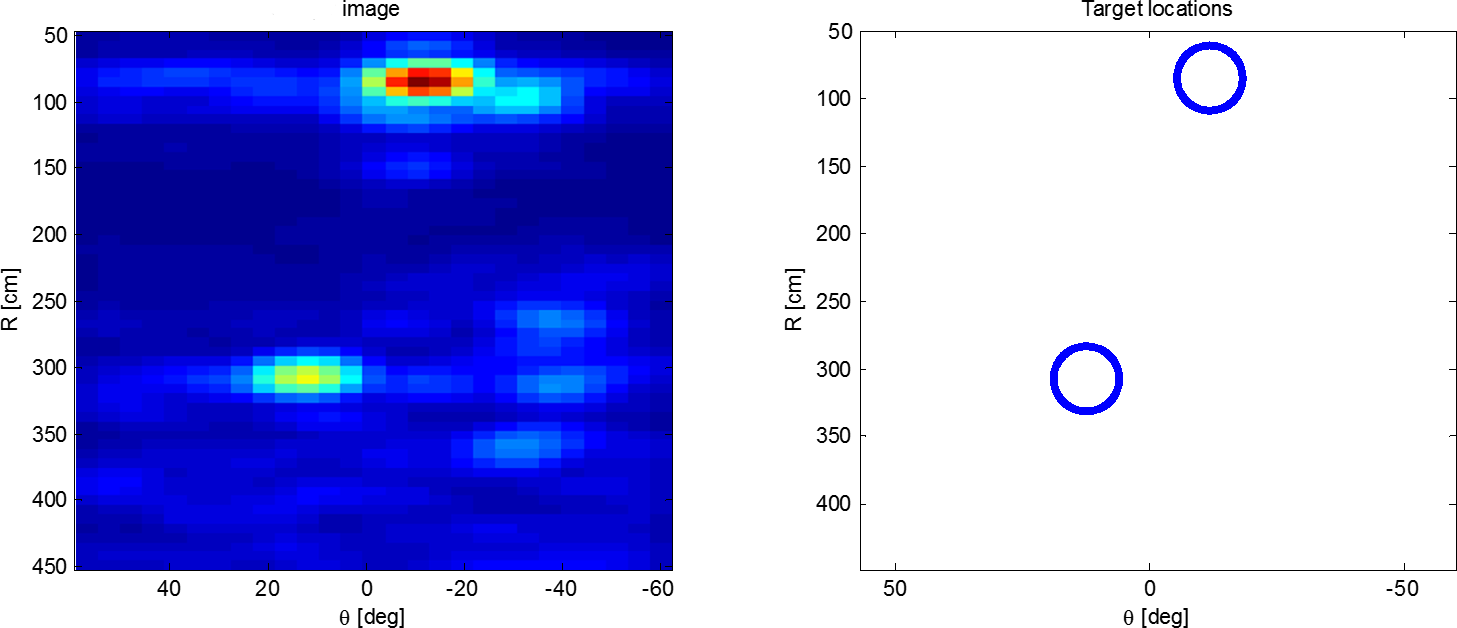
\includegraphics[max height=10cm,max width=10cm]{figures/walabot_image}
    \caption{Vayyar's Walabot Pro sensor is claimed to have Target localization and tracking. Source: \url{https://api.walabot.com/\_features.html\#\_examples}}
    \label{fig:walabot_image}
\end{figure}

The catch is that it is almost impossible to do imaging without background subtraction, which they do in all their examples. Granted, this works well in scenarios where the sensor is at a fixed position or if the region of interest is very small, like in the pipe detection scenario. However, In the case of a robot-mounted sensor this does not provide great data quality, because not only a small part, but the whole scene changes when the robot moves.

At the time of writing, the only interesting published project is a fall detection scenario \cite{Haider2017} by Haider, in which people can be localized at intersections of vertically and horizontally oriented heatmaps.

\subparagraph{Static range test}\label{static-range-test}

\Cref{fig:walabot_rangetest_data} shows the signal from two Walabot antenna pairs as it records the scene in image \cref{fig:walabot_rangetest_setup} with metal can stacks at \(0.5m\) \(1m\) and \(1.5m\). The signal is very stable over time and shows next to no noise. Unfortunately however it doesn't seem like the radar sensor can detect the metal cans at all. The high frequency signal is the raw signal as reported by the Walabot sensor. It is however hardly believable that it was measured like this, as the visible base frequency of the signal is around 7GHz. It was not possible to get any useful information from Vayyar's technical support regarding this. The envelope signal is a more interesting data source. It can easily be obtained from the analytic signal, using \texttt{scipy.signal}'s Hilbert transform.
Another problem with the data is that the peaks of the envelope jitter
in range. This can be fixed by combination with another oddity: The last
180 samples rise very strongly in magnitude. If they are cut and
prepended to the first sample, they match up perfectly. Peaks can then
be detected in the signal (represented by the dots \cref{fig:walabot_rangetest_data}) and
the range set to zero at the first peak. This eliminates the range
jitter completely. The reason is that the first peak is caused by
transmit antenna crosstalk and can thus be used as a timing reference
point.

\begin{figure}[htbp]
    \centering
    \begin{subfigure}{\textwidth}
        \centering
        \includegraphics[width=\linewidth]{pictures/experiment_walabot_rangetest}
        \caption{Setup with three towers of cans in front of the Walabot sensor}
        \label{fig:walabot_rangetest_setup}
    \end{subfigure}
    \begin{subfigure}{\textwidth}
        \centering
        \def\svgwidth{\linewidth}
        \input{gfx/fig_svg/walabot_rangetest.pdf_tex}
        \caption{Normalized echo intensity of range profile measurement with two antenna pairs. After the transmit peak at \(t=0\), three peaks corresponding to the three can targets are vaguely perceptible. }
        \label{fig:walabot_rangetest_data}
    \end{subfigure}
    \caption{Static range test with the Walabot sensor}
    \label{fig:walabot_rangetest}
\end{figure}

\subparagraph{Dynamic range test}\label{dynamic-range-test}

Waving hands in front of the sensor did give a change in signal, but it
was difficult to interpret the data conclusively. To objectively test
the sensor's response, an aluminum plate that gave a strong echo signal
was taped to the Kobuki robot. The robot was then driven with a constant
speed away from the sensor and then towards the sensor as pictured in
\cref{fig:walabot_dynamic_setup}.

The sensor was sampled at a constant frequency in raw data mode. The
analytic signal magnitude of the range scans is stacked at the right end of the
matrix displayed in \cref{fig:walabot_dynamic_data}.

\begin{figure}[htbp]
    \centering
    \subcaptionbox{Setup with a reflective metal plate mounted on the robot.}
        {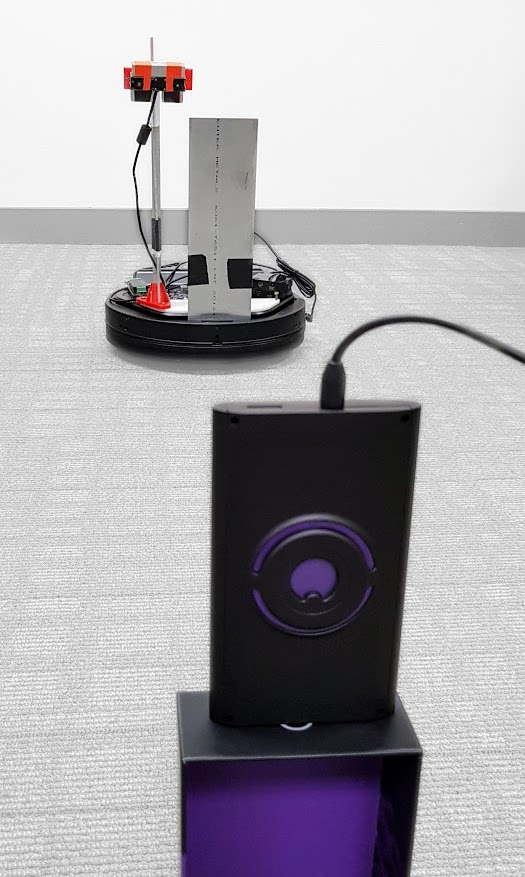
\includegraphics[max height=10cm,max width=10cm]{pictures/experiment_walabot}}
        \label{fig:walabot_dynamic_setup}
    \quad
    \subcaptionbox{Range profile (\textit{y-axis}) over time (\textit{x-axis}) while the robot was moved at constant speed away and towards the Walabot sensor.}
        {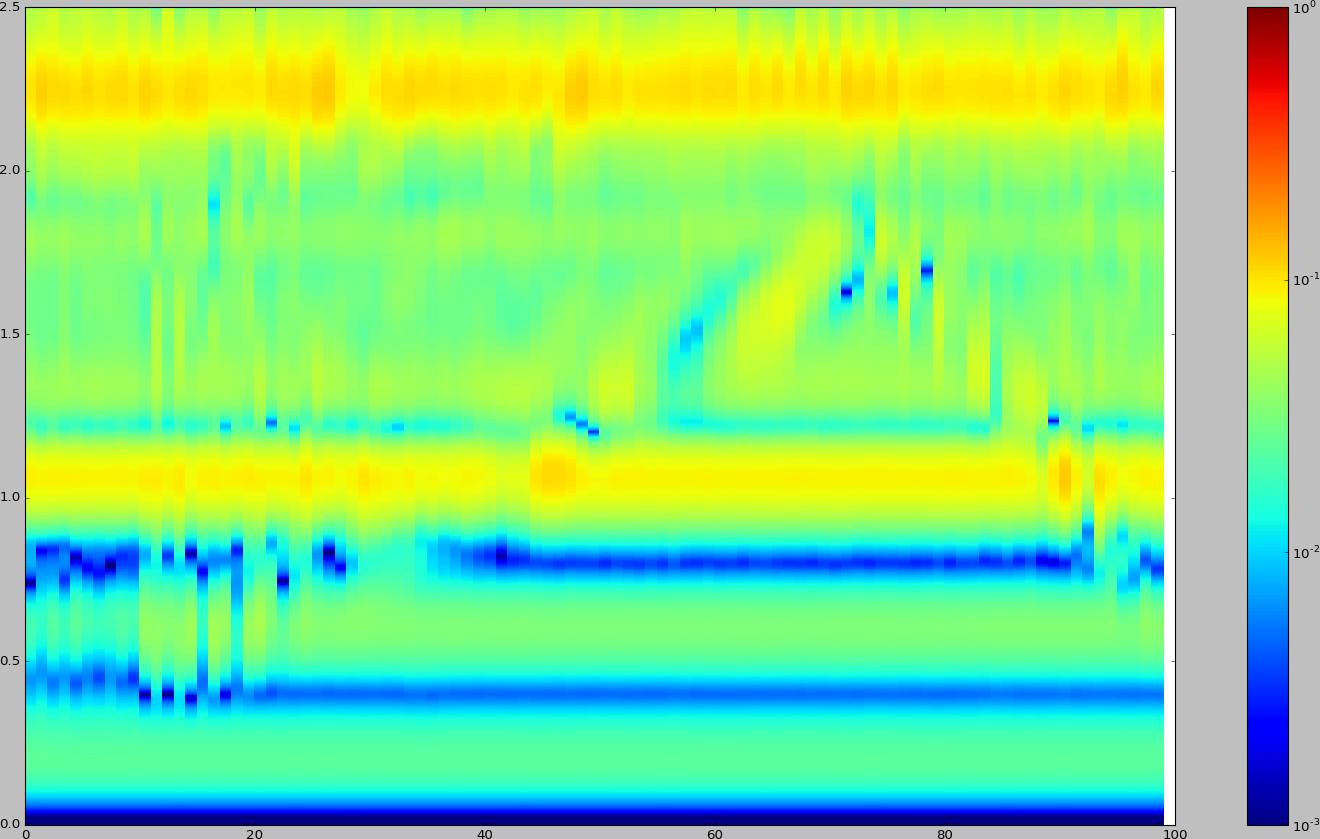
\includegraphics[max height=10cm,max width=10cm]{figures/walabot_disttest}}
        \label{fig:walabot_dynamic_data}
    \caption{Dynamic range test with the Walabot sensor}
\end{figure}

The figure shows that the Walabot has problems with what looks like
standing waves. The great amount of background signal is also visible.
Because of its static nature, this can easily removed for a fixed radar.
As some Walabot reviewers have noticed \cite{Valens2016} this background
signal changes heavily and seemingly random when the sensor is moved.
This makes the signal processing very difficult.

Walabot advertises object detection capabilities. The catch with this
mode is however that the number of objects to be detected must be
configured first.

\section{Omniradar RIC60-A}\label{omniradar}

With its good range resolution and a good idea of its capabilities from
\cite{Ernst2016}, this sensor promised good results. As it was chosen as
a basis for the proof of concept implementation, it receives a more
detailed look.

Founded in 2010, Omniradar\footnote{\url{https://www.omniradar.com/}} is a Dutch
startup\footnote{\url{https://www.crunchbase.com/organization/omniradar}} that
claims to be the first to integrate a complete 60 GHz radar including
antennas and analog to digital conversion in one chip.

With the RIC60-A they offer a Radar Development Kit (RDK) that gives
7GHz of bandwidth on two receiving antennas. An Altera Cyclone IV FPGA
handles the signal acquisition and communication. \Cref{fig:slide_RIC60A} shows the
radar IC and how the three antennas are integrated in silicon.

\begin{figure}[htbp]
    \centering
    \def\svgwidth{\linewidth}
    \input{gfx/pictures/slide_RIC60A.pdf_tex}
    \caption{Decapped Omniradar IC; five cent coin as size reference; and antenna directionality pattern of Omniradar's RIC60-A. Source: \cite{Brouwer2015} p.9}
    \label{fig:slide_RIC60A}
\end{figure}

The radar sensor's beam is fan shaped, which means it is fairly
sensitive over a wide angle in azimuth direction, but relatively focused
in elevation. This makes it a very good candidate for the radar
reprojection, as targets can be seen from the robot in a wide field of
view, but floor and ceiling reflections are kept at a minimum. Of course
the sensor can also be rotated. Omniradar also supplies a horn-like
extension for the sensor board, which forms the radar sensitivity into a
pencil-shaped beam that is very focused at a narrow field of view.

\begin{figure}[htbp]
    \centering
    \begin{subfigure}[b]{0.45\textwidth}
        \label{fig:omniradar}
        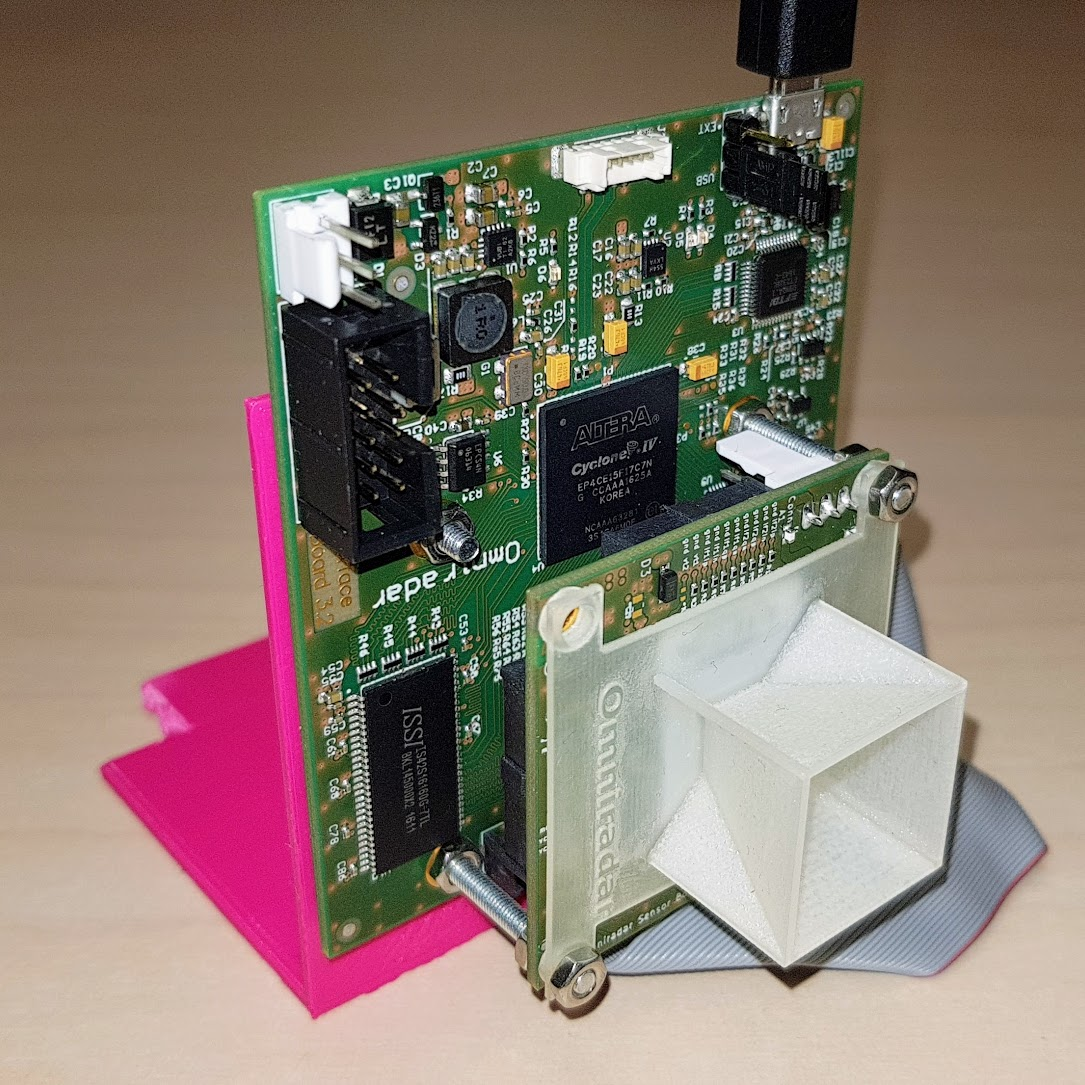
\includegraphics[max width=\linewidth]{pictures/omniradar}
        \caption{Omniradar's RIC60-A sensor with horn antenna extension, attached to the 3D-printed Kobuki mount}
    \end{subfigure}
    \hfill
    \begin{subfigure}[b]{0.45\textwidth}
        \centering
        \label{fig:mount}
        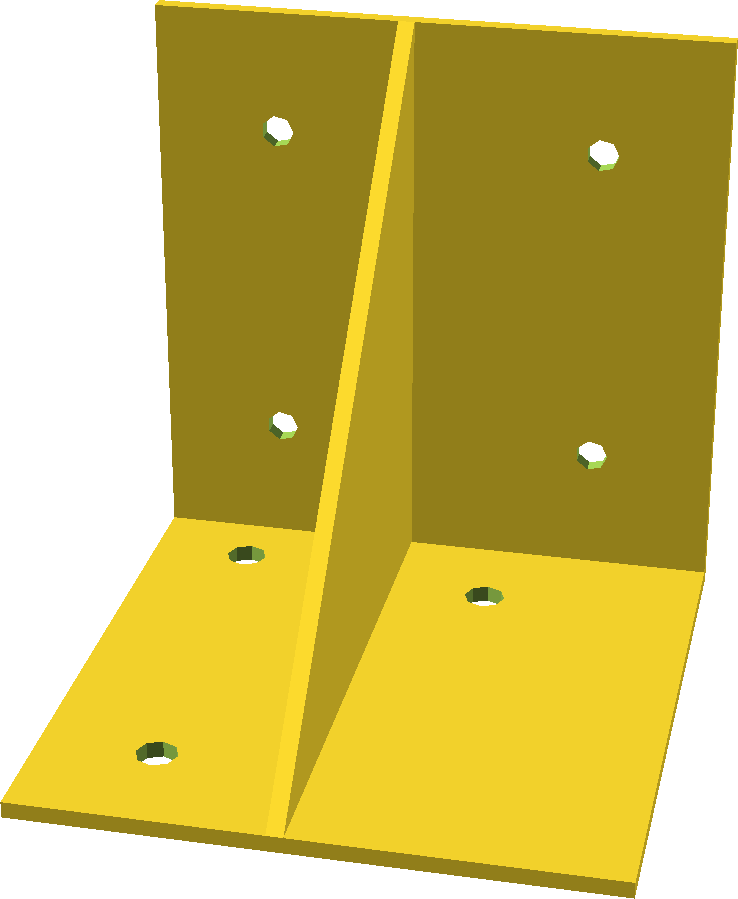
\includegraphics[max width=\linewidth]{models/mount.png}
        \caption{3D model of the radar sensor mount, designed with OpenSCAD.\bigskip}
    \end{subfigure}
    \caption{Radar sensor on mount and model of the mount.}
\end{figure}


\subsection{Radar mount}\label{radar-mount}

A 3D-printed part makes sure that the radar sensor is firmly mounted on
the robot as it explores its environment. The part was designed in
\href{http://www.openscad.org/}{OpenSCAD} and printed on a
\href{https://3dprinter.dremel.com/}{Dremel 3D printer}. The bottom
mount hole positions were extracted from the mechanical drawings of the
Kobuki Base \cite{YujinRobot2012}; the side holes from the Altium layer
document of the version 3.2 Omniradar interface board
\cite{Omniradar2014}.

When rotated to face to the left side of the robot, the RPLidar mount
was in the way, so parts of the print had to be clipped off.

Two screws hold the Omniradar interface board to the mount. The other
two mounting holes in the interface board hold the Omniradar sensor
board. The horn extension can be affixed to these screws as well. If a
different sensor orientation is necessary, the sensor board can be
rotated by 90 degrees, thanks to the symmetric layout.

\subsection{Doppler sensitivity}\label{doppler-sensitivity}

The Omniradar FMCW radar is not sensitive enough to use the Doppler
speed directly. The following example illustrates this.

The RIC60A has a sensitivity of \(400 \frac{Hz}{m/s}\). A target with a
doppler speed of \(0.02 m/s\) (A low speed at which the Kobuki robot
still moves continuously and without jerking) will cause a frequency
spike with a shift of \(8Hz\) in the FMCW beat frequency.

The speed resolution capability is inversely proportional to the
measurement or acquisition time. A 10 ms long acquisition gives a 100 Hz
frequency resolution, or a speed resolution of 0.9 km/h (or 0.25 m/s).

Sampling frequency \(F_s=25MHz\) and RIC60A Doppler sensitivity,
\(S_D = 400 \frac{Hz}{m/s}\) are constant values of the Omniradar RDK.

Given a chirp duration of \(T_{chirp} = 2.5ms\), we get
\(N_s = t_{chirp} F_s = 62500\) Samples,
\(N_r = \lfloor \frac{N_s}{2} \rfloor = 31250\) Samples per
up/downsweep, \(dF = \frac{F_s}{N_r - 1} = 800 Hz\) FFT frequency bin
width and hence a Doppler resolution of \(\frac{dF}{S_D} = 2 m/s\).

Even with subsample peak interpolation the accuracy will not be very
good and targets will be reprojected at imprecise angles.

It would be possible to use higher precision equipment. But another
solution is to track the movement of target peaks in the range profile,
using the Peak Gradient algorithm.

\subsection{Optimal chirp time configuration}\label{optimal-chirp-time-configuration}

The chirp duration \(t_{chirp}\) is configurable and has an effect on
how the raw range profile data will look like.

\textbf{Very short durations} (\(<2ms\)) incur a considerable processing
overhead to acquisition time ratio and have a very low SNR.\\
\textbf{Short durations} (\(<5ms\)) have acceptable SNR, and are more
efficient with respect to overhead.\\
\textbf{Long durations} (\(>15ms\))
have good SNR, and don't create a lot of overhead. However at higher
robot speeds, target peaks get blurred over several range bins as they
move in range. Less intense target echos are more difficult to detect
then.\\
\textbf{Very long durations} (\(>20ms\)) required the Omniradar
driver to be patched on Linux so as not to freeze when chirps longer
than \(20ms\) are requested. Even with the patched driver the RDK's FPGA
firmware is not very reliable at sending large volumes of data at once
and corrupts packet headers or aborts transmissions intermittently.

The optimal range was empirically found to lie between \(2ms\) and
\(10ms\).

TODO wording here

\Cref{fig:fig_chirp_eff} shows the chirp efficiency
\(\eta = \frac{n_{chirp}~t_{chirp}}{t_{msg}}\), with number of
consecutive sweeps \(n_{chirp}\) (two in the graph's data source), chirp
length \(t_{chirp}\), and \(t_{msg}\) the time since last radar message.

\begin{figure}[htbp]
    \centering
    \def\svgwidth{10cm}
    \input{gfx/fig_svg/chirp_eff.pdf_tex}
    \caption{Chirp efficiency \(\eta\) (measurement time per time spent) for various chirp lengths}
    \label{fig:fig_chirp_eff}
\end{figure}

The chirp length has an effect on accuracy and resolution. \Cref{fig:fig_compare_chirp_times} shows the range profiles of one scene, recorded over $10s$. Short chirp times lead to a higher noise floor, but exhibit less variance, i.e. a slimmer band of frequencies. Longer measurement times have a lower noise floor but have more outliers. Especially with the horn extension attached longer measurement time also improves SNR.

\begin{figure}[htbp]
    \centering
    \begin{subfigure}{0.475 \textwidth}
        \centering
        \def\svgwidth{\linewidth} \small
        \input{gfx/fig_svg/chirp_comp_2.pdf_tex}
        \caption{Normalized echo intensity of range profiles without horn extension}
        \bigskip
    \end{subfigure}
    \hfill
    \begin{subfigure}{0.475 \textwidth}
        \centering
        \def\svgwidth{\linewidth} \small
        \input{gfx/fig_svg/chirp_comp_1.pdf_tex}
        \caption{Normalized echo intensity of range profiles with horn extension}
        \bigskip
    \end{subfigure}
    \begin{subfigure}{0.475 \textwidth}
        \centering
        \def\svgwidth{\linewidth} \small
        \input{gfx/fig_svg/chirp_comp_4.pdf_tex}
        \caption{Normalized harmonic mean of range profiles, without horn extension}
    \end{subfigure}
    \hfill
    \begin{subfigure}{0.475 \textwidth}
        \centering
        \def\svgwidth{\linewidth} \small
        \input{gfx/fig_svg/chirp_comp_3.pdf_tex}
        \caption{Normalized harmonic mean of range profiles, with horn extension}
    \end{subfigure}
    \caption{Effect of chirp length on SNR; with and without Horn extension}
    \label{fig:fig_compare_chirp_times}
\end{figure}


\section{Omniradar ROS driver}\label{omniradar-ros-driver}

The Omniradar RIC60A comes with a precompiled Matlab MEX driver library.
This works well in a Windows OS on x86-based computers with a Matlab
installation. An early goal was to have the robot carry the radar module
around wireless. One option would have been to mount a Windows laptop on
the Kobuki. However, Omniradar was kind enough to provide the author
with the driver sources under an NDA agreement. This allowed recompiling
the MEX driver for Linux systems. There were some issues with FTDI's
D2XX serial communication library that had to be fixed for Linux
systems. One challenge with the D2XX driver was that Ubuntu
automatically loads the regular FTDI serial IO driver,
\texttt{ftdi\_sio}. This was be solved by unbinding the driver using a
set of udev rules \footnote{\url{https://stackoverflow.com/questions/44529376}}. Another
issue was that due to a bug in the D2XX implementation, the Omniradar
driver would freeze when more than 2MB of data (equivalent to a 20ms
FMCW chirp) were requested. After a lot of debugging, this could be
solved by never requesting a bigger amount of data than was already
available in the D2XX buffer.

\subsection{C++ bindings and library}\label{c-bindings-and-library}

Since Matlab does not run on Arm arch processors such as the Odroid on
the Kobuki robot, a new set of platform-independent C++ bindings was
added to the driver. The C++ bindings serve the same purpose as the
Matlab bindings.

To include the library, some files need to be installed or pointed to by
the binary that needs to use it.

{ \rowcolors{1}{}{ColorAlternatedRow}
\begin{tabularx}{\textwidth}
{%
  >{\setlength{\hsize}{.25\hsize}\raggedright\arraybackslash}X%
  >{\setlength{\hsize}{.325\hsize}\raggedright\arraybackslash}X%
  >{\setlength{\hsize}{.425\hsize}}X%
}
\hiderowcolors
  File &
  Default install destination &
  Purpose \\
\midrule
\endhead
\showrowcolors

omniradar.h &
/usr/local/include &
Library header file \\

libomniradar.so &
/usr/local/lib &
dynamically linked shared object \\

51-omniradar.rules, 52-omniradar.rules &
/etc/udev/rules.d/ &
Udev rules to unbind ftdi\_sio \\
\bottomrule
\end{tabularx}
} % rowcolors
If the driver source is available, installing the files can be
accomplished from the source directory with

\begin{Shaded}
\begin{Highlighting}[]
\FunctionTok{mkdir}\NormalTok{ build }\KeywordTok{\&\&} \BuiltInTok{cd}\NormalTok{ build}
\FunctionTok{cmake}\NormalTok{ -DCPP_BINDINGS=ON -DMATLAB_BINDINGS=OFF ..}
\FunctionTok{make}
\FunctionTok{sudo}\NormalTok{ make install}
\end{Highlighting}
\end{Shaded}

The driver can then be included in an application. Note that since it is
dynamically linked, the \texttt{ftd2xx}, \texttt{pthread} and
\texttt{dl} libraries dependencies also need to be linked. In a Catkin
\footnote{Catkin is the CMake-based ROS build system} CMakeLists.txt
this would look like

\begin{Shaded}
\begin{Highlighting}[]
\KeywordTok{target_link_libraries}\NormalTok{(}
  \VariableTok{\$\{PROJECT_NAME\}}\NormalTok{_node}
\NormalTok{  omniradar}
\NormalTok{  ftd2xx}
\NormalTok{  pthread}
\NormalTok{  dl}
  \VariableTok{\$\{catkin_LIBRARIES\}}
\NormalTok{)}
\end{Highlighting}
\end{Shaded}

The C++ library offers the same functions as Omniradar's Matlab driver,
with two differences. The optional device index number is 0-based
instead of 1-based and the AquireEcho functions return (a shared pointer
to) packed data instead of unpacked data for performance reasons. With
the

\begin{Shaded}
\begin{Highlighting}[]
\AttributeTok{static} \BuiltInTok{std::}\NormalTok{shared_ptr< }\BuiltInTok{std::}\NormalTok{vector< }\BuiltInTok{std::}\NormalTok{vector< }\DataTypeTok{uint8_t}\NormalTok{ > > >}\\
\NormalTok{    demultiplex(}\BuiltInTok{std::}\NormalTok{vector<}\DataTypeTok{uint32_t}\NormalTok{> \&packed_data);}
\end{Highlighting}
\end{Shaded}

function, the library offers an easy way to demultiplex the packed data
array into a (shared pointer to a) vector of four vectors - one for each
echo signal of the I/Q channel of left and right receiving antenna.

Useage is simple as the driver follows the RAII principle. Allocation of
an object of type \texttt{Omniradar} causes the library to fully
initialize the RIC60A RDK. After that, the configuration string and the
VCO tuning curve should be set. Omniradar provides some Matlab example
code that measures the sensor's VCO tuning curve. The easiest way to
bring this tuning curve into the C++ domain is to
print\footnote{`['A' 10 'B']` is a quick way to print a newline character between `A` and `B`}
it as C style array, e.g.~with

\begin{Shaded}
\begin{Highlighting}[]
\NormalTok{[ }\StringTok{'#pragma once'} \FloatTok{10} \StringTok{'std::vector<double>'} \FloatTok{10} \KeywordTok{...}\\
\NormalTok{    }\StringTok{'vco_tune \{'}\NormalTok{, sprintf(}\StringTok{'\%.100g, '}\NormalTok{, VCOtune), }\StringTok{'\};'}\NormalTok{ ]}
\end{Highlighting}
\end{Shaded}

and then saving the resulting string as \texttt{vco\_tune.h} include
file.

This setup allowed the development of a ROS node that handles
communication with the radar module on the Linux/Arm based Kobuki robot.

\subsection{ROS node}\label{ros-node}

A new \texttt{omniradar} ROS package was developed to support the use of
the Omniradar sensor within the ROS environment. A set of
\texttt{roslaunch} launchfiles comes with the package that support the
startup of the Kobuki robot in teleoperation mode, optionally together
with lidar-based Cartographer slam, AMCL localization and an Astra
Orbbec RGBD camera. A simple version to start the only the node to get
radar data would be:

\begin{Shaded}
\begin{Highlighting}[]
\NormalTok{<launch>}\\
\NormalTok{  <node }\AttributeTok{pkg=} \StringTok{"omniradar"} \AttributeTok{type=} \StringTok{"omniradar_node"} \AttributeTok{name=}\StringTok{"omniradar_node"}\\
\NormalTok{    }\AttributeTok{output=}\StringTok{"screen"}\NormalTok{>}\\
\NormalTok{    <param }\AttributeTok{name=}\StringTok{"n_sweeps"} \AttributeTok{value=}"1"\NormalTok{ />}\\
\NormalTok{    <param }\AttributeTok{name=}\StringTok{"t_sweep"}  \AttributeTok{value=}"5"\NormalTok{ />}\\
\NormalTok{  </node>}\\
\NormalTok{</launch>}
\end{Highlighting}
\end{Shaded}

The node sends out the ROS topic \texttt{/omniradar\_node/radar\_raw} of
the custom \texttt{RadarEcho} type, which is defined in RadarEcho.msg as

\begin{Shaded}
\begin{Highlighting}[]
\DataTypeTok{Header} header
\DataTypeTok{string} ric_config
\DataTypeTok{uint8} n_sweeps
\DataTypeTok{float64} t_sweep
\DataTypeTok{uint32[]} packed_echo
\end{Highlighting}
\end{Shaded}


Early versions of the driver unpacked the radar echo bitstream inside
the node and were able to use standard ROS message types like the
\texttt{std\_msgs/ByteMultiArray} message. However, sending out the
packed bitstream proved to be much more efficient in terms of chirp
efficiency \(\eta\). The custom message type also allows to send out the
configuration (RIC configuration string, number and length of FMCW
sweeps) that was used to attain the message's echo. The message's
timestamp and sequential ID is contained in the regular
\texttt{std\_msgs/Header}.

\begin{figure}[htbp]
    \centering
    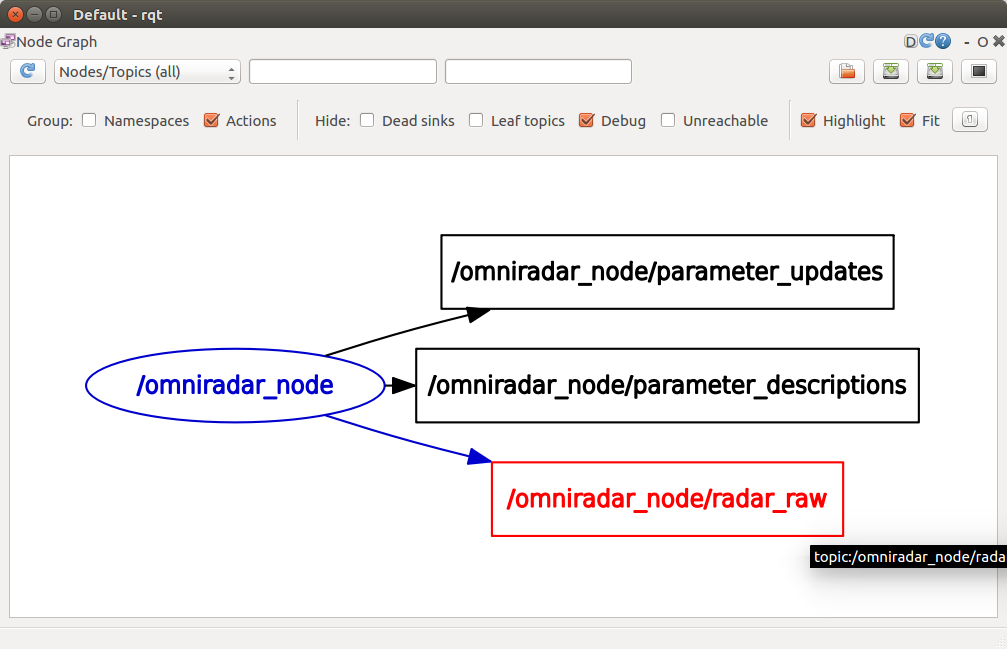
\includegraphics[max height=10cm,max width=10cm]{screenshots/nodegraph}
    \caption{Omniradar rosnode node graph with leaf topics}
    \label{fig:nodegraph}
\end{figure}

While parameters from the ROS parameter server (as configured in the
launch) are respected, the node also offers a dynamic reconfigure server
to change RIC configuration string, number of sweeps and length of sweep
on the fly without the need to restart the node (see \cref{fig:dynreconf}).

\begin{figure}[htbp]
    \centering
    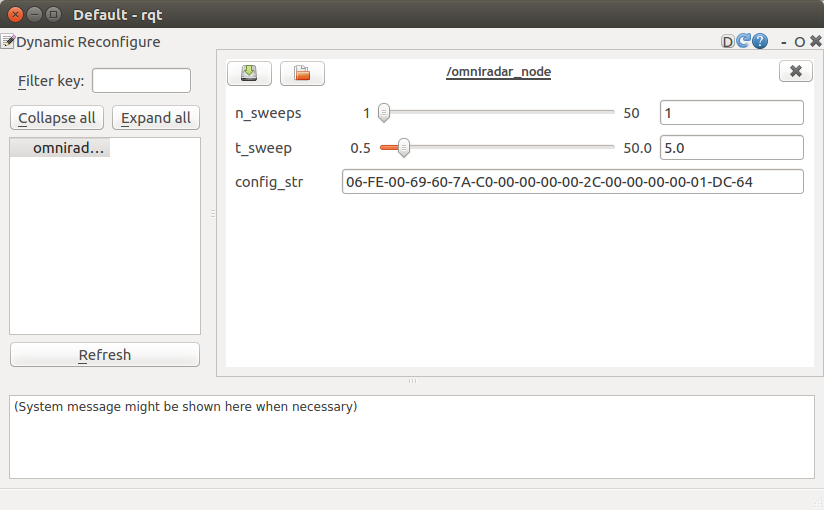
\includegraphics[max height=10cm,max width=10cm]{screenshots/dynreconf}
    \caption{Dynamic reconfigure options for the Omniradar rosnode}
    \label{fig:dynreconf}
\end{figure}

The core of the node is a while loop that continuously triggers radar
echo acquisition and copies the result into a new
\texttt{omniradar::RadarEcho} message. The radar sensor update rate
could be increased by offloading the message assembly and data copying
into a C++11 lambda thread that is immediately detached.

\begin{samepage}
\begin{Shaded}
\begin{Highlighting}[]
\BuiltInTok{std::}\NormalTok{lock_guard<}\BuiltInTok{std::}\NormalTok{mutex> lock_rdk(mtx_rdk);}
\KeywordTok{auto}\NormalTok{ t_echo = ros::Time::now();}
\KeywordTok{auto}\NormalTok{ p_echo = rdk->AcquireEcho(msg.n_sweeps);}

\BuiltInTok{std::}\NormalTok{thread t (}
\NormalTok{    [=] ()}
\NormalTok{    \{}
        \BuiltInTok{std::}\NormalTok{lock_guard<}\BuiltInTok{std::}\NormalTok{mutex> lock_msg(mtx_msg);}
\NormalTok{        msg.header.stamp = t_echo;}
\NormalTok{        msg.packed_echo.resize(p_echo->size());}
        \BuiltInTok{std::}\NormalTok{copy(p_echo->begin(), p_echo->end(), msg.packed_echo.begin());}
\NormalTok{        pub.publish(msg);}
\NormalTok{        msg.header.seq++;}
\NormalTok{    \}}
\NormalTok{);}
\NormalTok{t.detach();}
\end{Highlighting}
\end{Shaded}
\end{samepage}

The multithreading approach lets the node use between 100\% and 140\%
CPU (observed with \texttt{htop}).

\section{Matlab}\label{matlab}

Matlab (release R2017a) was chosen as implementation platform and
language because it allows quick prototyping, provides relatively easy
visualization, and, with the Robotics Toolbox, supports many ROS
features.

\subsection{Custom ROS message
support}\label{custom-ros-message-support}

It is necessary to install custom message support with the
\href{https://www.mathworks.com/help/robotics/ref/roboticsaddons.html}{roboticsAddon}
and
\href{https://www.mathworks.com/help/robotics/ug/create-custom-messages-from-ros-package.html}{generate}
the files to read in rosbags with \texttt{RadarEcho} type messages.

\section{Complementing sensors}\label{complementing-sensors}

TODO

\subsection{RGBD}\label{rgbd}

\subsection{Lidar}\label{lidar}

\section{Implementation}\label{implementation-1}

\subsection{Overview}\label{overview}

\subsection{Data path}\label{data-path}

\subsection{Code structure}\label{code-structure}

\subsection{Usage}\label{usage}

\begin{enumerate}
\def\labelenumi{\arabic{enumi}.}
\tightlist
\item
  Start robot, connect three sessions with \texttt{ssh\ zero2-pa}
\item
  Start ROS core with \texttt{roscore}
\item
  Start the node, with keyboard teleoperation and Cartographer Laser
  Slam:
  \texttt{roslaunch\ omniradar\ omniradar\_teleop\_lidarslam.launch}
\item
  Use \texttt{rqt} with the \emph{Dynamic Reconfigure} plugin to set the
  Omniradar node to generate the preferred number of sweeps and sweep
  duration. The configuration string can also be changed. The defaults
  are fine (One 5ms sweep)
\item
  \texttt{rosbag\ record\ /omniradar\_node/radar\_raw\ /odom\ /tf\ /map\ -O\ scan}
  will record a rosbag ``scan.bag'' containing all ROS messages with
  radar data, Kobuki odometry and slam map and transforms from
  Cartographer.
\item
  In the terminal running \texttt{roslaunch}, use the arrow keys to move
  the robot around (\(\uparrow\) and \(\downarrow\) to increase and
  decrease speed, \(\leftarrow\) and \(\rightarrow\) to increase and
  decrease rotation speed). \(E\) resets speed to zero and makes the
  robot halt.
\item
  After recording some interesting data, stop the rosbag record
  (\(Ctrl+C\)). Open a new terminal on your local machine and run
  \texttt{ssh\ zero2-pa\ "tar\ zcf\ -\ scan.bag"\ \textbar{}\ tar\ zxf\ -}.
  The rosbag will be transferred to your machine. Using ssh with the tar
  pipe is the fastest way to transfer the data (around \(100 Mbps\) on
  the BSH wifi). Compressing first (\texttt{rosbag\ compress\ scan.bag})
  and then sending takes a while on the not-so-powerful Odroid platform.
\item
  Optionally filter out unwanted transforms from the rosbag to speed up
  later processing:
  \texttt{rosbag\ filter\ scan.bag\ scan\_filtered.bag\ \textquotesingle{}(topic\ ==\ "/tf"\ and\ m.transforms{[}0{]}.child\_frame\_id\ ==\ "odom")\ or\ topic\ !=\ "/tf"\textquotesingle{}}
\item
  In Matlab, run
  \texttt{radar\_data\ =\ radar\_bag2array("/path/to/your/scan.bag");}.
  This will read the bag sequentially into memory and extract the data:
  The robot position is recorded from odometry information and corrected
  using the /map \(\rightarrow\) /odom transform as reported by slam
  localization. Cross range mileage is calculated as cumulative sum of
  distance between radar positions (as the radar is not mounted over the
  robot's rotation center, the radar mileage is different from robot
  mileage as soon as any rotational velocity is present). Lastly, all
  values are interpolated at the radar message timestamps. It is a good
  idea to save the function's output, using
  \texttt{save(\textquotesingle{}radar\_data/radar\_data\_scan.mat\textquotesingle{},\ \textquotesingle{}radar\_data\textquotesingle{})}
\item
  The radar data can now be analyzed. The
  \texttt{plot\_world\_projection} script can be used to get a good
  overview over raw data, doppler speeds, direction of arrival, and
  reprojection map.
\item
  To compare radar reprojection map and laser slam map, try the
  \texttt{test\_slam\_overlay} with the correct bag filename (the lidar
  map is extracted from that bag)
\end{enumerate}

\section{Data Preprocessing}\label{data-preprocessing}

TODO

\subsection{Rosbag to Matlab}\label{rosbag-to-matlab}

\subsection{(Odometry) Cross range
interpolation}\label{odometry-cross-range-interpolation}

\subsection{Raw Data Smoothing}\label{raw-data-smoothing}

After taking a single range reading, it will usually be relatively
noisy. One solution to getting cleaner range data with higher SNR is
oversampling. It is possible to use a moving average over a certain
accumulation distance to achieve this. However, the number of raw
samples is quite high and processing each sample takes a considerable
amount of time (some minutes for some minutes of recorded data). It is
better to make use of binning, with bins the width of the accumulation
distance. All samples in one bin are averaged to represent that bin's
value. This greatly improves processing time (to less than a second for
some minutes of recorded data).

\Cref{fig:fig_compare_means} shows in gray the raw data of the first 20 range scan lines
from the ``Mancave'' dataset. It then compares different ways of
averaging over these 20 scans. All of them increase the SNR, because a
big part of the noise signal is statistically uncorrelated. Table \cref{tab:mean}
compares the RMS of the difference of each signal to the harmonic mean,
which gives the cleanest signal.

\begin{table}[htbp]
\rowcolors{1}{ColorAlternatedRow}{}
\begin{tabularx}{0.5\textwidth}{XX}
\hiderowcolors
\toprule
Signal & RMS of difference to harmonic mean\tabularnewline
\midrule
\endhead
\showrowcolors
Harmonic mean & 0\tabularnewline
Geometric mean & 0.144\tabularnewline
Arithmetic mean & 0.275\tabularnewline
50\%-Trim mean & 0.284\tabularnewline
Median & 0.318\tabularnewline
Raw & 1.064\tabularnewline
\bottomrule
\end{tabularx}
\caption{Comparison of mean types by RMS}
\label{tab:mean}
\end{table}

The harmonic mean is defined as
\[harmmean(x_{1,2,...,n}) = \frac{n}{\frac1{x_1} + \frac1{x_2} + \cdots + \frac1{x_n}} = \frac{n}{\sum\limits_{i=1}^n \frac1{x_i}}\]
The geometric mean is defined as
\[geomean(x_{1,2,...,n}) = \left(\prod_{i=1}^n x_i \right)^\frac{1}{n} = \sqrt[n]{x_1 x_2 \cdots x_n}.\]
The arithmetic mean is defined as
\[mean(x_{1,2,...,n}) = \frac{1}{n}\sum_{i=1}^n x_i=\frac{x_1+x_2+\cdots+x_n}{n}\]
The 50\% trimmed mean is defined as the arithmetic mean of all except
the highest and lowest \(\frac{n}4\) data points, where \(n\) is the
number of data points. The median is defined as the value that lies
between the lower and the upper half of sample values.

\begin{figure}[htbp]
    \centering
    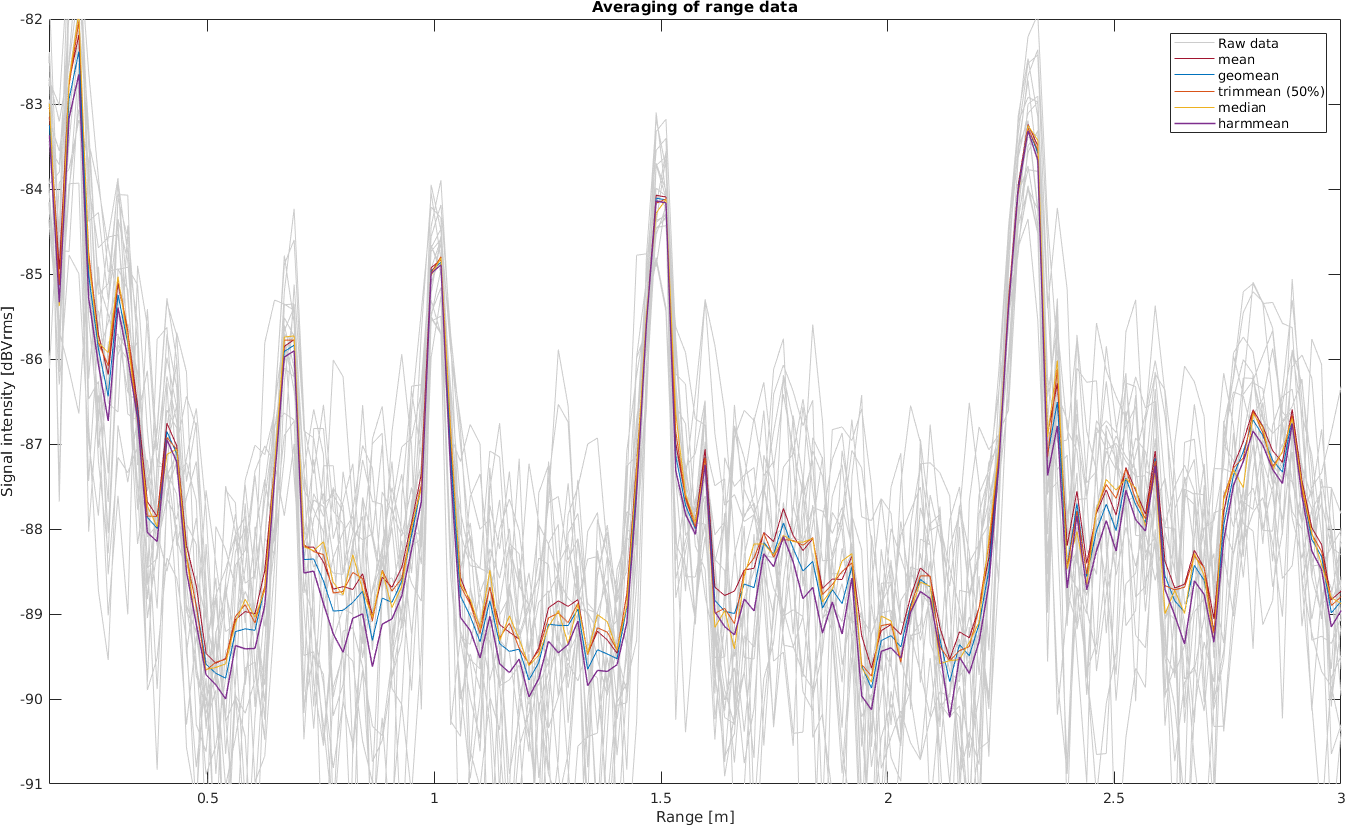
\includegraphics[max height=10cm,max width=10cm]{figures/fig_compare_means}
    \caption{Range profile quality comparison with different averaging functions. Higher peak-to-trough ratio is better.}
    \label{fig:fig_compare_means}
\end{figure}

Due to the good signal quality, the implementation uses the harmonic
mean to average the bins. Weighting the average with triangular or
Gauss-shaped weight distribution did not noticeably improve data quality
for any of the averaging methods.

Note that the range signal is not the only signal that needs to be
averaged in a range bin. All other parameters that are part of the range
scan need to be averaged as well. These parameters are mileage at scan
time, robot position and orientation, and robot speed. Sweep time and
down range bins don't change.

\section{Doppler Estimation with the Peak Gradient Algorithm}\label{doppler-estimation-with-the-peak-gradient-algorithm}

The peak gradient algorithm is a way to find Doppler speeds from
consecutive range profiles.

TODO subfigures, adjust references

\begin{figure}[htbp]
    \centering
    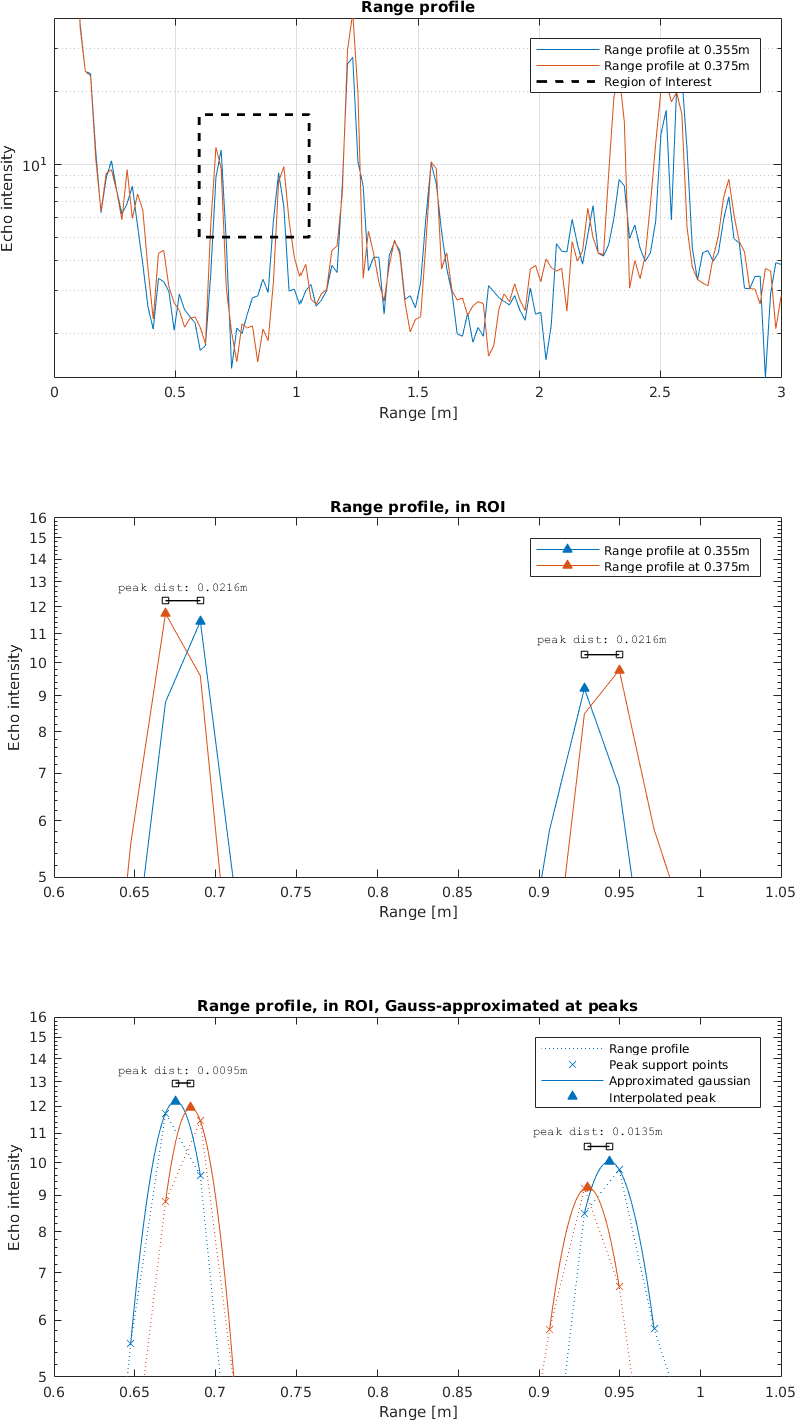
\includegraphics[max height=10cm,max width=10cm]{figures/fig_explain_peak_gradient.png}
    \caption{Peak detection and subsample peak interpolation to find peak distance between two range profiles}
    \label{fig:fig_explain_peak_gradient}
\end{figure}

In \cref{fig:fig_explain_peak_gradient} the scans at radar mileage \(0.355m\) and \(0.375m\) of
a scene (``Basement'') are overlaid. Obviously the range profiles of the
two scans are very similar. However, as visible in \cref{fig:fig_explain_peak_gradient} some
peaks from target echoes are shifted, as the distance to the targets
changes with the radar moving through the scene. The rate at which the
distance to a target changes is its relative speed to the radar, the
Doppler speed.

Usually, speed is measured in distance per time. In this case, it
actually makes sense to ignore the scan's time stamps and look at the
cross range (driven mileage) instead. With the Doppler speed as change
of down range (distance to target) per cross range driven, calculations
become time independent and hence radar movement speed independent.

A target's distance from the radar is assumed to be at the range bin of
the corresponding peak in a scan's range profile. When a target's
distance changes the peak will shift, too. This is visible in \cref{fig:fig_explain_peak_gradient} and we can read the Doppler speed from the figure. The peak around
\(0.67m\) moves \(d_{down,1} = 0.0216m\) closer in range, while the peak
around \(0.95m\) moves \(d_{down,2} = -0.0216m\) closer (i.e., away).
Combined with the change in cross range,
\(d_{cross} = 0.3752m - 0.3555m = 0.0197m\), we can calculate Doppler
speeds of \(v_{D,1} = \frac{d_{down,1}}{d_{cross}} = 109.55 \%\) (of
radar movement speed) and
\(v_{D,2} = \frac{d_{down,2}}{d_{cross}} = -109.55 \%\). If the speeds
were \(100\%\) and \(-100\%\) it would mean that the targets are directly
ahead and directly behind the moving radar. Speeds over 100\% are
however impossible in a static environment where all relative target
motion is caused by the radar movement. The targets are therefore either
dynamic and moving by themselves, or the peak locations that determined
those too-high speeds were not exact. Since we know that there were no
dynamic moving objects in the controlled environment of the scan, the
latter must be the case.

This effect of imprecise target peak localization and Doppler speed
estimation could be overcome by averaging noisy data so that the average
peak distance is close to the actual change in target range. A lot more
scans are necessary for that though, and scan oversampling needs to be
drastically reduced. This would lead to lower SNR, which means that some
peaks with lower echo intensity could not be detected.

With higher downrange resolution, peaks could be localized more
precisely. However, the down range resolution is limited by the
available bandwidth of the radar sensor. In the Omniradar RIC60A, up to
7GHz are available, which is already extremely high. Its range
resolution \(dR\) is \(\frac{c}{2 BW}\), which is roughly \(2.1cm\). With
this method, \(dR\) is of course the smallest measurable change of
target range.

The localization of peaks is however not limited by range resolution,
but by range accuracy, which mainly depends on SNR. It is much better
than range resolution with \(\sigma_R = \frac{dR}{\sqrt{SNR}}\). This
can be utilized with subsample peak interpolation.

\subsection{Inter-scan vs Intra-scan Doppler estimation}\label{inter-scan-vs-intra-scan-doppler-estimation}

For correct Doppler estimation it is important to have the exact timing,
or for relative Doppler speed, exact cross range mileage of the range
scans whose peaks are compared in the peak gradient algorithm.

The Omniradar sensor can send multiple consecutive sweeps without any
delay between them. The timing will then be very exact, because the
precise length of one sweep is known. However, the number of sweeps in
such a set of sweeps is limited (transmission of high data volumes will
often fail), so they can't be average to be smoothed through
oversampling and will be noisy. Smaller peaks will then not be detected
reliably. Another problem with this approach is that it will give target
Doppler speeds in change of down range over time, but not the robot
speed-invariant relative Doppler speed in change of down range over
change of cross range.

Inter-scan comparison gives better Doppler estimation, because the data
can be smoothed through oversampling first. Consecutive sweeps can still
be used: They need to be separated into individual scans with timestamps
adjusted to \(t_{msg} + i\cdot t_{sweep}\) (with message timestamp
\(t_{msg}\), consecutive sweep index \(i\) and sweep duration
\(t_{sweep}\)) and cross range mileage interpolated at that timestamp.

\subsection{Subsample peak interpolation}\label{subsample-peak-interpolation}

In subsample peak interpolation a curve is fitted on several supporting
points in the coarse-resolution data. In the case of a single,
non-overlapping radar echo peak, a Gaussian pulse of the form
\[g_i(x) = a_i e^{-b_i ( x - c_i )^2}\] is a good approximation. In
figure \cref{fig:fig_explain_peak_gradient}, the data point of the respective peak as well as its left
and right neighbors are fitted with a Gaussian. The fit parameters
\(a\), \(b\) and \(c\) are calculated using Travis
Wiens's crit\_interp\_g function\footnote{\url{https://www.mathworks.com/matlabcentral/fileexchange/24465}}.

As evident by visual inspection, the intensity and location of the
fitted function's maximum are much closer to the real value.

With the same procedure as explained above, we measure peak distance
shifts of \(d_{down,1}=9.510mm\) and \(d_{down,2}=-13.52mm\) in figure
\cref{fig:fig_explain_peak_gradient} and can hence estimate Doppler speeds of \(v_{D,1}=48.26\%\) and
\(v_{D,2}=-68.63\%\) of radar movement speed. These values are a much
more plausible estimation and generally work very well when used to
calculate the reprojection angle in the reprojection method.

\subsection{Peak matching}\label{peak-matching}

Visually it seems clear which peaks belong to each other in consecutive
range scan lines. But for the algorithm this poses a challenge. Range
scan lines usually don't have the same number of peaks because new
targets can appear, old targets can disappear, noise can temporarily
mask out targets peaks and target arcs cross each other. However if the
cross range difference, i.e.~the driven distance between scans, is not
too high, a single target will not change very much in both range and
echo intensity. This allows the detection of peak matches, between which
the Doppler speed will be calculated. The parameters for peak matching
tolerance are therefor allowed intensity change
\[max. ValueSearchArea = \delta \frac{I}{\Delta d_{cross}}\] with
intensity change factor \(\delta I\) and cross range difference
\(\Delta d_{cross}\) allowed range change
\[max. LocSearchArea = \frac{\Delta d_{down}{\Delta d_{cross}}} = v_D = \alpha~v_R\]
which is more easily expressed as maximum Doppler speed \(v_D\) in
percent of robot speed \(v_R\). Good values are a factor of
\(5 cm^{-1}\) as maximum intensity change factor and a factor of
\(2 v_R\) as maximum Doppler speed.

\subsubsection{Minimum Peak height}\label{minimum-peak-height}
TODO

\subsection{Transmit crosstalk suppression}\label{transmit-crosstalk-suppression}

At low range, spurious peaks occur. The first one is caused by transmit
antenna crosstalk and is visible as very high intensity echo around
\(d_{down}=0\). After the transmit antenna crosstalk spike there is
another peak around \(d_{down}=0.25m\) which is consistently visible. It
can be explained with static objects sitting close to the radar,
i.e.~robot parts and the floor below the robot.

These spurious peaks create two problems: (1) automatic color scaling or
height scaling respectively in plots is more difficult, and (2) high
intensity false positives would be visible next to the robot path in the
final map.

Hence these spurious peaks must be ignored during peak detection. This
can be achieved in two ways. The first is to simply replace all data
values under a down range limit \(d_{mute}\) (usually
\(d_{mute}=0.30m\)) with \(NaN\) values. For the second way, one effect
of range compensation is exploited. As shown in \cref{fig:fig_range_compensation_transmit_spike}, the spike
that previously had its maximum in the first range bin, at
\(d_{down}=0\), now has its maximum in a later range bin. The reason is
that the range compensation factor at \(d_{down}=0\) is \(r(0) = 0\) but
\(r(d_{down}>0) > 0\). As the transmit peak now has a maximum with
neighbors lower than its maximum, \texttt{findpeaks} can find it. Color
scaling can then be made to work correctly by clipping all values higher
than the \emph{second highest} peak. The Peak Gradient Algorithm also
has an optional parameter \texttt{SkipFirstPeak} which, when set to
\(true\), ignores the first peak in each range scan line. This can help
to ignore these echoes.

\begin{figure}[htbp]
    \centering
    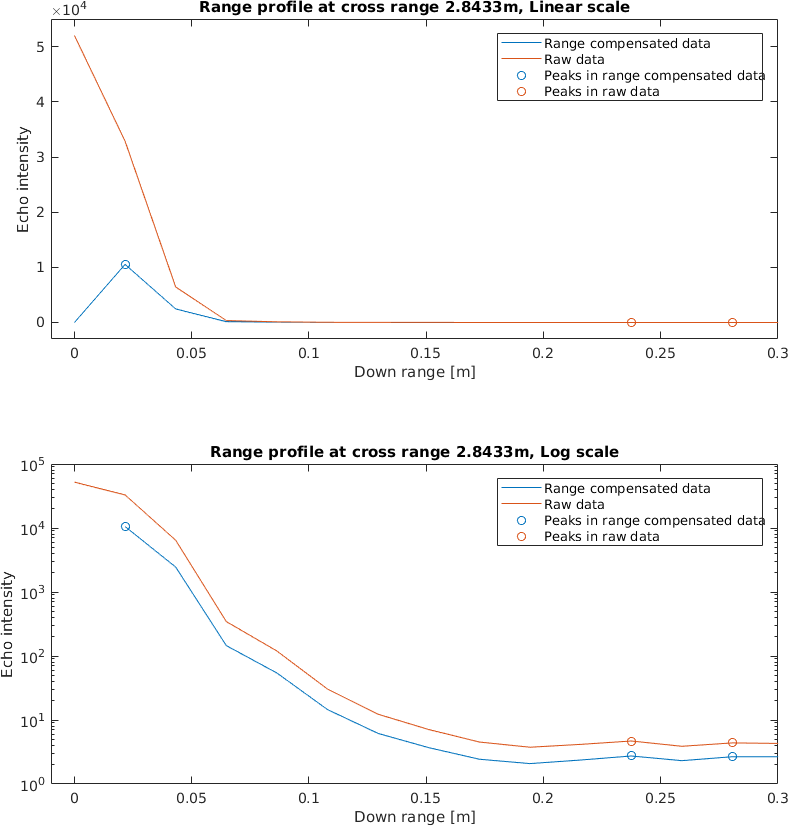
\includegraphics[max height=10cm,max width=10cm]{figures/fig_range_compensation_transmit_spike.png}
    \caption{Attenuating effect of range compensation on transmit peak in range profile}
    \label{fig:fig_range_compensation_transmit_spike}
\end{figure}

Note that the \(0\) value at \(d_{down}=0\) won't be displayed in log
scale.

\subsection{Peaks overlaps at crossing target arcs}\label{peaks-overlaps-at-crossing-target-arcs}

TODO

\subsection{Output}\label{output}

TODO

\subsection{Limitations}\label{limitations-1}

TODO

\subsubsection{Problems with imperfect fit function for subsampling}\label{problems-with-imperfect-fit-function-for-subsampling}

TODO

\subsubsection{Problems with close targets}\label{problems-with-close-targets}

When Doppler speed is measured directly using FMCW, there will be
several Doppler peaks, each representing a different target at the same
range but with individual relative speeds. With the Peak Gradient
Algorithm however, multiple targets at the same range are difficult to
separate. In some cases this is only a temporary problem and is resolved
by the radar moving a little farther so the ranges are separated by more
than the range resolution. Sometimes however some peaks come from
point-like targets that are close together, like a parts of a wall. This
bundle of targets is however not always separated by the same range.
Especially in the case of a wall, the traces of visible points will
cross each other as they slide on the sine arc (see figure). When the
points are close together, only the brightest spots will be seen as
peaks, and the trace of the detected peak matches will describe a
squiggly motion. This causes the estimated Doppler speed to wander
around the common speed. To combat this effect, a higher accumulation
distance can be used during oversampling preprocessing, so the peaks
move together so closely that they actually form a single target.

TODO subcaption with explanation of "simulation"

\begin{figure}[htbp]
    \centering
    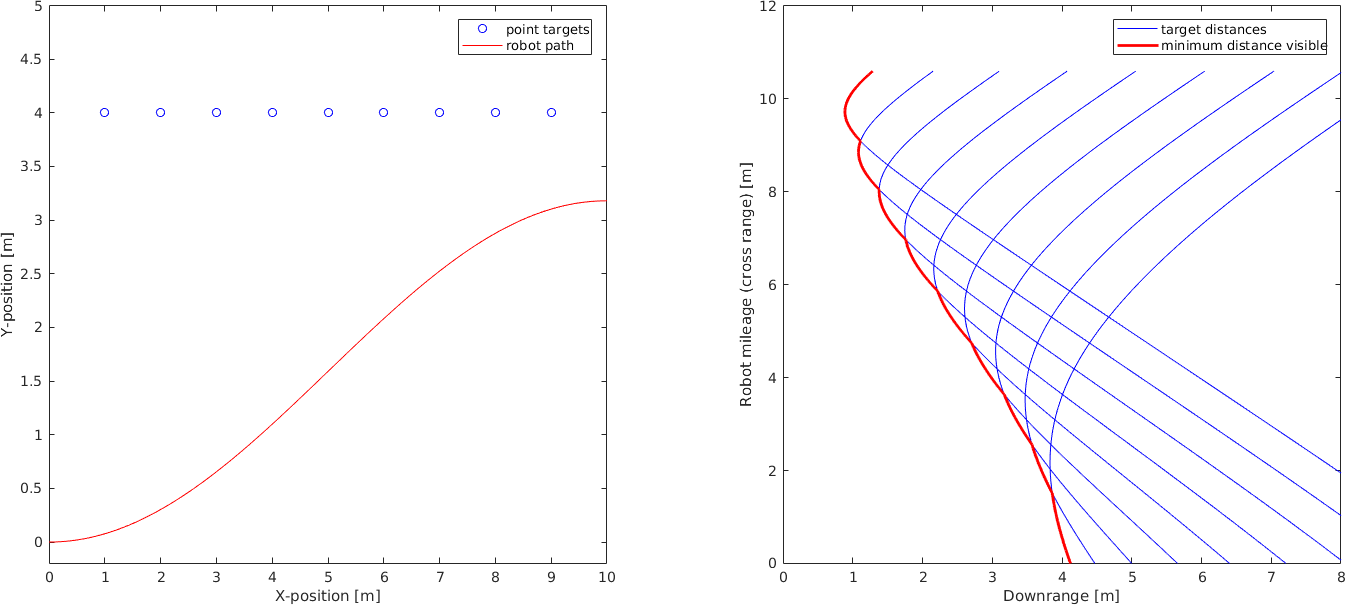
\includegraphics[max height=10cm,max width=10cm]{figures/fig_squiggly_doppler_at_wall}
    \caption{The target echo at the closest range usually has the brightest intensity. This can lead to errors in Doppler speed estimation.}
    \label{fig:fig_squiggly_doppler_at_wall}
\end{figure}

\section{DOA Implementation}\label{doa-implementation}

As described in \cref{direction-of-arrival}, the Direction of Arrival (DOA) angle can be
measured from the phase difference at the receiving antennas of a
multistatic radar.

In the case of RIC60A the antenna separation \(d\) is \(1.16mm\) and
wavelength \(\lambda\) is \(\lambda=\frac{c}{60GHz}=5.0mm\) (with speed
of light \(c\)).

\Cref{fig:fig_range,fig:fig_phase_shift} show the range profile and phase shift of the
``Basement'' scan. The phase shift is very noisy in the regions without
a target peak in the range profile but exhibits steady values following
a gradient over targets.

\begin{figure}[htbp]
    \centering
    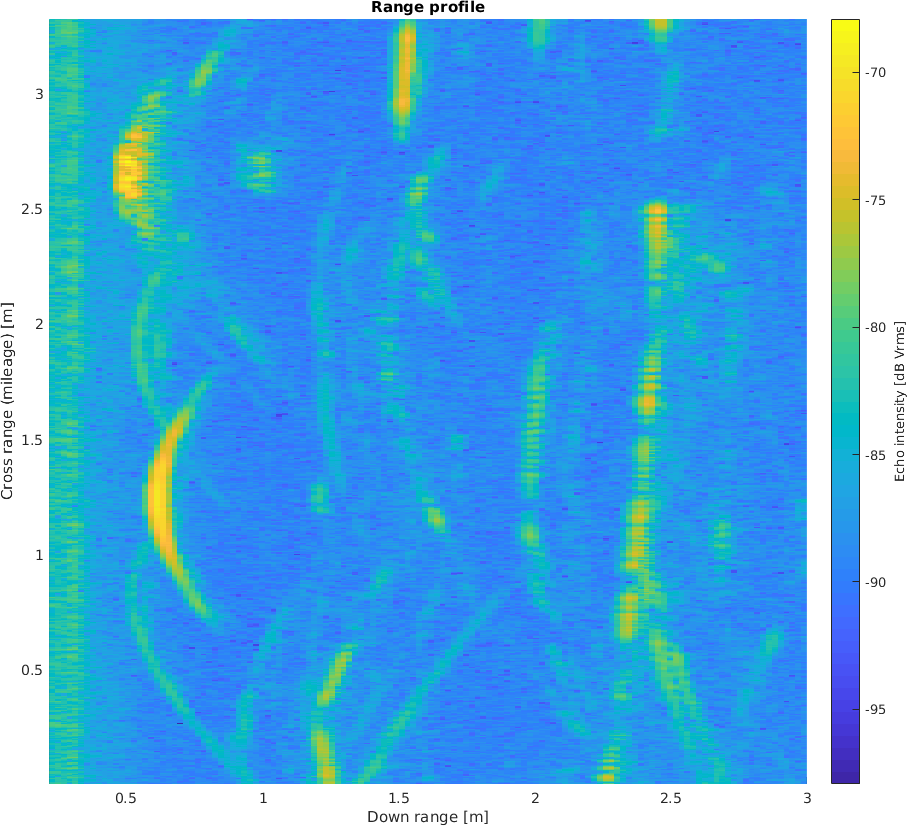
\includegraphics[max height=10cm,max width=10cm]{figures/fig_range}
    \caption{Range profile of Attic scan with color coded echo intensities at cross range over down range}
    \label{fig:fig_range}
\end{figure}

\begin{figure}[htbp]
    \centering
    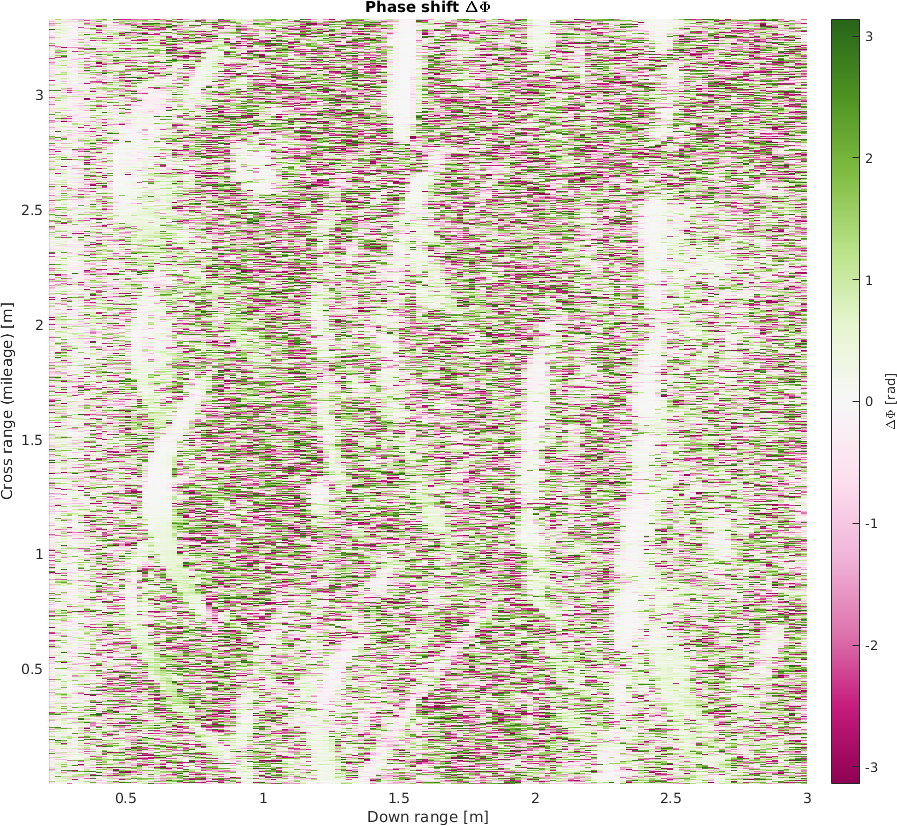
\includegraphics[max height=10cm,max width=10cm]{figures/fig_phase_shift}
    \caption{Phase profile of Attic scan with color coded inter-antenna phase difference at cross range over down range}
    \label{fig:fig_phase_shift}
\end{figure}

Four steps are performed to get a reasonable estimation of direction of
arrival.

\textbf{Peak detection}. In a first step, target peaks in the
range profile are detected. The algorithm records for each peak in each
range scan line its fitted interpolated location, full width at half
maximum, and matching peaks in adjacent lines regarding value and
location.

\textbf{Down range averaging}. In each range scan and at every
detected target peak, the phase shift is averaged over the width of the
respective detected peak. The average is weighted using the Gaussian fit
from subsample peak interpolation.

\textbf{Cross range averaging}. In
every range scan line, each peaks phase shift is averaged over a
configurable accumulation distance in cross range dimension. This is
done by taking the arithmetic mean of all the phase shifts at all
matching peaks (regarding value and down range location) within
accumulation distance in cross range dimension.

\textbf{Cut out}. Noisy
values at non-target peak range bins are masked out.

\textbf{DOA calculation}. In each scan line, each peaks direction of arrival
\(\theta\) is calculated from the smoothed phase shift values, using \cref{eq:doa}.

\Cref{fig:fig_doa} shows the result of these four steps applied on the data of
the ``Basement'' scan. The direction of arrival seems plausible: In this
side-facing scan the robot passed some metal cans. Apparently the radar
sensor was not mounted perfectly orthogonal to the robot's movement
direction (which is not necessary for the reprojection method), but was
slightly off by. This can be seen at the closest points of the target
arcs. At the pericenter the line of sight to a target is orthogonal to
the robot's movement direction, but the DOA value shows to be around 5
to 10 degrees.

\begin{figure}[htbp]
    \centering
    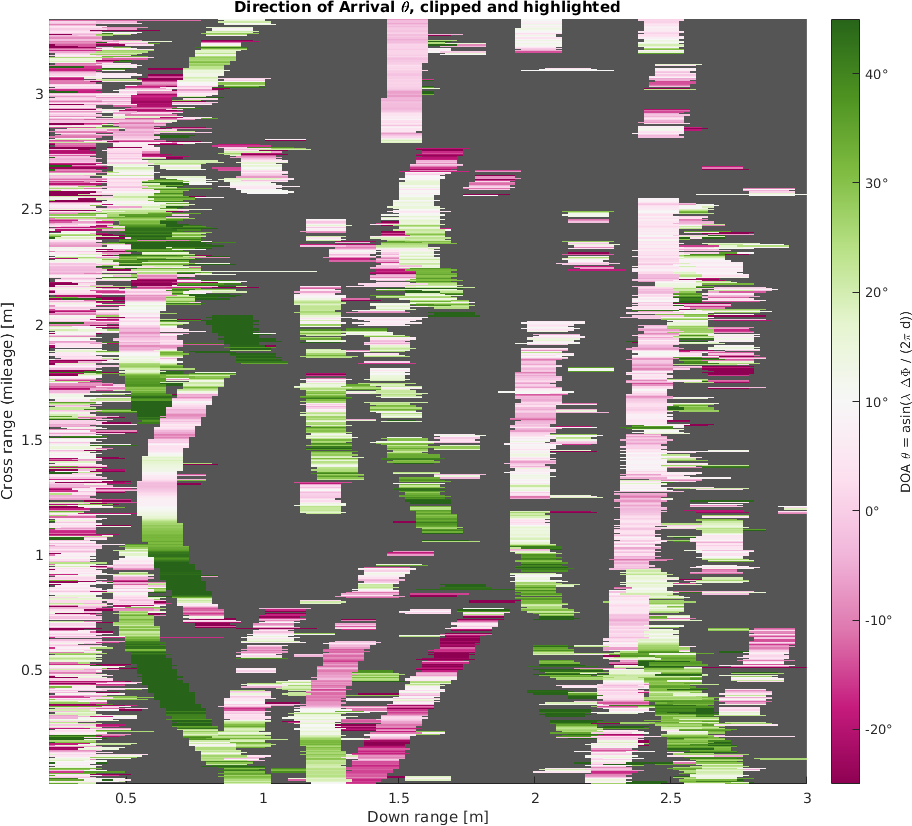
\includegraphics[max height=10cm,max width=10cm]{figures/fig_doa}
    \caption{Direction of arrival estimation for Attic scan}
    \label{fig:fig_doa}
\end{figure}

Note that if the radar sensor is mounted inverted (rotated by 180°), DOA
values have to be multiplied by \(-1\) to keep right and left where they
are.

TODO ric60a doa figure

\section{Reprojection Mapping}\label{reprojection-mapping}

\subsection{Orientation parameters}\label{orientation-parameters}

Before the reprojection can be executed, the physical orientation of the
radar sensor needs to be known to the algorithm. In the implementation,
the two boolean parameters \texttt{forward\_looking} and
\texttt{mount\_inverted} control the behaviour. If the radar's squint
angle and angle sensitivity are such that the field of view reaches both
sides of the robot path, the \texttt{forward\_looking} parameter needs
to be enabled. This enables the processing of DOA data to find the sign
of every target's reprojection angle i.e.~if it is to the left or right
side of the robot's motion path. If the radar is mounted in an
upside-down configuration the squint angle is not affected, but if the
DOA values are processed they need to be mirrored (multiplication with
\(-1\)) because the left and right antennas are switched. Otherwise,
targets will be projected to the wrong side of the robot's path.

\subsection{Projection direction}\label{projection-direction}

The radar reprojection can be executed as forward or backward mapping.
The proof of concept implementation has an optional parameter
\texttt{ProjectionMethod} to switch between forward and backward
mapping.

\subsubsection{Backward mapping}\label{backward-mapping}

If backward mapping is enabled, the reprojection algorithm still
operates range scan line based, but iterates over each pixel in the map.
While this is computationally much more intensive, it allows to add
negative information by reducing the map's value at pixels that are
known to not contain a target because the range scan line does not
feature a peak at that range.

\begin{verbatim}
foreach range_scan_line in range_scan_lines
  foreach pixel in map
    pixel_angle = robot.get_angle_to(pixel)
    distance = robot.get_distance_to(pixel)
    if distance < max_range && pixel_angle in field_of_view_range
      range_bin = range_scan_line.interpolate_at(distance)
      if range_bin.has_peak
        peak_angle = range_bin.peak.doppler.to_angle
        if peak_angle == pixel_angle
          map.at(pixel).add(range_bin.value)
      else
        map.at(pixel).reduce_value
\end{verbatim}

\subsubsection{Forward mapping}\label{forward-mapping}

In forward mapping, the reprojection algorithm iterates over each range
bin in each range scan line. Detected peaks are cut out and reprojected
to a position on the map which is calculated from relative Doppler
speed, range, and robot position. The projection target coordinates
don't usually fall exactly on the map grid points. The implementation
uses sample splitting to distribute a value over the nearest pixels in
this case.

\begin{verbatim}
foreach range_scan_line in range_scan_lines
  foreach peak in range_scan_line
    foreach range_bin in peak
      target_coords = get_coords(robot.position, range_bin.range, peak.doppler)
      weights, neighborhood = split_sample(target_coords)
      map.at(neighborhood).add(weights, range_bin.value)
\end{verbatim}

\subsection{Sample splitting}\label{sample-splitting}

To avoid aliasing when projecting a pixel in the forward projection
direction, the sample is split over the four closest map pixels. The
split is weighted with the distance of the target coordinates to the
closest pixel centers.

If the target coordinate is \(p_{target}=(x_t, y_t)\), then the
horizontal and vertical distributions \(\nu_h\) and \(\nu_v\),
respectively, are \[
\nu_h = \frac{x_t - \lfloor x_t \rfloor}{\lceil x_t \rceil - \lfloor x_t \rfloor} \\
\nu_v = \frac{y_t - \lfloor y_t \rfloor}{\lceil y_t \rceil - \lfloor y_t \rfloor}
\]

The pixel weights \(p_{x,y}\) are then \[
p_{\lfloor x_t \rfloor, \lfloor y_t \rfloor} = \nu_v \nu_h\\
p_{\lfloor x_t \rfloor, \lceil y_t \rceil} = \nu_v (1 - \nu_h)\\
p_{\lceil x_t \rceil, \lfloor y_t \rfloor} =  (1 - \nu_v) \nu_h\\
p_{\lceil x_t \rceil, \lceil y_t \rceil} = (1 - \nu_v) (1 - \nu_h)
\] , such that \[
\sum\limits_{
x \in \{\lceil x_t \rceil, \lfloor x_t \rfloor\}\\
y \in \{\lceil y_t \rceil, \lfloor y_t \rfloor\}
} p_{x,y} = 1
\]

In the special case where $y\_t = \lceil y\_t \rceil = \lfloor y\_t\rfloor$ there are only two instead of the four neighboring pixels. Their weights \(p_{x,y}\) are \[
p_{\lfloor x_t \rfloor, y_t} = \nu_h\\
p_{\lceil x_t \rceil, y_t} = (1 - \nu_h)
\] The same applies when $x\_t = \lceil x\_t \rceil = \lfloor x\_t\rfloor$: \[
p_{x_t, \lfloor y_t \rfloor} = \nu_v\\
p_{x_t, \lceil y_t \rceil} = (1 - \nu_v)
\] And lastly, if
(\(y_t = \lceil y_t \rceil = \lfloor y_t \rfloor ) \land (x_t = \lceil x_t \rceil = \lfloor x_t \rfloor )\),
then \(p_{x_t, y_t} = 1\)

\begin{figure}[htbp]
    \centering
    \def\svgwidth{10cm}
    \input{gfx/diagrams/sample_splitting.pdf_tex}
    \caption{Illustration of a pixel value (white circle) being distributed over the four nearest grid neighbors. The shade of the neighbor's area indicates the individual distrution weight.}
    \label{fig:Sample_splitting}
\end{figure}

\subsection{Range compensation}\label{range-compensation}

As evident from the classical radar \cref{eq:radarclassical}, echo intensity decreases with
the fourth power of distance. This has the effect that reprojected
targets appear brighter when they are mapped from close distance; but
most importantly, when targets are detected from a far distance, mapped
intensities are decreased due to the map's averaging.

This attenuation can be compensated with a range-based compensation
factor \(f_r\) with \[f_r(d_{down}) = {
\left(
c_a + (
\frac{{d_{down}}{c_b}}
+ c_c)^{-4}
\right) ^ {-1}
}\]



\Cref{fig:fig_range_compensation} shows the range profile of the ``Torture Chamber'' scan
both as oversampled raw values (top subplot) and with range compensation
enabled (bottom subplot). The middle subplot details the range scan line
at one cross range highlighted by the red lines. Inspecting this detail
graph reveals that both target peaks and noise floor are lowered in the
near range, while the noise floor stays constant in the far range. This
helps to keep a target's intensity at at least similar values over all
ranges in the map.

TODO subfigures, adjust refs
\begin{figure}[htbp]
    \centering
    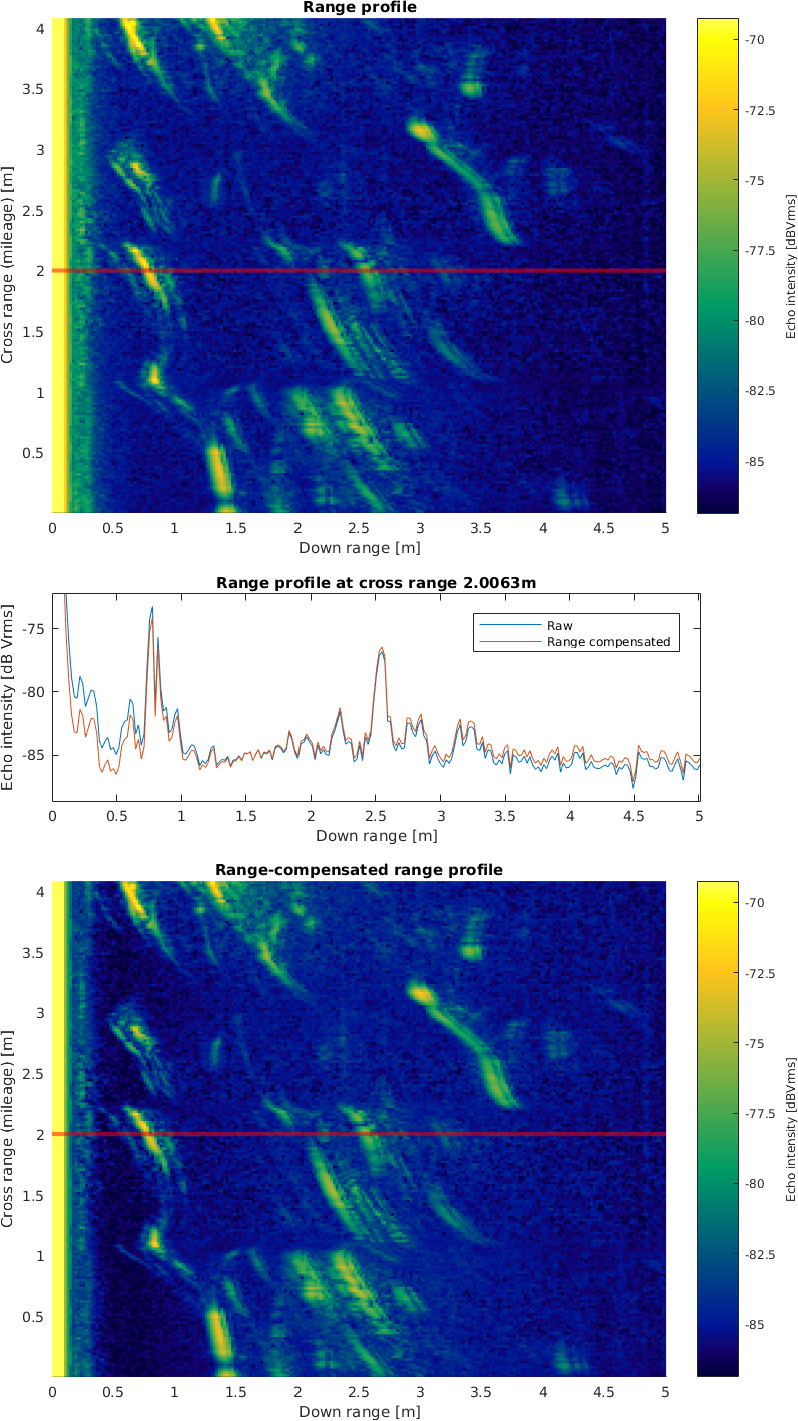
\includegraphics[max height=10cm,max width=10cm]{figures/fig_range_compensation}
    \caption{Range compensation}
    \label{fig:fig_range_compensation}
\end{figure}

\subsection{Angle sensitivity compensation}\label{angle-sensitivity-compensation}

The intensity of a target peak depends on its angle with respect to the
antenna. The angle is unknown before the Doppler speed is estimated, so
the knowledge about echo attenuation caused by antenna angle sensitivity
can not be used to improve peak detection. But the echo intensity
influences how a target is represented on the reprojection map. Since
the map averages all reprojections to any given point a low intensity
echo will reduce the visibility of a target on the map. This can however
be compensated by multiplying detected target peak heights with a factor
that is based on the angle the target is believed to be seen under.

The angle compensation factor curve was found by experiment. A strong
point target (a retroreflector) was placed at a known range away from
the robot. The robot was then made to rotate around itself, such that
the target comes into view and leaves again. Meanwhile, the radar scans,
together with robot odometry were recorded.

The radar was not mounted over the center of rotation of the robot. This
way, the radar did describe a circular path whose mileage can be
calculated. The angle compensation measurement can hence be visualized
in figure \cref{fig:fig_range_compensation} in the usual range profile with echo intensities over
cross versus down range. The range of the retroreflector varies with
twice the distance of the radar to the robot's rotation center, but only
the orientation is interesting - the range can just be summed up over
the range bins the target is visible in (in this case,
\(0.45m - 0.85m\)).

In figure \cref{fig:fig_range_compensation}, the same range scan lines are sorted by robot
orientation during the scan. After the explained summing in down range
dimension the intensity (absolute value of complex signal) data of both
antennas is binned separately over 60 orientations from \(-\pi\) to
\(\pi\).

The manufacturer later provided angle sensitivity measurements of the
IC's batch (see figure TODO). The measurements show that the
experimental approach produced valid results.

The compensation factor \(f_a\) for each angle is finally composed using
the formula

\[m = \max \left( \max (s_{Rx1}), \max (s_{Rx2}) \right)\] \[
f_a = \frac{1}{2}
  \left(
    \frac{m}{ s_{Rx1} } +
    \frac{m}{ s_{Rx2} }
  \right)
\]

Multiplicating a peak which is to be reprojected at angle \(\alpha\)
with angle compensation factor \(f_a(\alpha)\) results in a peak height
that is independent of observation angle.

\begin{figure}[htbp]
    \centering
    \begin{subfigure}{\textwidth}
        \centering
        \def\svgscale{0.8} \small
        \input{gfx/fig_svg/angle_compensation_1.pdf_tex}
        \caption{Range profile, as recorded}
        \bigskip
    \end{subfigure}
    \begin{subfigure}{\textwidth}
        \centering
        \def\svgscale{0.8} \small
        \input{gfx/fig_svg/angle_compensation_2.pdf_tex}
        \caption{Range profile, sorted by robot orientation}
        \bigskip
    \end{subfigure}
    \begin{subfigure}{\textwidth}
        \centering
        \def\svgscale{0.8} \small
        \input{gfx/fig_svg/angle_compensation_3.pdf_tex}
        \caption{Echo intensity between 0.4m and 0.8m down range, and compensation factor normalizing intensity}
        \bigskip
    \end{subfigure}
    \caption{Angle compensation factor}
    \label{fig:fig_angle_compensation}
\end{figure}

\subsection{Angle compensation window}\label{angle-compensation-window}

Detected peaks are not in a single range bin, but form a curve over
several range bins. Multiplicating each of these range bin's values with
the same \(f_a\) does work, but leaves hard edges. It is better to
multiplicate the peak with a window function with height \(f_a\). The
implementation the window \(w\):
\[
w(x,f_a) = 1 + (f_a - 1) ~e ^ { -\frac{ \left( {x - p_x} \right) ^ 2 } {p_w} }
\] where \(p_x\) is the peaks subsample-interpolated peak location in
down range space and
\[
p_w = \cfrac{
\left( \frac{fwhm}{4}  \right) ^2
}{
4 ln(2)}
\]
is
the peaks width, where \(fwhm\) is the full width at half maximum as
found by the subsample-interpolated peak fit.

\Cref{fig:fig_angle_compensation_comparison} show a glass wall in the ``Racetrack'' scan. In \cref{fig:fig_angle_compensation_comparison_1}, only range compensation is applied. In \cref{fig:fig_angle_compensation_comparison_2},
angle compensation is switched on. In \cref{fig:fig_angle_compensation_comparison_3}, both angle
compensation and angle compensation windowing are switched on. The
figure shows how angle compensation helps to keep the echo intensity of
a mapped object at the same level, regardless of the angle at which it
is seen by the radar.

TODO replace vector heatmap with bitmap
\begin{figure}[htbp]
    \centering
    \begin{subfigure}{\textwidth}
        \centering
        \def\svgscale{0.8} \small
        \input{gfx/fig_svg/angle_compensation_comparison_1.pdf_tex}
        \caption{Reprojected energy, without angle compensation}
        \label{fig:fig_angle_compensation_comparison_1}
        \bigskip
    \end{subfigure}
    \begin{subfigure}{\textwidth}
        \centering
        \def\svgscale{0.8} \small
        \input{gfx/fig_svg/angle_compensation_comparison_2.pdf_tex}
        \caption{Reprojected energy, with angle compensation}
        \label{fig:fig_angle_compensation_comparison_2}
        \bigskip
    \end{subfigure}
    \begin{subfigure}{\textwidth}
        \centering
        \def\svgscale{0.8} \small
        \input{gfx/fig_svg/angle_compensation_comparison_3.pdf_tex}
        \caption{Reprojected energy, with windowed angle compensation}
        \label{fig:fig_angle_compensation_comparison_3}
        \bigskip
    \end{subfigure}
    \caption{Effect of angle compensation and windowed angle compensation}
    \label{fig:fig_angle_compensation_comparison}
\end{figure}


\subsection{World map resolution}\label{world-map-resolution}

TODO

\chapter{Results and Evaluation}\label{results-and-evaluation}

\section{Evaluation}\label{evaluation}

Before the results of the presented proof-of-concept implementation are listed it needs to be clear what dimensions are important so that a distinction between good and bad results can be made.

A good reprojection map has several qualities that make it usable as an obstacle gridmap. First, it needs to be \textbf{timely}. That means that the time between the appearance of an object in the robot's path and it being mapped in an obstacle map needs to be small enough that the robot can still avoid collisions. The \textbf{false alarm rate}, representing false positive detections, needs to be low enough to not negatively influence the robot's navigation behaviour by making it circumnavigate phantom obstacles. Vice versa, the \textbf{missed target rate}, or false negative detection needs to be low, or the radar sensor will not bring an advantage over conventional obstacle sensors. The resulting map of course also needs to be \textbf{spatially correct}. This means that a detected obstacle is mapped at its true location. Otherwise, phantom obstacles or incorrectly sized obstacles will degrade map quality. The map becomes more useful if it contains \textbf{diverse types of obstacles}, and not just one class of objects, like walls. On the other hand, it should not contain \textbf{irrelevant information}, for example wall temperature is not interesting for obstacle detection. Lastly, only if the map is \textbf{comparable to other sensors} informed comparison can take place. For example, a glass wall is easily visible to the human eye, so their position in the radar reprojection map can be verified. But metal struts in walls, which, while not presenting an obstacle to the robot (vacuum robots usually are not designed to breach walls), could be useful landmarks for later slam applications, are not visible in other maps. Hence the quality of metal strut mapping can not be asserted, but only assumed based on human knowledge of where a wall's metal struts might be.

There are some classes of targets that are particularly interesting in the evaluation of results. The first one is stacks of \textbf{metal cans}, because they appear in many of the scans. This is a kind of artificial obstacle that was designed to have a high probability of visibility in both radar scans (the curved metal surface is very reflective from every direction) and lidar scans (the can towers are high enough to cross the laser beam, and wide enough to not be missed even in some distance). Another easy target are \textbf{walls}. They are easy to see in the lidar scan, and detections in the radar reprojection map can be easily compared. A special case of walls are \textbf{glass walls} or windows. They present an impenetrable obstacle in a robots path, but almost always, neither a laser scanner nor a vision sensor can detect them (see \cref{fig:rgbd_glasswall2}). Another real world obstacle that escapes lidar scans are \textbf{office chair legs}. While the pillar is visible with laser (green dot in \cref{fig:lidar_rgbd2}), the horizontally stretching legs and rollers are usually too low to be detected. In the same category of low profile obstacles are \textbf{cables} lying on the floor. A vacuum robot can easily entangle in them and get stuck. Lastly, it would be interesting to see negative obstacles including \textbf{cliffs} and dips. Today, robots need an extra set of sensors (usually IR distance sensors at the front of the robot, aiming at the floor) to detect this kind of obstacle very reliably.

\begin{figure}
  \begin{subfigure}[t]{.485\textwidth}
      \centering
      \def\svgwidth{\linewidth}
      \input{gfx/screenshots/rgbd_glasswall.pdf_tex}
      \caption{RGBD camera can not detect glass surface.}
      \label{fig:rgbd_glasswall2}
  \end{subfigure}%
  \hfill%
  \begin{subfigure}[t]{.485\textwidth}
      \centering
      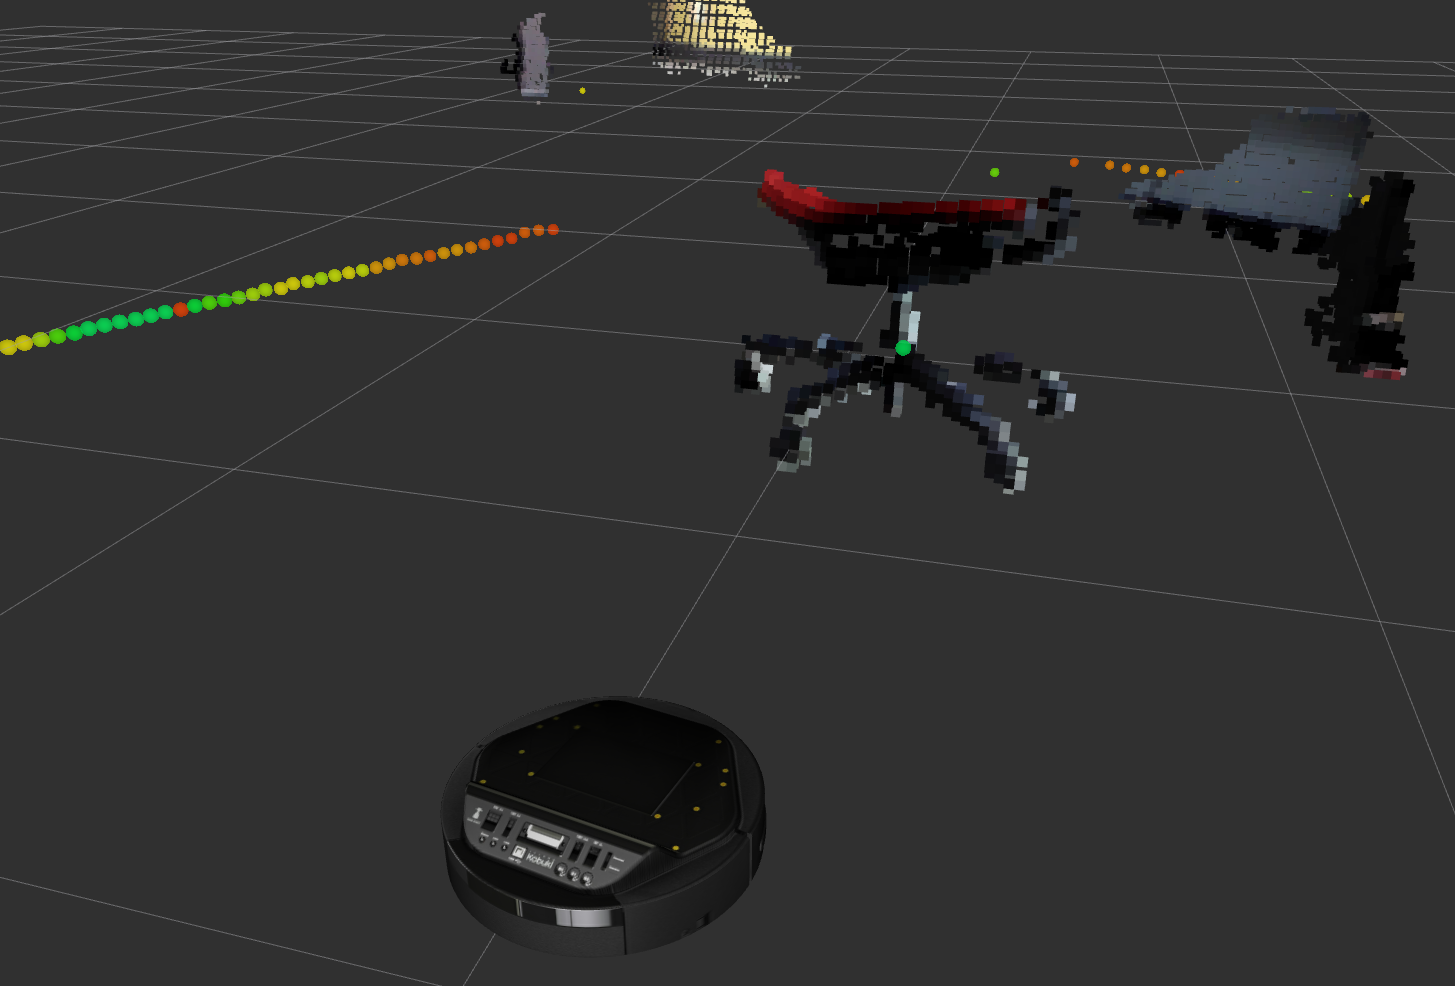
\includegraphics[max width=\textwidth]{gfx/screenshots/chair_laser_vs_rgbd}
      \caption{Laser fails to detect horizontal chair legs.}
      \label{fig:lidar_rgbd2}
  \end{subfigure}%
  \caption{Screenshots showing traditional sensor shortcomings.}
\end{figure}


\section{Results}\label{results}

During development of the reprojection method, over 30 scans were taken. The environment for the scans is the BSH office in the Bosch Research and Technology Center in Palo Alto, which is fairly representative of a typical office environment. It has carpet floors, desks, office chairs, walls, corridors, and even glass walls.

The scans of this environment are assigned code names in alphabetical order for easy referencing. \Cref{tab:params} shows the parameters with which each of the scans was taken: Sweep time, sensor orientation (\textbf{H}orizontal / \textbf{V}ertical / \textbf{H}orizontal \textbf{I}nverted beam fan), squint angle (center of sensor's FOV, so \ang{90} is sideways-looking and \ang{0} is forward-looking), mounted horn antenna extension (which narrows the beam shape), availability of \texttt{/map} rosmessages with lidar slam information, and finally availability of \texttt{/tf} rosmessages which carry the slam-based odometry drift correction.

The scans are presented through the following plot types. An exemplary result is shown in \cref{fig:nirvana} and more result plots can be found in \cref{scans}

\subparagraph{Input Energy}
This plot (e.g. \cref{fig:resinput}) visualizes the preprocessed (i.e. oversampled, range and transmit crosstalk compensated) input energy of a scan. To understand the graph, it helps to first think of it as the stacked range profile of a range sensor that looks in a \ang{90} angle to the right of the robot. The x-axis represents down-range (in \si{m}), which is the range axis in the 1D range profile as extracted from the FMCW beat frequency (see \cref{fig:rawbeat_f} for an example). Each range profile line's echo intensity (shown on the y-axis in \cref{fig:rawbeat_f}) is visualized in a logarithmic \texttt{hcparula}\footnote{\texttt{hcparula} is a monotonic, linear-grayscale intensity colormap with enhanced contrast. It is available at \url{https://www.mathworks.com/matlabcentral/fileexchange/61768}} color scale. The unit is \si{dB Vrms}. These range lines are stacked over the Y-axis direction, which is the cross-range dimension. This dimension shows how far the radar sensor has traveled from the scan's origin (i.e. mileage, in \si{m}). If the radar was moved at a constant velocity, it can be thought of as the time axis, however denoting and processing it as mileage has the benefit of radar velocity independence. Note that this plot does not show any information on where (at which angle) a target is, but only at what distance it is. Target peaks appear and disappear over the course of the y-axis, because they enter or leave the radar antenna's field of view.

\subparagraph{Doppler estimation}
To calculate reprojection angles, a target's Doppler speed must be estimated. This graph (e.g. \cref{fig:resdoppler}) shows the estimation from the peak gradient algorithm: Every detected peak has a certain speed associated with it. This speed is plotted as color over the FWHM around the peak's location in down-range/cross-range space. The color follows a symmetric linear pink/white/green color scale\footnote{Specifically, \texttt{PiYG} via the \texttt{cbrewer} function, which is available at \url{https://www.mathworks.com/matlabcentral/fileexchange/34087}}. The estimated Doppler speed is not shown in its smoothed version, which is averaged over cross range as described in \cref{raw-data-smoothing} and peak FWHM as described in \cref{peaks-overlaps-at-crossing-target-arcs}. The background of the graph is dark grey to make sure the white middle of the color scale is visible, as well as to help highlight where Doppler peaks were actually detected.

\subparagraph{DOA estimation}
The third input graph (e.g. \cref{fig:resdoa}) shows DOA data as estimated in \cref{doa-implementation}, which in the current implementation is solely used to resolve the left-right reprojection angle ambiguity in the forward-looking geometry (see \cref{geometry-for-the-general-case}). The (darkened) graph background visualizes the phase difference of the oversampled complex analytic input signal of both receiving radar antennas. Similar to the Doppler graph, DOA information over detected peaks is smoothed over cross-range and each peak's FWHM. The color is the same symmetric pink/white/green as the Doppler plot. The color scale is from $-\pi/3$ to $\pi/3$ radian; values above or below are clipped (but this happens only for the noisy background signal).

\subparagraph{Reprojection map}
This is the main output of the reprojection mapping implementation, as described in \cref{reprojection-mapping}. The graph (e.g. \cref{fig:resrepro}) shows a top-view 2D map, with the origin (0,0) at the scan starting point. Axes are in \si{m}. The color scale is again \texttt{hcparula}, with echo intensities in \si{dBVrms}. The red line shows the radar motion path.

\subparagraph{Reprojection map overlay}
If the \texttt{/map} is available for a scan, this graph (e.g. \cref{fig:resmap}) shows the reprojection map overlaid over the lidar occupancy gridmap as described in \cref{output}. The lidar map has a grayscale colormap, where black means occupied, white means clear, and anything in between shows occupancy probability. Uncharted, unknown values are a ``tasteful blueish greenish grayish color''\footnote{Legal \texttt{-1} value from \url{http://docs.ros.org/jade/api/rviz/html/c++/map\_\_display\_8cpp\_source.html\#l00212}}. The red path is again the radar motion path.


\begin{table}[htb]
  \caption{Scan parameters}
  \label{tab:params}
  \rowcolors{1}{ColorAlternatedRow}{}
    \begin{tabularx}{\textwidth}{%
      >{\setlength{\hsize}{.31\hsize}\raggedright\arraybackslash}X%
      >{\setlength{\hsize}{.15\hsize}\raggedright\arraybackslash}X%
      >{\setlength{\hsize}{.12\hsize}\raggedright\arraybackslash}X%
      >{\setlength{\hsize}{.12\hsize}\raggedright\arraybackslash}X%
      >{\setlength{\hsize}{.10\hsize}\centering\arraybackslash}X%
      >{\setlength{\hsize}{.10\hsize}\centering\arraybackslash}X%
      >{\setlength{\hsize}{.10\hsize}\centering\arraybackslash}X%
    }
    \hiderowcolors
    \toprule
Name & Sweep & Orient. & Squint & Horn & Map & TF \\
    \midrule
    \endhead

    \bottomrule
    \endfoot
    \showrowcolors
    %
 Attic & \SI{5.0}{ms} & H & \ang{90} & \cmark & \xmark & \xmark \\
 Basement & \SI{5.0}{ms} & H & \ang{90} & \cmark & \xmark & \xmark \\
 Cafeteria & \SI{5.0}{ms} & H & \ang{90} & \cmark & \xmark & \xmark \\
 Dungeon & \SI{5.0}{ms} & V & \ang{20} & \cmark & \xmark & \xmark \\
 Entryway & \SI{5.0}{ms} & V & \ang{20} & \cmark & \xmark & \xmark \\
 Fallout Shelter & \SI{5.0}{ms} & V & \ang{20} & \cmark & \xmark & \xmark \\
 Garden & \SI{5.0}{ms} & V & \ang{20} & \cmark & \xmark & \xmark \\
 Home Cinema & \SI{5.0}{ms} & V & \ang{20} & \cmark & \xmark & \xmark \\
 Indoor Swimming Pool & \SI{5.0}{ms} & V & \ang{20} & \cmark & \xmark & \xmark \\
 Jail Cell & \SI{5.0}{ms} & H & \ang{20} & \cmark & \xmark & \xmark \\
 Kitchen & \SI{5.0}{ms} & H & \ang{20} & \xmark & \xmark & \xmark \\
 Lobby & \SI{5.0}{ms} & H/I & \ang{0} & \xmark & \xmark & \xmark \\
 Mancave & \SI{5.0}{ms} & H/I & \ang{0} & \xmark & \xmark & \xmark \\
 Nirvana & \SI{5.0}{ms} & H/I & \ang{0} & \xmark & \cmark & \xmark \\
 Orbit & \SI{5.0}{ms} & H/I & \ang{0} & \xmark & \cmark & \xmark \\
 Public Restroom & \SI{5.0}{ms} & H/I & \ang{0} & \xmark & \cmark & \cmark \\
 Queue & \SI{20}{ms} & H/I & \ang{0} & \xmark & \cmark & \cmark \\
 Racetrack & \SI{2.0}{ms} & H/I & \ang{0} & \xmark & \cmark & \cmark \\
 Sauna & \SI{2.5}{ms} & H/I & \ang{0} & \xmark & \cmark & \cmark \\
 Torture Chamber & \SI{2.5}{ms} & H/I & \ang{45} & \xmark & \cmark & \cmark \\
 Underground & \SI{2.5}{ms} & H/I & \ang{45} & \xmark & \cmark & \cmark \\
 Virtual Reality & \SI{2.5}{ms} & H/I & \ang{45} & \xmark & \cmark & \cmark \\
 Washroom & \SI{2.5}{ms} & V & \ang{45} & \xmark & \cmark & \cmark \\
 Xray-Room & \SI{2.5}{ms} & V & \ang{0} & \xmark & \cmark & \cmark \\
 Y Is There A Cable On The Floor & \SI{5.0}{ms} & V & \ang{0} & \xmark & \cmark & \cmark \\
%  Z & & & & & & \\
    \end{tabularx}
\end{table}

\begin{figure}[htbp]
    \centering
    \begin{subfigure}[t]{0.32\linewidth}
        \centering
        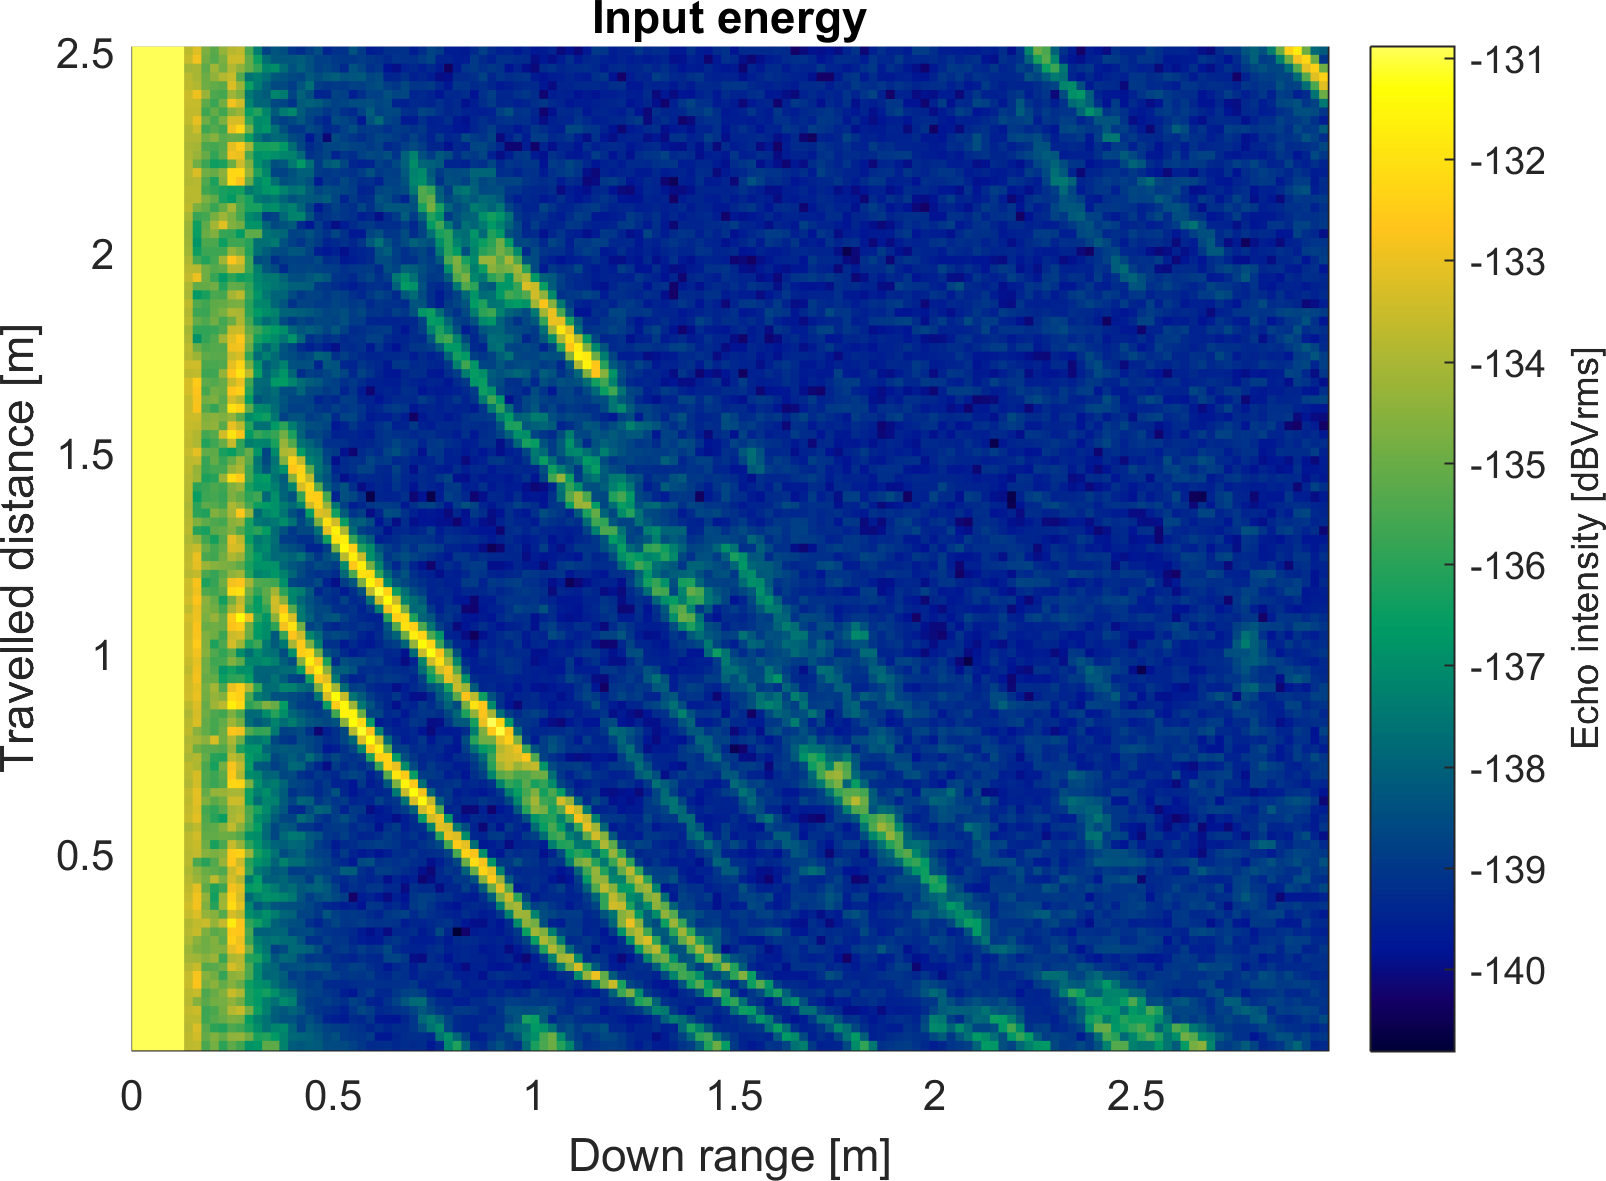
\includegraphics[width=\linewidth]{gfx/results/nirvana_input.png}
        \caption{\small Input energy} \label{fig:resinput}
    \end{subfigure}%
    \hfill%
    \begin{subfigure}[t]{0.32\linewidth}
        \centering
        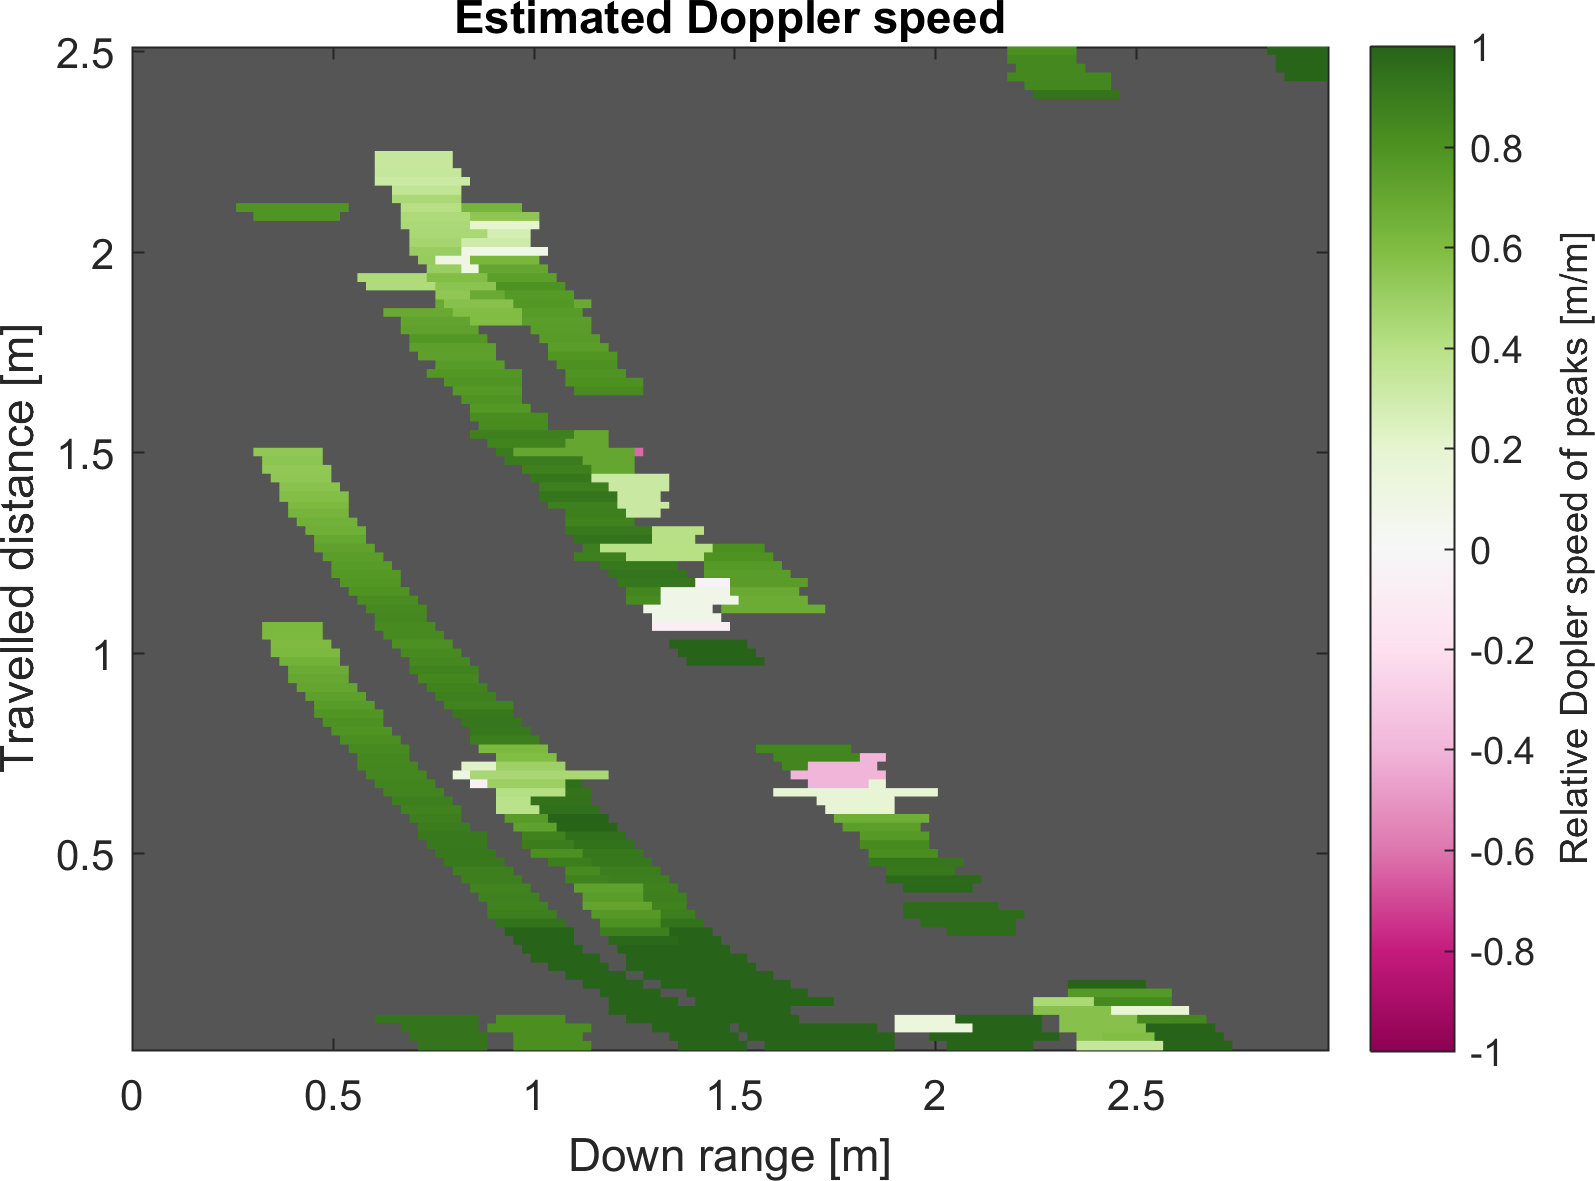
\includegraphics[width=\linewidth]{gfx/results/nirvana_doppler.png}
        \caption{\small Doppler estimation} \label{fig:resdoppler}
    \end{subfigure}%
    \hfill%
    \begin{subfigure}[t]{0.32\linewidth}
        \centering
        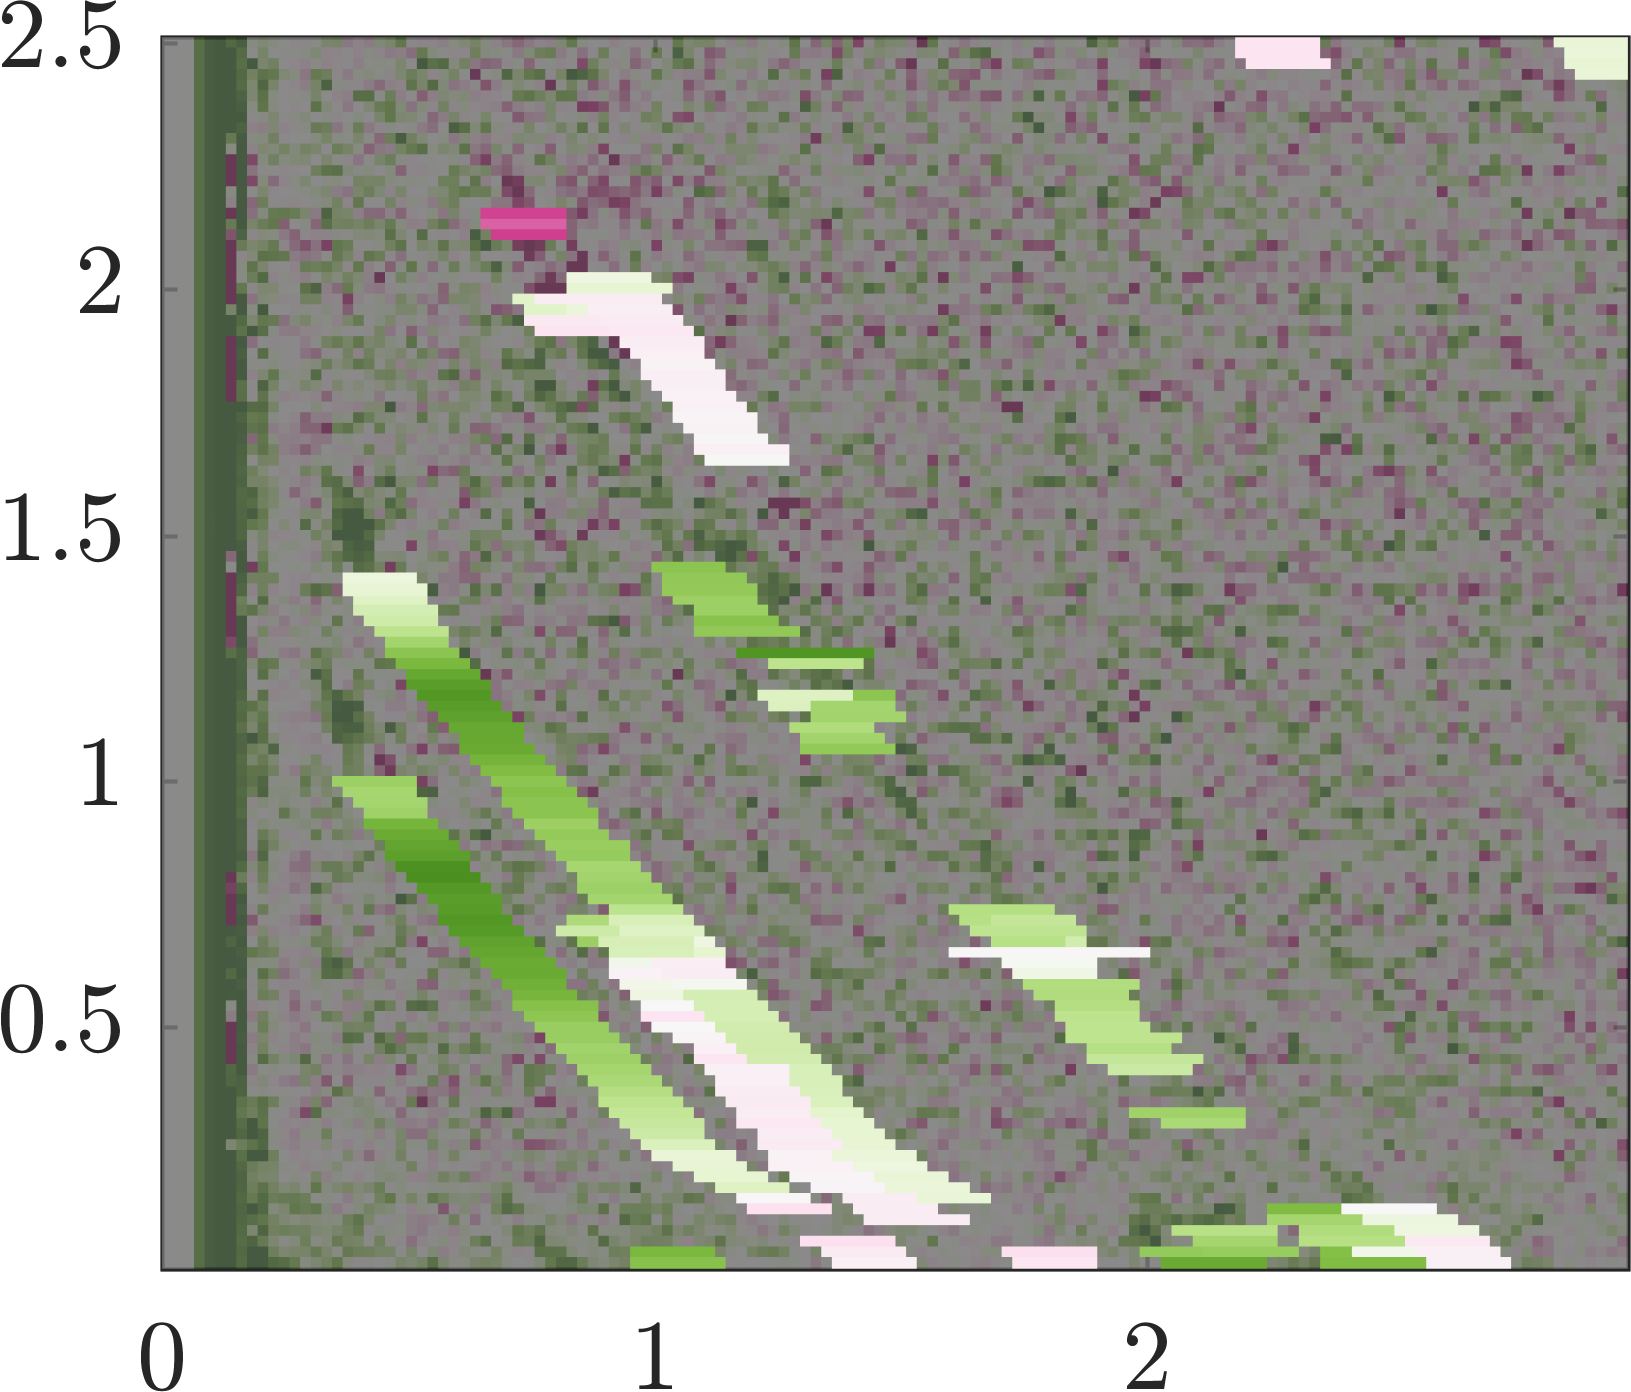
\includegraphics[width=\linewidth]{gfx/results/nirvana_doa.png}
        \caption{\small Direction of Arrival} \label{fig:resdoa}
    \end{subfigure}\\
    \begin{subfigure}[t]{0.475\textwidth}
        \centering
        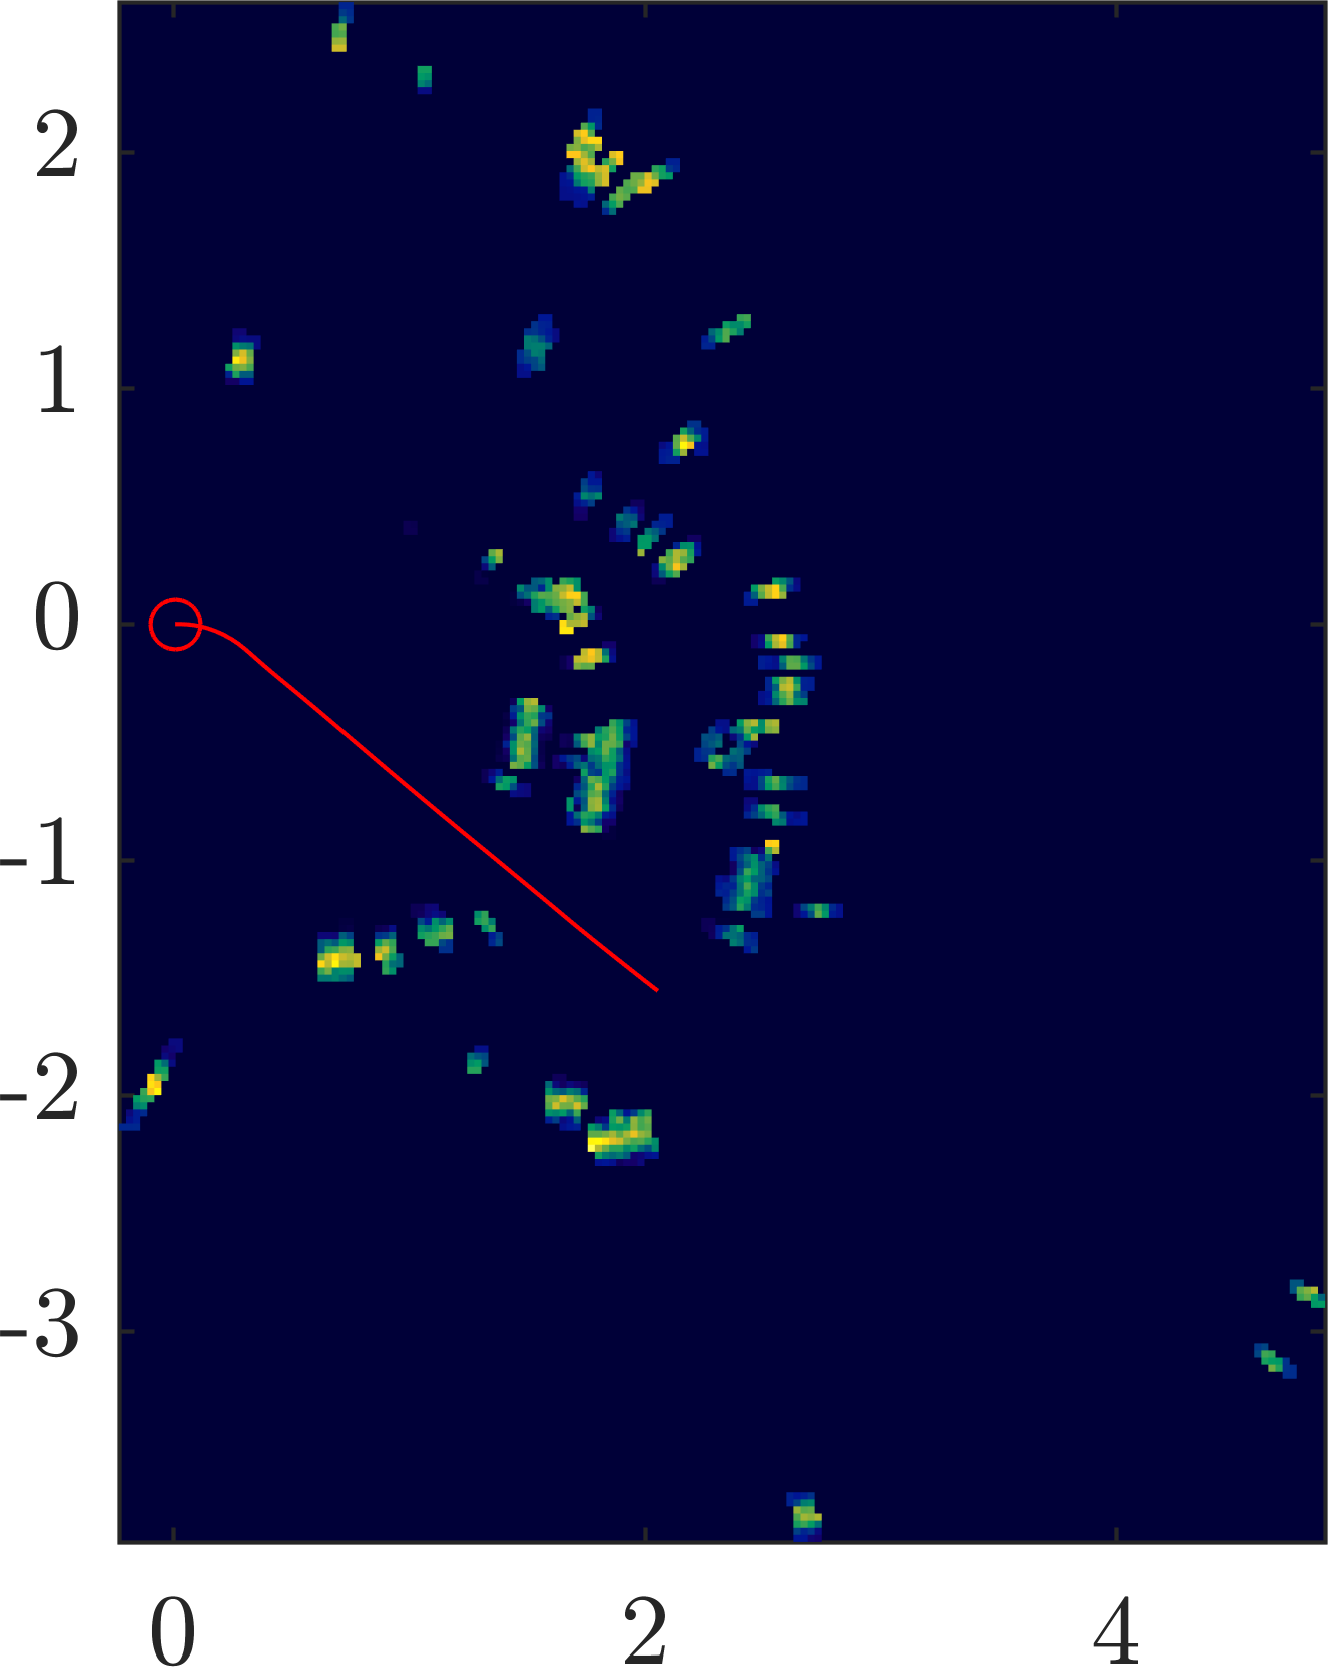
\includegraphics[max width=\linewidth, max height=\linewidth]{gfx/results/nirvana_reprojection.png}
        \caption{\small Reprojection Map} \label{fig:resrepro}
    \end{subfigure}%
    \hfill%
    \begin{subfigure}[t]{0.475\textwidth}
        \centering
        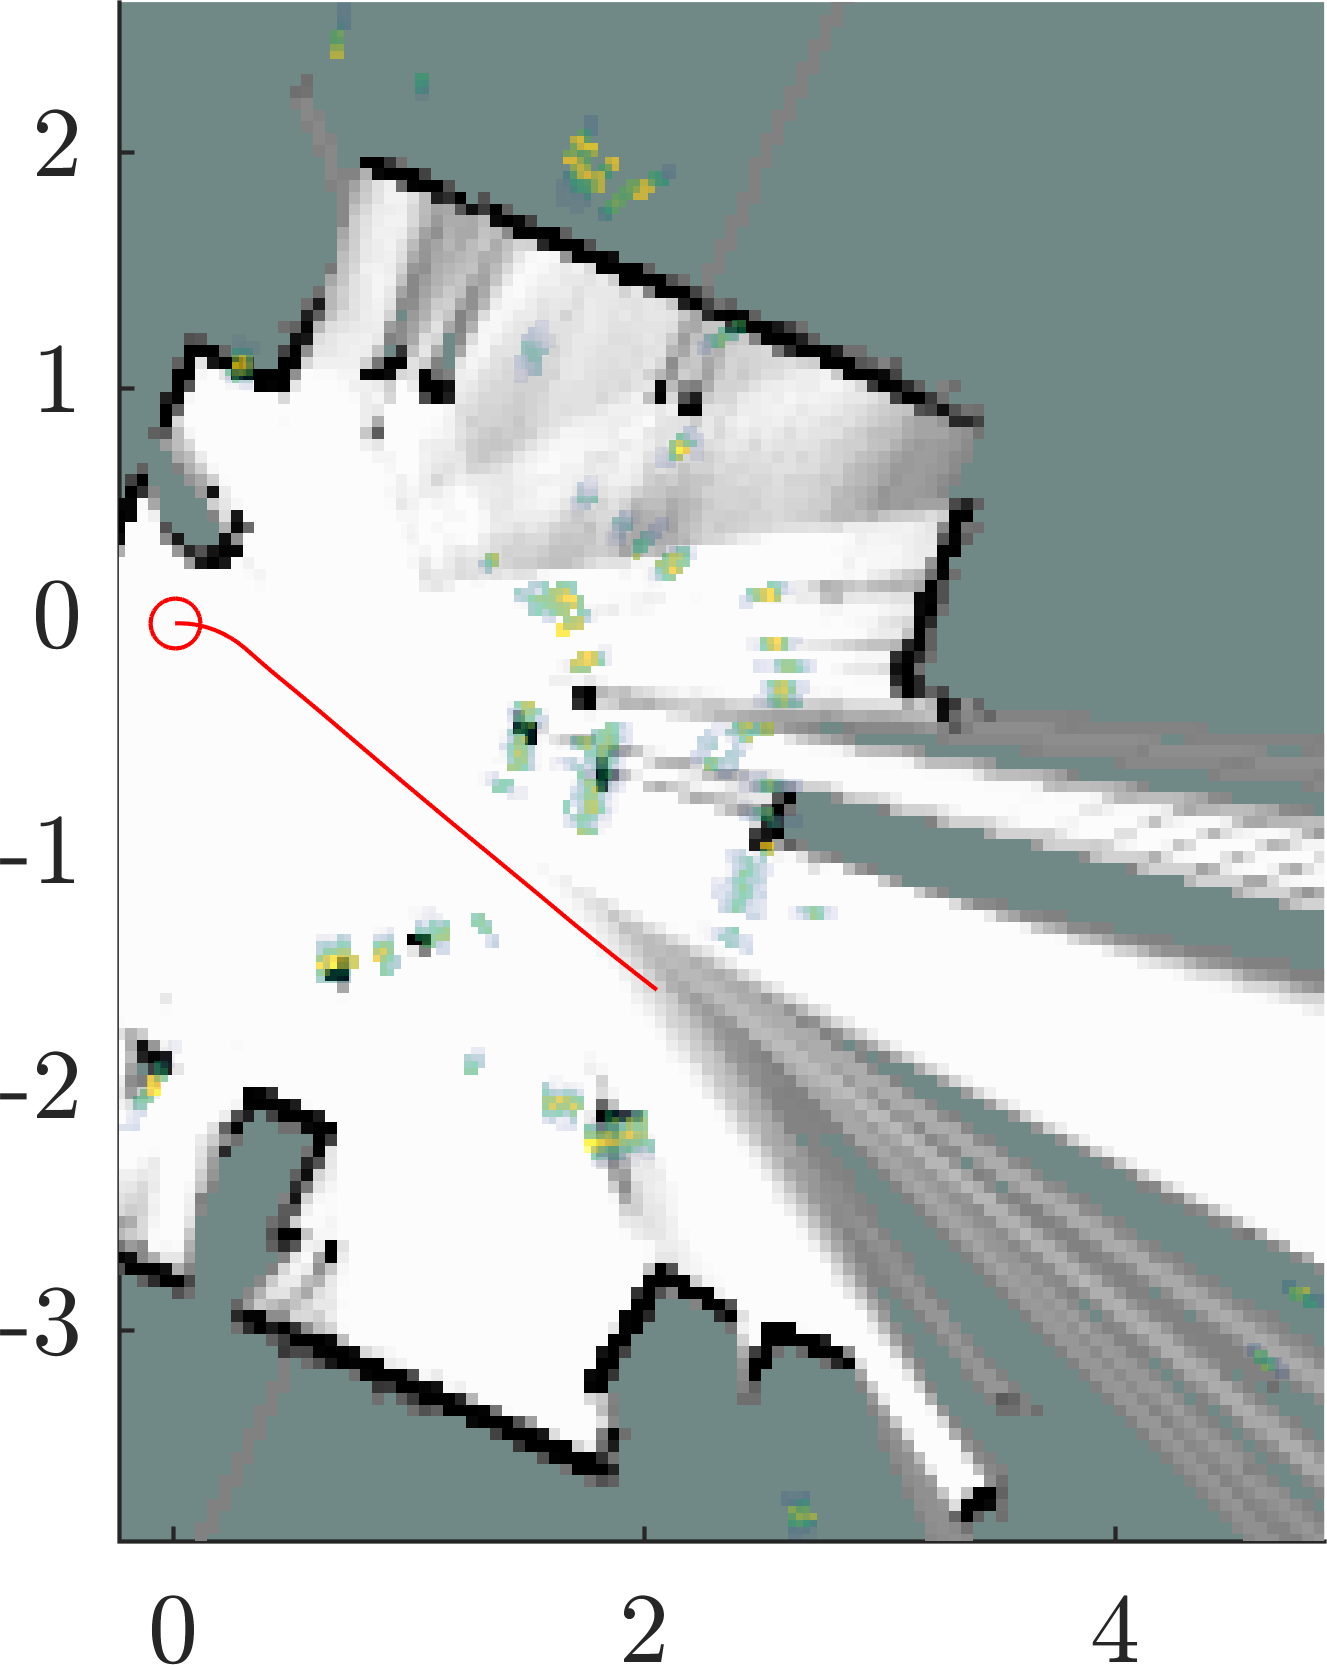
\includegraphics[max width=\linewidth, max height=\linewidth]{gfx/results/nirvana_map.png}
        \caption{\small Reprojection Map} \label{fig:resmap}
    \end{subfigure}%
    \caption{Nirvana scan} \label{fig:nirvana}
\end{figure}

\chapter{Discussion and Comparison}\label{discussion-and-comparison}

TODO: intro to discussion topics. was the initial hypothesis validated?

\section{Discussion}

\subsection{Reflection directionality}\label{reflection-directionality}

Many objects only become visible when their surface is oriented
perpendicularly to the incident radar waves, so that enough scattered EM
energy makes its way back to the sensor. This is very visible in the
Underground scan, where a glass wall is detected as the robot passes it,
but not while the robot sees it at an angle.

In the Torture Chamber scan, the same effect is visible for chair legs,
especially for the chair at the scene center. The legs appear in clear
form as soon as the radar sees them from a point that is orthogonal
to the office chair legs.

This means that in an online mapping process, obstacles might appear earlier or later, depending on their orientation towards the radar position. The effect is expected and was decribed in \cref{limitations}.


\subsection{Material-dependent echo strength}\label{material-dependent-echo-strength}

Some materials, like metal, are better at reflecting radar
waves than others, like Styrofoam. Due to their electrical conductivity, metal objects cause particularly strong echos which are visible from a higher distance. This can be observed in the hallway scans (e.g.~Orbit, Public Restroom, Queue,
Racetrack, Sauna, Underground), where the metal frames of doors and
glass walls stand out in the scan.

\subsection{Doppler vs Direction of Arrival data quality}\label{doppler-vs-direction-of-arrival-data-quality}

In forward-facing geometry (scans D--T), the DOA is necessary to resolve
the sign of a target's reprojection angle. This works fairly well, for
example at the start of Sauna (see \cref{fig:sauna_doa}), the closer target
passes on the right (more pink), while the other targets stay to the
left side of the robot (more green).

\begin{figure}[htbp]
    \centering
    \begin{subfigure}[b]{0.45\textwidth}
        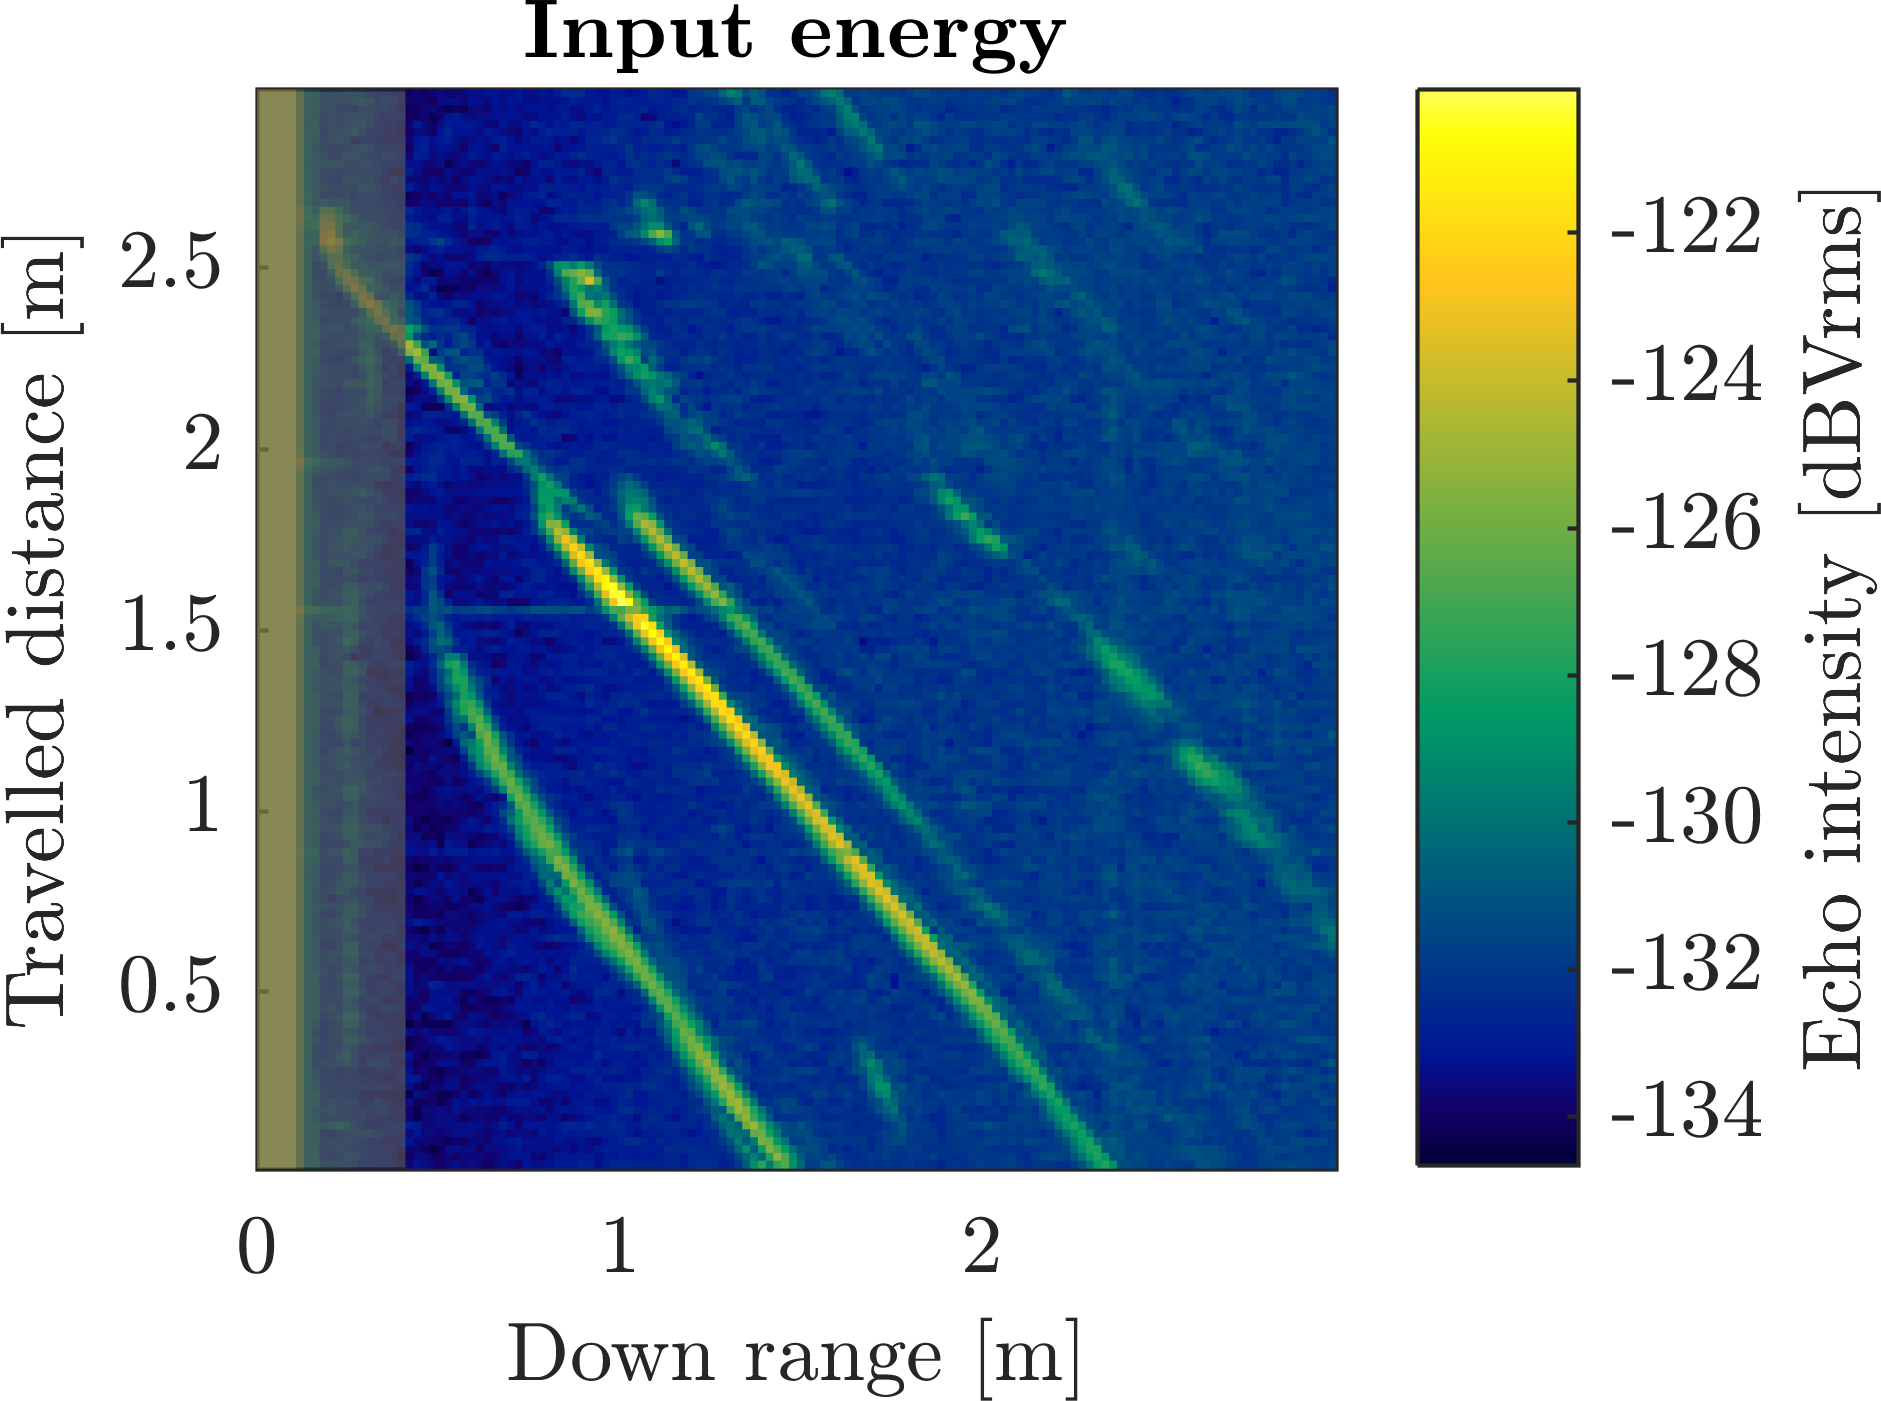
\includegraphics[width=\linewidth]{figures/fig_doa_sign_input.png}
        \caption{\label{fig:sauna_input}Echo intensity}
    \end{subfigure}%
    \hfill%
    \begin{subfigure}[b]{0.45\textwidth}
        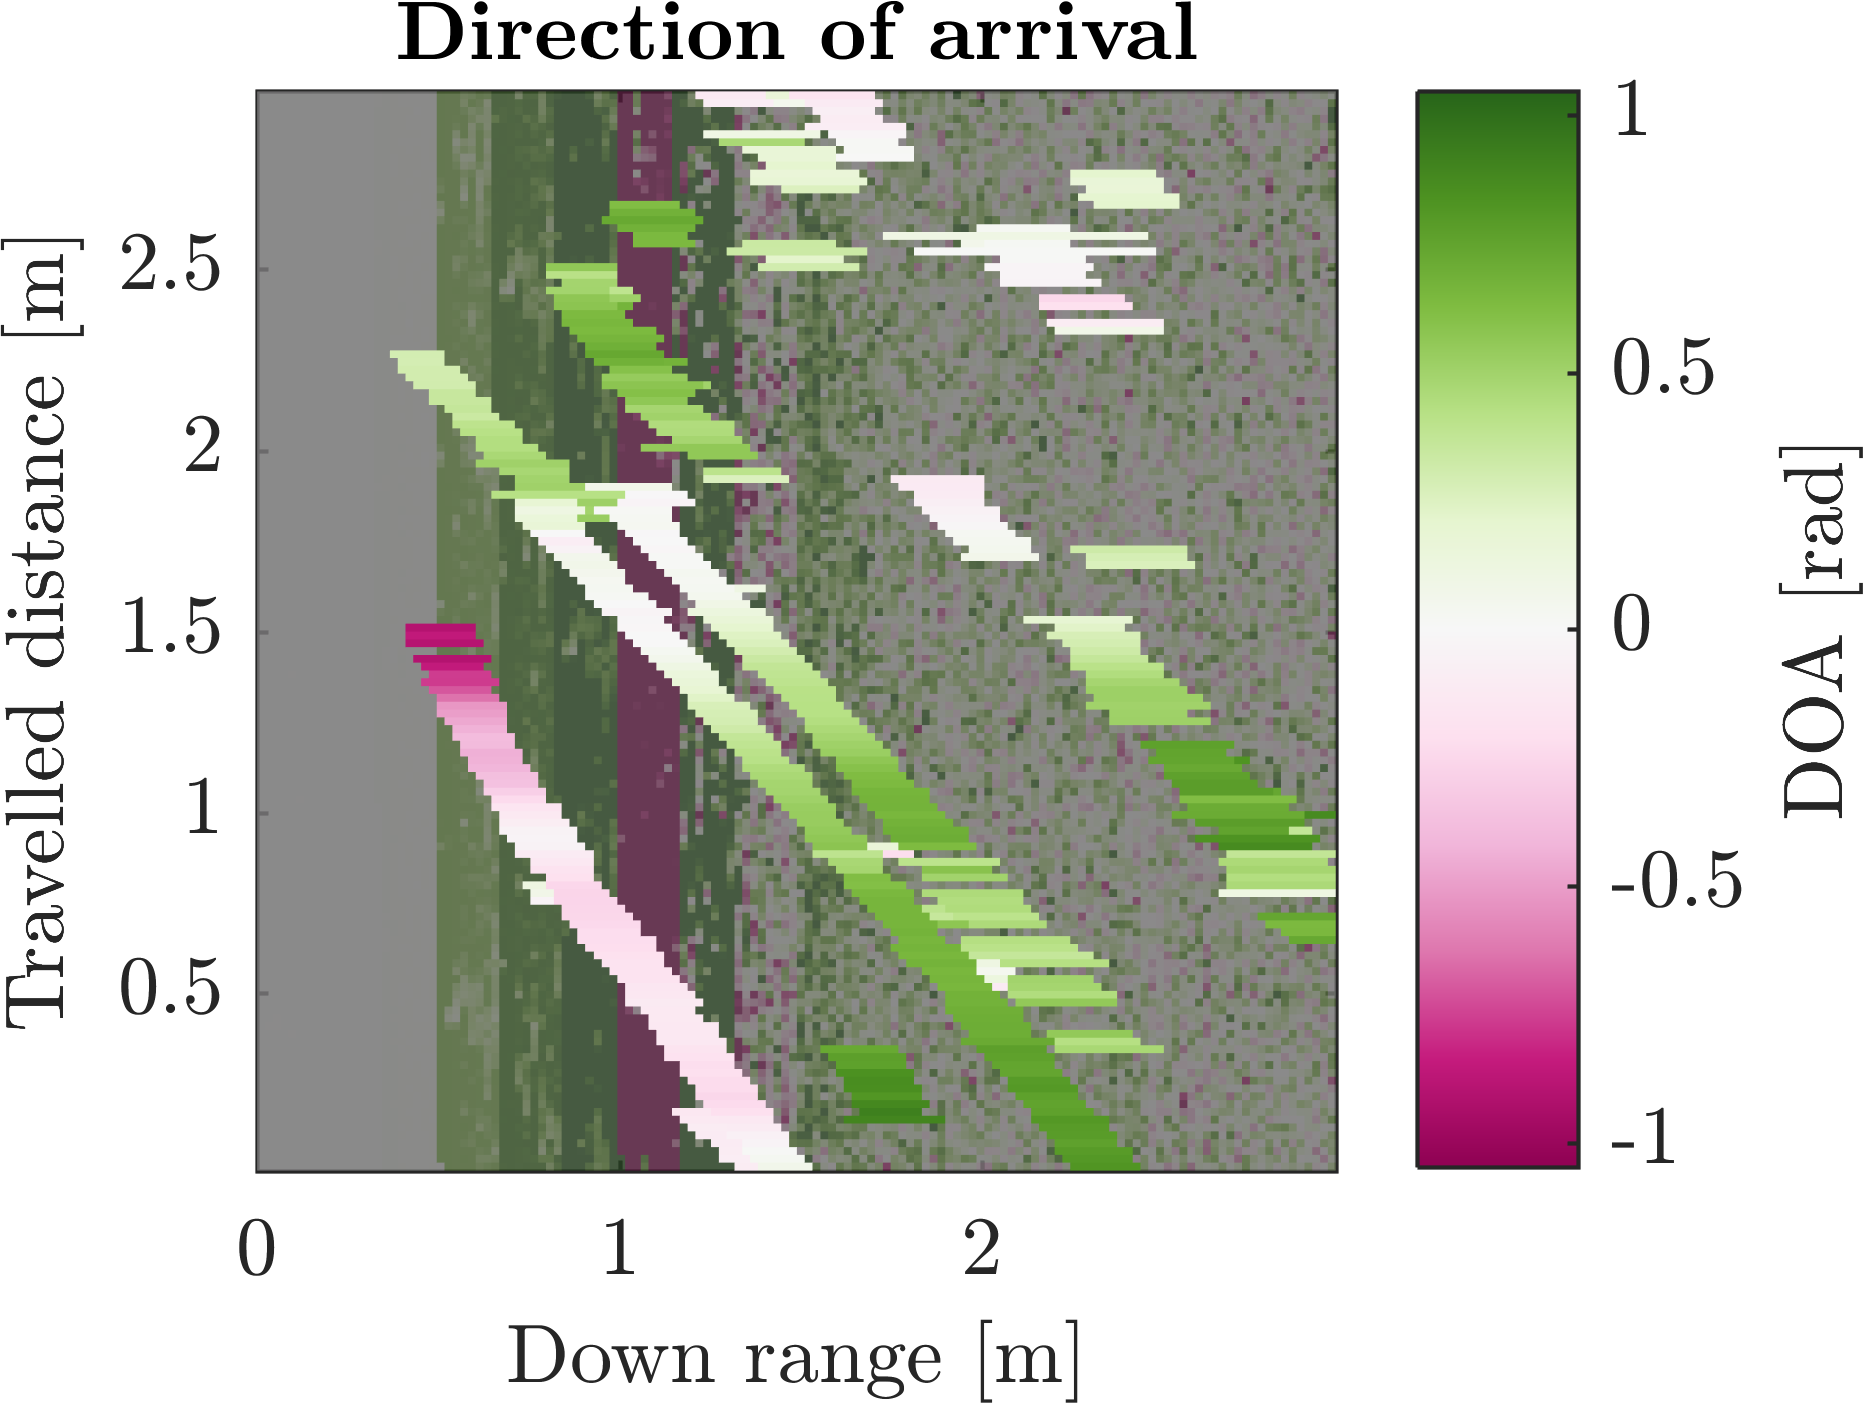
\includegraphics[width=\linewidth]{figures/fig_doa_sign_doa.png}
        \caption{\label{fig:sauna_doa}Direction of arrival estimation}
    \end{subfigure}
    \caption{Range profile and DOA of Sauna scan.}
    \label{fig:sauna}
\end{figure}

In fact, for the side-facing case, the smoothed DOA data also turned out
to be very good (angular error is usually less than \ang{10}). In combination with a sensor fusion approach, it might even be used to calculate a more precise
reprojection angle.

Both the forward- and side-facing geometry DOA data is sensitive to the rotation of the radar's antenna with respect to the radar motion path. When the DOA sign is used for angle ambiguity resolution, errors can thus appear at angles near \ang{0}. The effect does not have a drastic effect on map quality though, because angle sign errors do produce phantom targets at wrong map locations at large angles (e.g. \ang{90}), but still yield similar positions at small angles (i.e. mostly straight ahead).

\subsection{Multipath effects}\label{multipath-effects}

Multipath effects are a well-known problem in ground-based radar
applications \cite{Adams2012}. In situations where multi-path effects
are likely, there is a higher possibility that multiple versions of a
target's echo are visible, which can lead to detection of incorrect
angle and ranges. Luckily, in the recorded data almost no multipath
effects are obvious. The only scan that shows some effects is the
Torture Chamber. There, it seems like the radar waves bounce around a
bit in the area with highly reflective metal cabinets under the desk around (\SI{2}{m},\SI{2}{m}). The effect is that some targets are detected behind the wall behind the desk. It can be expected to be less noticeable in residential environments, which contain fewer (if any) metal corners.

\subsection{Object penetration}\label{object-penetration}

Some objects are penetrated by the radar waves. For example, in the
Attic and Basement scans, both the front and the back wall of a
plastic bottle can be seen. However, the plastic bottle was relatively
close to the sensor. On the other hand, in the scans with glass walls in
them (P,Q,R,S,U), no significant radar echo is picked up from the
(metal) chair legs behind the glass wall. This is because a typical
glass pane attenuates the \SI{60}{GHz} signal by about \SI{5.5}{dB} \cite{Lu2014}. In
effect, a radar sensor with higher transmission power might be able to
see through walls, but in the conducted experiments radar echos were to
faint to be picked up after the first bigger object (like a wall).
This is OK, because obstacles that are behind walls don't pose an immediate threat that needs to be circumnavigated. Through-wall visibility would mostly be interesting in slam applications that use the mapped objects for localization.

\subsection{Negative obstacles}\label{negative-obstacles}

\begin{figure}[htbp]
% 0.95 * 2832*2268/2124 / (2832*2268/2124 + 3024) = 0.475
% 0.95 * 3024 / (2832*2268/2124 + 3024) = 0.475
    \centering
    \begin{subfigure}[t]{.475\textwidth}
        \includegraphics[width=\textwidth]{gfx/pictures/cliff}
        \caption{For the negative obstacle detection tests the robot was driving on the cabinet.}
        \label{fig:cliff}
    \end{subfigure}%
    \hfill%
    \begin{subfigure}[t]{.475\textwidth}
        \includegraphics[width=\textwidth]{gfx/pictures/cliff_sensor}
        \caption{Sensor orientation for the Washroom scan: downward-facing vertical in an attempt to improve cliff detection}
        \label{fig:cliff_sensor}
    \end{subfigure}
\end{figure}

With scans V,W,X the negative obstacle detection capability was
analyzed in the environment shown in \cref{fig:cliff}. Cliffs, steps, and ditches are types of negative obstacles that cannot be traversed by the robot. In \cite{Jiang2015}, Jiang et al. claim that it is possible to detect this with UWB signals of various carrier frequencies. The experiments carried out for this thesis however did not show the same signal behaviour and it was not possible to reliably detect cliffs.

The Virtual Reality scan was carried out in the standard configuration
with a horizontal, slightly squinting, and not downwards angled sensor.
The assumption was that a part of the strong signal in the \SIrange{10}{20}{cm}
range was due to reflections from the floor, that should disappear when the
floor ends at a cliff. Visual inspection of the range profile however
shows only a extremely slight change in signal, e.g.~at cross range
\SIrange{0.8}{1.1}{m}, down range \SIrange{0.2}{0.25}{m}., where the floor could not reflect due to the radar sensor overhanging the cliff.

The Washroom scan has the sensor mounted in a vertical configuration and
downward facing (see \cref{fig:cliff_sensor}) instead to increase sensitivity to echo scattering from below. The echo intensity for cross range \SIrange{3.5}{4.5}{m} is indeed just
barely lower than \SIrange{0}{2}{m}, which matches up to where the sensor was over
the edge and over floor, respectively.

\begin{figure}[htbp]
    \centering
    \begin{subfigure}[t]{.475\textwidth}
        \includegraphics[max height=10cm,max width=10cm]{figures/fig_negobst}
        \caption{Regular plot.}
        \label{fig:negobst}
    \end{subfigure}%
    \hfill%
    \begin{subfigure}[t]{.475\textwidth}
        \includegraphics[max height=10cm,max width=10cm]{figures/fig_negobst_clipped}
        \caption{Zoomed and intensity-clipped for better visibility of the effect.}
        \label{fig:negobst_clipped}
    \end{subfigure}
    \caption{Input energy for the Washroom scan. Lower echo intensity at negative obstacles is hardly visible in the standard configuration.}
\end{figure}

TODO annotation-arrow pointing to darker region?

To limit the transmit crosstalk's blinding effect, the sensor was
mounted on a much higher position (on the RGBD camera mount) in the Xray
Room scan. One effect is that the robot chassis itself is constantly
visible at a distance of \SI{0.35}{cm} down range. At \SI{0.45}{cm} down range, the
floor echo is visible. There is one dip in intensity at \SI{2.5}{m} cross
range, where the sensor was not over floor. Overall the signal is
however not as conclusive as in the Washroom scan.

TODO annotation-arrow pointing to darker region?

\begin{figure}[htbp]
    \centering
    \begin{subfigure}[t]{.475\textwidth}
        \includegraphics[max height=10cm,max width=10cm]{figures/fig_negobst_xray}
        \caption{Regular plot.}
        \label{fig:negobst_xray}
    \end{subfigure}%
    \hfill%
    \begin{subfigure}[t]{.475\textwidth}
        \includegraphics[max height=10cm,max width=10cm]{figures/fig_negobst_xray_clipped}
        \caption{Zoomed and intensity-clipped for better visibility of the effect.}
        \label{fig:negobst_xray_clipped}
    \end{subfigure}
    \caption{Input energy for the XRay Room scan. Negative obstacles effect is not better with a higher-mounted vertical configuration.}
\end{figure}


Maybe the signal could be improved with improved background subtraction, but the three scans show that it is generally very hard to
detect negative obstacles with this sensor. A radar sensor of this type
will hence not be a viable replacement for regular cliff detection
sensors like the floor facing infrared distance sensors in the Kobuki
base.

\subsection{Cable detection}\label{cable-detection}

Cables on the floor are another interesting target that falls into the
category of obstacles being a very common occurrence in the real world,
but are hard to detect with conventional obstacle sensors. The Y (Is
There A Cable On The Floor) scan deals with the detection if this kind
of obstacle. For this, the same camera-mounted vertical configuration as
in X Ray Room was used. Again, there is a constant robot chassis echo at
down range \SI{0.35}{m}. As the robot is driving closer towards the power cable
on the floor, the cable's echo is visibly coming closer before it
disappears under the robot's chassis. The echos at \SI{0.9}{m} down range show
the two can towers at the end of the cable.

\begin{figure}[htp]
    \centering
    \includegraphics[max height=10cm,max width=10cm]{figures/fig_cable}
    \caption{Input energy of the Y (Is There A Cable On The Ground) scan. The center arc represents the echo of a cable on the floor as the robot approaches.}
    \label{fig:cable}
\end{figure}

Both the X Ray Room and Y (Is There A Cable On The Floor) introduce a
new geometry that lifts the radar sensor out of the two dimensional
mapping plane. The geometry is better described with the 3D case in \cref{geometry-for-the-3d-case}.

The results suggest that cables can be detected, but it might be hard to decide if the robot can safely drive over them.

\subsection{Minimum distance}\label{minimum-distance}

The constant noise from the transmission crosstalk leads to a high
minimum detection distance as explained in \cref{transmit-crosstalk-suppression}. The effect is that
targets can not be projected onto the map if the robot is too close to
them. This is an issue in the Sauna scan, where the glass wall right at
the beginning of the robot path cannot be mapped in its entirety.



%%%%%%%%%%%%%%%%%%%%%%%%%%%%%%%%%%%%%%%%%%%%%%%%%%%%%
\section{Comparison with other mapping techniques} \label{comparison-with-other-mapping-techniques}

While some of the radar reprojection maps speak for themselves, they
make more sense when compared to other mapping techniques. In the
following, SAR techniques, Laser slam, and RGBD slam are compared to the
radar reprojection.

\subsection{SAR}\label{sar-1}
Synthetic aperture radars make a lot of sense in applications
where the radar is moved over or through a map. The big difference to
this application is that ``professional'' SAR applications have radar
sensors that sit in vehicles that are not in the mapping plane.
Airplanes, satellites and even Submarines scan the earth like that.

There are a few examples for UWB radars being moved sideways (usually on a rail) in an effort to scan a scene with synthetic aperture radar.
Gregory L. Charvat's ``tin can'' radar \cite{Charvat2014} might be the most famous one, with many examples at \url{http://glcharvat.com/shortrange/}.
Another great resource was Henrik Forstén's Homemade Synthetic Aperture
Radar, documented in \cite{Forsten2015} (see \cref{fig:forsten}). He used an Omega-k algorithm \cite{Tolman2008} and Stolt interpolation \cite{Cumming2004} to correct the range migration arcs.

\begin{figure}
% 0.95 * 3264*817/2448 / (3264*817/2448 + 1299) = 0.43330076762
% 0.95 * 1299 / (3264*817/2448 + 1299) = 0.51669923238
    \begin{subfigure}[t]{0.43330076762\textwidth}
        \centering
        \includegraphics[max width=\linewidth]{gfx/pictures/forsten_1.jpg}
        \caption{Forstén's SAR setup. Source: \cite{Forsten2015}}
        \label{fig:forsten_1}
    \end{subfigure}%
    \hfill%
    \begin{subfigure}[t]{0.51669923238\textwidth}
        \centering
        \includegraphics[max width=\linewidth]{gfx/pictures/forsten_2.jpg}
        \caption{Forstén's SAR imagery agrees well with aerial imagery. Source: \cite{Forsten2015}}
        \label{fig:forsten_2}
    \end{subfigure}
    \caption{After omega-k processing and autofocusing, Forstén's synthetic aperture radar can create nice-looking broadside SAR imagery.}
    \label{fig:forsten}
\end{figure}


Forstén was able to greatly improve his data quality by use of a minimum-entropy based auto-focusing algorithm. The trick with this is that the radar needs to move in a very straight line, where the ``error in path linearity should be around less than tenth of a wavelength'' \cite{Forsten2015}. In Forstén's radar, this is about \SI{5}{mm}. However with the \SI{60}{GHz} Omniradar this is around \SI{0.5}{mm}. Keeping a straight line with less than half a millimeter of linearity error is not realistically achievable on the Kobuki platform.

One big inherent problem with synthetic aperture radar algorithms is
that basically all of them assume the radar to move in a straight line.
While changing the squint angle helps to deal with issues such as earth
curvature in satellite applications, SAR with curved or even arbitrary
paths is a challenging topic, particularly because auto-focusing, which
again relies on phase information, becomes more difficult
\cite{Axelsson2002}.

\subsection{RGBD}\label{rgbd-1}
The Kobuki robot was also carrying an Astra Orbbec Mini\footnote{\url{https://orbbec3d.com/astra-mini/}} strutured light depth camera. Using the Rtabmap \cite{Labbe2014} ROS package\footnote{\url{http://wiki.ros.org/rtabmap_ros}}, some 3D scans of the office environment where made. \cref{traditional-obstacle-sensors} already showed the shortcomings of lidar and RGBD sensors, but in this section the same \cref{fig:lidar_rgbd2,fig:rgbd_glasswall2} are compared with radar reprojection.

\Cref{fig:chairlegs} shows clearly that the radar reprojection contains horizontal chair legs, while the lidar scan does not. The scene in \cref{fig:rgbd_glasswall2} matches with the Underground scan, where the glass wall is clearly visible.

\begin{figure}
    \begin{subfigure}[t]{.485\textwidth}
        \centering
        \includegraphics[max width=\textwidth]{gfx/pictures/torturechamber_scene}
        \caption{View of the Torturechamber scan environment. Blue path is the robot's path.}
        \label{fig:chairs_scene}
    \end{subfigure}%
    \hfill%
    \begin{subfigure}[t]{.485\textwidth}
        \centering
        \includegraphics[max width=\textwidth]{gfx/results/torturechamber_map}
        \caption{Torturechamber reprojection map over lidar slam gridmap.}
        \label{fig:chairs_map}
    \end{subfigure}%
    \caption{In the Torturechamber scan, horizontal chair legs are visible in the reprojection map but not in the lidar scan.}
    \label{fig:chairlegs}
\end{figure}

\subsection{Lidar}\label{lidar-1}
As stated in \cref{kobuki}, the Kobuki robot used in the experiments was equipped with an RPLidar and a computing platform powerful enough to perform slam. Lidar slam is the standard approach when it comes to mapping the environment around a robot. After years of research and product development, even relatively cheap lidar systems like the RPLidar have acceptable range resolution. While they can't provide ground truth data (see problems with lidar data in \cref{traditional-obstacle-sensors}), it makes sense to compare the radar reprojection maps with laser scan maps. This is why all scans after Mancave have lidar maps associated.
%TODO?
Note that there is a bug in the rosbag to Matlab conversion that sometimes causes the complete map to be rotated against the lidar map by some degrees.

\chapter{Conclusion}\label{conclusion}

\section{Future Work}\label{future-work}

\subsection{Dynamic target rejection}\label{dynamic-target-rejection}

\subsection{Online mapping}\label{online-mapping}

The proof of concept implementation processes pre-recorded data. However
the algorithm is by no means limited to offline processing. Being very
much iterative and range scan line based it requires only the knowledge
of current and past, but not future scans. A live version of the
algorithm was not built, because the implementation was done in Matlab,
which does not run on arm processors natively. Matlab's Robotics Toolbox
does include a way to receive ROS messages live, but it is very slow and
would miss a lot of messages. This was tested by replaying a rosbag,
which works only at less than 10\% replay speed. This means that a 6
minute recording takes around 60 minutes to process. On the other hand,
just reading in all the messages in a rosbag takes around 3 minutes,
which is the reason the implementation was not done live. In a real
system (i.e.~not replayed from a rosbag) sending raw scan messages over
the network requires a lot of bandwidth, so the sampling frequency also
drops considerably.

An online system would probably have to be designed as a ROS node that
runs on the embedded platform.

Another topic that needs to be looked at for an online version is the
size of the reprojection map. It should automatically expand if a wider
area is necessary. This could be handled in a nice way with ROS's
\texttt{nav\_msgs/OccupancyGrid} messages and/or the
\href{http://wiki.ros.org/grid_map}{grid\_map package}. This would also
allow pretty and useful visualizations with RViz.

\subsection{ROS nodelet}\label{ros-nodelet}

The \texttt{omniradar\_node} ROS node spends quite some time on copying
the radar echo into the ros message that is to be sent out. As Austin
Hendrix points out in \textit{ROS answers}\footnote{\url{https://answers.ros.org/question/208801/how-to-have-no-copy-publishing-over-multiple-cores/?answer=208805\#post-id-208805}}, ``ROS doesn't provide intra-process, zero-copy publishing.
Nodelets can be run multi-threaded, so it is possible to have zero-copy
between different nodelets within a single nodelet manager''. Recording
a rosbag still involves copying the data, but in an online system a
nodelet-based reprojecting algorithm can be expected to bring a
reasonable performance improvement.

\subsection{Auto-thresholding}\label{auto-thresholding}

TODO

CFAR

\subsection{Realtime}\label{realtime}

An obstacle sensor's job is to provide information on impeding
collisions before it's too late. Thus it would be great to have the
system run under realtime constraints, so it can guarantee range
scanning and reprojection mapping to be finished within a known time
frame.

\subsection{Dynamic changing of sweep time and bandwidth}\label{dynamic-changing-of-sweep-time-and-bandwidth}

\subsection{Interference Investigation}\label{interference-investigation}

Since the 60 GHz band is ISM, other sources can be present, e.g.~the
IEEE 802.11ad standard \cite{IEEE2014} (``WiGig'') which enables very
high throughput wireless LAN operation in frequencies around 60GHz.
Commercial products using WiGig are already available and could cause
some interference with the 60GHz radar sensor. Detecting or avoiding
interference in the range signal would be an important topic if this
causes a lot of trouble.

\subsection{Ultrasound}\label{ultrasound}

Usually, ultrasound sensors measure the distance to the closest object.
However, K.C. Lee's project log of their ``Sonar for the visually
impaired'' project \cite{Lee2015} shows how cheap sensors can be hacked
to read a range profile that looks very similar (see figure \cref{fig:had_us}) to
what is used for the radar reprojection method. It might be possible to
adapt the algorithms in this thesis to use ultrasound sensors.

\begin{figure}[htp]
    \centering
    \includegraphics[max height=10cm,max width=10cm]{pictures/had_us}
    \caption{\label{fig:had_us}Range profile measurement with a hacked HCSR04 ultrasound module. Source: \cite{Lee2015}}
\end{figure}

Most ultrasound range sensors use the time of flight of a pulsed echo,
but FMCW-based ultrasound modules have been proposed
\cite{Battaglini2014} recently. With a range resolution of
\[dR = \frac{c_{sound, air}}{2 BW} = \frac{330 \frac{m}{s}}{2\cdot 12.5kHz} = 1.32 cm\]
the proposed sensor would be comparable to the Omniradar sensor's range
resolution and accuracy. However, for measurements to be very accurate
the speed of sound in air must be known as it depends on humidity and
temperature \cite{Bohn1987}.

For forward-facing geometry DOA is necessary to resolve the sign of the
reprojection angle. Sound waves do not not carry phase information, but
with a transducer array, direction of arrival can still be estimated
\cite{Kunin2010}.

Extension to ultrasound sensors would be a very interesting topic for
further work.

It might even be possible to use light waves with interferometric
modulated flash lidars and the right optics.

\subsection{3D case}\label{d-case}

Chapter \cref{idea} describes the geometry for 2D-cases. However, it
is possible to extend the concept to the three dimensional space if a
radar has more than two non-collinear receiving antennas, like
visualized in figure \cref{fig:2ddoa}. Horizontal DOA would be measured between
antennas at positions \(Rx1\) and \(Rx2\) while vertical DOA would be
measured between \(Rx1\) and \(Rx3\).

\begin{figure}[htp]
    \centering
    \def\svgwidth{5cm}
    \input{gfx/diagrams/outlook_doa.pdf_tex}
    \caption{\label{fig:2ddoa}Non-collinear triple receive antenna arrangement.}
\end{figure}

Reprojection mapping could then be used to build 3D occupancy maps. The
reprojection angle \(\alpha\) would then describe a circle at distance
\(R~cos(\alpha)\) around the radar path, on which the detected target
lies. Direction of arrival in horizontal and vertical planes would then
have to be used to pinpoint the target location on the circle.

\begin{figure}[htp]
    \centering
    \def\svgwidth{5cm}
    \input{gfx/diagrams/outlook_3d.pdf_tex}
    \caption{\label{fig:3dcase}A target detected at range \(R\) and relative Doppler speed corresponding to reprojection angle \(\alpha\) will be at a point on a circle (green) around the flight path (blue).}
\end{figure}

This holds also for the 2D-case: The possible locations for targets are
then at the intersection of reprojection cone circle and floor plane.

This would be useful on vehicles moving in 3D space, like the TUM RCS's
\href{https://www.rcs.ei.tum.de/forschung/mart/}{Modular Airborne
Real-Time Testbed (MART)} that was also used in other research and
publications \cite{Becker2015}.

\subsection{Single receive antennas on multiple sensors}\label{single-receive-antennas-on-multiple-sensors}

Direction of arrival is a good solution to resolve the ambiguities
presented in the general 2D-case \cref{geometry-for-the-general-case} and 3D-case geometry (\cref{fig:3dcase}) for a
sensor with a sufficient number of antennas. However, it should also be
possible to use multiple, spatially separated sensors instead. Each
sensor measures a reprojection angle. A target visible to both sensors
can then be localized unambiguously with triangulation.

TODO

3D scenario. standard case: two intersecting spheres --\textgreater{}
intersection circle doppler reprojection case: angle --\textgreater{}
cones with intersecting base edge -\textgreater{} two interesection
points (DOA to resolve, or high flying drone to assume)

\section{Conclusion}\label{conclusion-1}

Mobile robots still struggle to detect some obstacles that are invisible
to their conventional sensors. Radar sensors have a big potential to
improve obstacle avoidance. With reprojection mapping, this thesis
proposes a novel method to create an obstacle map without having to
steer the radar beam.

A proof-of-concept implementation of the reprojection mapping produced
obstacle maps from the radar scans of the experiments for this thesis.
The maps prove that some previously undetectable obstacles, like glass
walls and office chair legs, can now be detected and mapped.

The next step on the way to a mobile indoor robot proficiently
navigating real-world environments should be the implementation of an
online version of reprojection mapping. This will also show if the
results need to be further improved with more advanced noise rejection.

TODO



% Anhang
\clearpage
\begin{appendix}

\chapter{List of Scans}

{

\rowcolors{1}{ColorAlternatedRow}{}

\begin{tabularx}{\textwidth}{%
  >{\setlength{\hsize}{.31\hsize}\raggedright\arraybackslash}X%
  >{\setlength{\hsize}{.13\hsize}\raggedright\arraybackslash}X%
  >{\setlength{\hsize}{.13\hsize}\raggedright\arraybackslash}X%
  >{\setlength{\hsize}{.13\hsize}\raggedright\arraybackslash}X%
  >{\setlength{\hsize}{.10\hsize}\centering\arraybackslash}X%
  >{\setlength{\hsize}{.10\hsize}\centering\arraybackslash}X%
  >{\setlength{\hsize}{.10\hsize}\centering\arraybackslash}X%
}%

\hiderowcolors
%
%\caption{Scan parameters}
%
\toprule
    Name & Sweep & Orient. & Squint & Horn   & Map    & TF     \\
\midrule
\endhead
%
\midrule
\multicolumn{6}{r}{Continued on next page} \\
\endfoot
%
\bottomrule
\endlastfoot
\showrowcolors
%
Attic                             & 5ms        & H           & 90°    & \cmark & \xmark & \xmark \\
Basement                          & 5ms        & H           & 90°    & \cmark & \xmark & \xmark \\
Cafeteria                         & 5ms        & H           & 90°    & \cmark & \xmark & \xmark \\
Dungeon                           & 5ms        & V           & 20°    & \cmark & \xmark & \xmark \\
Entryway                          & 5ms        & V           & 20°    & \cmark & \xmark & \xmark \\
Fallout shelter                   & 5ms        & V           & 20°    & \cmark & \xmark & \xmark \\
Garden                            & 5ms        & V           & 20°    & \cmark & \xmark & \xmark \\
Home cinema                       & 5ms        & V           & 20°    & \cmark & \xmark & \xmark \\
Indoor swimming pool              & 5ms        & V           & 20°    & \cmark & \xmark & \xmark \\
Jail cell                         & 5ms        & H           & 20°    & \cmark & \xmark & \xmark \\
Kitchen                           & 5ms        & H           & 20°    & \xmark & \xmark & \xmark \\
Lobby                             & 5ms        & H/I         & 0°     & \xmark & \xmark & \xmark \\
Mancave                           & 5ms        & H/I         & 0°     & \xmark & \xmark & \xmark \\
Nirvana                           & 5ms        & H/I         & 0°     & \xmark & \cmark & \xmark \\
Orbit                             & 5ms        & H/I         & 0°     & \xmark & \cmark & \xmark \\
Public Restroom                   & 5ms        & H/I         & 0°     & \xmark & \cmark & \cmark \\
Queue                             & 20ms       & H/I         & 0°     & \xmark & \cmark & \cmark \\
Racetrack                         & 2ms        & H/I         & 0°     & \xmark & \cmark & \cmark \\
Sauna                             & 2.5ms      & H/I         & 0°     & \xmark & \cmark & \cmark \\
Torture Chamber                   & 2.5ms      & H/I         & 45°    & \xmark & \cmark & \cmark \\
Underground                       & 2.5ms      & H/I         & 45°    & \xmark & \cmark & \cmark \\
Virtual Reality                   & 2.5ms      & H/I         & 45°    & \xmark & \cmark & \cmark \\
Washroom                          & 2.5ms      & V           & 45°    & \xmark & \cmark & \cmark \\
Xray-Room                         & 2.5ms      & V           & 0°     & \xmark & \cmark & \cmark \\
Y is there a cable on the floor   & 5ms        & V           & 0°     & \xmark & \cmark & \cmark \\
Z                                 &            &             &        &        &        &        \\

\bottomrule
\end{tabularx}
}



% Attic & \raisebox{-.5\height}{\includegraphics[width=4cm]{gfx/results/attic_input}} & \raisebox{-.5\height}{\includegraphics[width=4cm]{gfx/results/attic_doppler}} & \raisebox{-.5\height}{\includegraphics[width=4cm]{gfx/results/attic_doa}} & \raisebox{-.5\height}{\includegraphics[width=4cm]{gfx/results/attic_reprojection}} & 5ms & H & 90° & \cmark & \xmark & \xmark \\
% Basement & \raisebox{-.5\height}{\includegraphics[width=4cm]{gfx/results/basement_input}} & \raisebox{-.5\height}{\includegraphics[width=4cm]{gfx/results/basement_doppler}} & \raisebox{-.5\height}{\includegraphics[width=4cm]{gfx/results/basement_doa}} & \raisebox{-.5\height}{\includegraphics[width=4cm]{gfx/results/basement_reprojection}} & 5ms & H & 90° & \cmark & \xmark & \xmark \\
% Cafeteria                         & \raisebox{-.5\height}{\includegraphics{gfx/results/cafeteria_input}}          & \raisebox{-.5\height}{\includegraphics{gfx/results/cafeteria_doppler}}          & \raisebox{-.5\height}{\includegraphics{gfx/results/cafeteria_doa}}          & \raisebox{-.5\height}{\includegraphics{gfx/results/cafeteria_reprojection}}          & 5ms        & H           & 90°    & \cmark & \xmark & \xmark \\
% Dungeon                           & \raisebox{-.5\height}{\includegraphics{gfx/results/dungeon_input}}            & \raisebox{-.5\height}{\includegraphics{gfx/results/dungeon_doppler}}            & \raisebox{-.5\height}{\includegraphics{gfx/results/dungeon_doa}}            & \raisebox{-.5\height}{\includegraphics{gfx/results/dungeon_reprojection}}            & 5ms        & V           & 20°    & \cmark & \xmark & \xmark \\
% Entryway                          & \raisebox{-.5\height}{\includegraphics{gfx/results/entryway_input}}           & \raisebox{-.5\height}{\includegraphics{gfx/results/entryway_doppler}}           & \raisebox{-.5\height}{\includegraphics{gfx/results/entryway_doa}}           & \raisebox{-.5\height}{\includegraphics{gfx/results/entryway_reprojection}}           & 5ms        & V           & 20°    & \cmark & \xmark & \xmark \\
% Fallout shelter                   & \raisebox{-.5\height}{\includegraphics{gfx/results/falloutshelter_input}}     & \raisebox{-.5\height}{\includegraphics{gfx/results/falloutshelter_doppler}}     & \raisebox{-.5\height}{\includegraphics{gfx/results/falloutshelter_doa}}     & \raisebox{-.5\height}{\includegraphics{gfx/results/falloutshelter_reprojection}}     & 5ms        & V           & 20°    & \cmark & \xmark & \xmark \\
% Garden                            & \raisebox{-.5\height}{\includegraphics{gfx/results/garden_input}}             & \raisebox{-.5\height}{\includegraphics{gfx/results/garden_doppler}}             & \raisebox{-.5\height}{\includegraphics{gfx/results/garden_doa}}             & \raisebox{-.5\height}{\includegraphics{gfx/results/garden_reprojection}}             & 5ms        & V           & 20°    & \cmark & \xmark & \xmark \\
% Home cinema                       & \raisebox{-.5\height}{\includegraphics{gfx/results/homecinema_input}}         & \raisebox{-.5\height}{\includegraphics{gfx/results/homecinema_doppler}}         & \raisebox{-.5\height}{\includegraphics{gfx/results/homecinema_doa}}         & \raisebox{-.5\height}{\includegraphics{gfx/results/homecinema_reprojection}}         & 5ms        & V           & 20°    & \cmark & \xmark & \xmark \\
% Indoor swimming pool              & \raisebox{-.5\height}{\includegraphics{gfx/results/indoorswimmingpool_input}} & \raisebox{-.5\height}{\includegraphics{gfx/results/indoorswimmingpool_doppler}} & \raisebox{-.5\height}{\includegraphics{gfx/results/indoorswimmingpool_doa}} & \raisebox{-.5\height}{\includegraphics{gfx/results/indoorswimmingpool_reprojection}} & 5ms        & V           & 20°    & \cmark & \xmark & \xmark \\
% Jail cell                         & \raisebox{-.5\height}{\includegraphics{gfx/results/jailcell_input}}           & \raisebox{-.5\height}{\includegraphics{gfx/results/jailcell_doppler}}           & \raisebox{-.5\height}{\includegraphics{gfx/results/jailcell_doa}}           & \raisebox{-.5\height}{\includegraphics{gfx/results/jailcell_reprojection}}           & 5ms        & H           & 20°    & \cmark & \xmark & \xmark \\
% Kitchen                           & \raisebox{-.5\height}{\includegraphics{gfx/results/kitchen_input}}            & \raisebox{-.5\height}{\includegraphics{gfx/results/kitchen_doppler}}            & \raisebox{-.5\height}{\includegraphics{gfx/results/kitchen_doa}}            & \raisebox{-.5\height}{\includegraphics{gfx/results/kitchen_reprojection}}            & 5ms        & H           & 20°    & \xmark & \xmark & \xmark \\
% Lobby                             & \raisebox{-.5\height}{\includegraphics{gfx/results/lobby_input}}              & \raisebox{-.5\height}{\includegraphics{gfx/results/lobby_doppler}}              & \raisebox{-.5\height}{\includegraphics{gfx/results/lobby_doa}}              & \raisebox{-.5\height}{\includegraphics{gfx/results/lobby_reprojection}}              & 5ms        & H/I         & 0°     & \xmark & \xmark & \xmark \\
% Mancave                           & \raisebox{-.5\height}{\includegraphics{gfx/results/mancave_input}}            & \raisebox{-.5\height}{\includegraphics{gfx/results/mancave_doppler}}            & \raisebox{-.5\height}{\includegraphics{gfx/results/mancave_doa}}            & \raisebox{-.5\height}{\includegraphics{gfx/results/mancave_reprojection}}            & 5ms        & H/I         & 0°     & \xmark & \xmark & \xmark \\
% Nirvana                           & \raisebox{-.5\height}{\includegraphics{gfx/results/nirvana_input}}            & \raisebox{-.5\height}{\includegraphics{gfx/results/nirvana_doppler}}            & \raisebox{-.5\height}{\includegraphics{gfx/results/nirvana_doa}}            & \raisebox{-.5\height}{\includegraphics{gfx/results/nirvana_reprojection}}            & 5ms        & H/I         & 0°     & \xmark & \cmark & \xmark \\
% Orbit                             & \raisebox{-.5\height}{\includegraphics{gfx/results/orbit_input}}              & \raisebox{-.5\height}{\includegraphics{gfx/results/orbit_doppler}}              & \raisebox{-.5\height}{\includegraphics{gfx/results/orbit_doa}}              & \raisebox{-.5\height}{\includegraphics{gfx/results/orbit_reprojection}}              & 5ms        & H/I         & 0°     & \xmark & \cmark & \xmark \\
% Public Restroom                   & \raisebox{-.5\height}{\includegraphics{gfx/results/publicrestroom_input}}     & \raisebox{-.5\height}{\includegraphics{gfx/results/publicrestroom_doppler}}     & \raisebox{-.5\height}{\includegraphics{gfx/results/publicrestroom_doa}}     & \raisebox{-.5\height}{\includegraphics{gfx/results/publicrestroom_reprojection}}     & 5ms        & H/I         & 0°     & \xmark & \cmark & \cmark \\
% Queue                             & \raisebox{-.5\height}{\includegraphics{gfx/results/queue_input}}              & \raisebox{-.5\height}{\includegraphics{gfx/results/queue_doppler}}              & \raisebox{-.5\height}{\includegraphics{gfx/results/queue_doa}}              & \raisebox{-.5\height}{\includegraphics{gfx/results/queue_reprojection}}              & 20ms       & H/I         & 0°     & \xmark & \cmark & \cmark \\
% Racetrack                         & \raisebox{-.5\height}{\includegraphics{gfx/results/racetrack_input}}          & \raisebox{-.5\height}{\includegraphics{gfx/results/racetrack_doppler}}          & \raisebox{-.5\height}{\includegraphics{gfx/results/racetrack_doa}}          & \raisebox{-.5\height}{\includegraphics{gfx/results/racetrack_reprojection}}          & 2ms        & H/I         & 0°     & \xmark & \cmark & \cmark \\
% Sauna                             & \raisebox{-.5\height}{\includegraphics{gfx/results/sauna_input}}              & \raisebox{-.5\height}{\includegraphics{gfx/results/sauna_doppler}}              & \raisebox{-.5\height}{\includegraphics{gfx/results/sauna_doa}}              & \raisebox{-.5\height}{\includegraphics{gfx/results/sauna_reprojection}}              & 2.5ms      & H/I         & 0°     & \xmark & \cmark & \cmark \\
% Torture Chamber                   & \raisebox{-.5\height}{\includegraphics{gfx/results/torturechamber_input}}     & \raisebox{-.5\height}{\includegraphics{gfx/results/torturechamber_doppler}}     & \raisebox{-.5\height}{\includegraphics{gfx/results/torturechamber_doa}}     & \raisebox{-.5\height}{\includegraphics{gfx/results/torturechamber_reprojection}}     & 2.5ms      & H/I         & 45°    & \xmark & \cmark & \cmark \\
% Underground                       & \raisebox{-.5\height}{\includegraphics{gfx/results/underground_input}}        & \raisebox{-.5\height}{\includegraphics{gfx/results/underground_doppler}}        & \raisebox{-.5\height}{\includegraphics{gfx/results/underground_doa}}        & \raisebox{-.5\height}{\includegraphics{gfx/results/underground_reprojection}}        & 2.5ms      & H/I         & 45°    & \xmark & \cmark & \cmark \\




\begin{figure}
    % \centering
    \begin{subfigure}[b]{0.25\textwidth}
        \centering
        \includegraphics[width=.9\textwidth]{gfx/results/attic_input.png}
        \caption{\small Input energy}
    \end{subfigure}%
    \begin{subfigure}[b]{0.25\textwidth}  
        \centering 
        \includegraphics[width=.9\textwidth]{gfx/results/attic_doppler.png}
        \caption{\small Doppler estimation}
    \end{subfigure}%
    \begin{subfigure}[b]{0.25\textwidth}   
        \centering 
        \includegraphics[width=.9\textwidth]{gfx/results/attic_doa.png}
        \caption{\small Direction of Arrival}
    \end{subfigure}%
    \begin{subfigure}[b]{0.25\textwidth}   
        \centering 
        \includegraphics[width=.9\textwidth]{gfx/results/attic_reprojection.png}
        \caption{\small Reprojection Map}
    \end{subfigure}%
    \caption{Attic scan}
\end{figure}

\begin{figure}
    % \centering
    \begin{subfigure}[b]{0.25\textwidth}
        \centering
        \includegraphics[width=.9\textwidth]{gfx/results/basement_input.png}
        \caption{\small Input energy}
    \end{subfigure}%
    \begin{subfigure}[b]{0.25\textwidth}  
        \centering 
        \includegraphics[width=.9\textwidth]{gfx/results/basement_doppler.png}
        \caption{\small Doppler estimation}
    \end{subfigure}%
    \begin{subfigure}[b]{0.25\textwidth}   
        \centering 
        \includegraphics[width=.9\textwidth]{gfx/results/basement_doa.png}
        \caption{\small Direction of Arrival}
    \end{subfigure}%
    \begin{subfigure}[b]{0.25\textwidth}   
        \centering 
        \includegraphics[width=.9\textwidth]{gfx/results/basement_reprojection.png}
        \caption{\small Reprojection Map}
    \end{subfigure}%
    \caption{Basement scan}
\end{figure}

TODO



\end{appendix}

\listoffigures
\listoftables

% Index
\clearpage
\printindex

% Literaturverzeichnis
%\nocite{wasauchimmer}
\clearpage
%\bibliographystyle{geralpha}
\bibliographystyle{gerplain}
\bibliography{mendeley}

\end{document}
